% Academic revision prepared from songlines_unified(2).tex.
% Revision goals: conventional problem-method-results-scope structure;
% cautious claim language; terminology consistency; preservation of all
% equations, tables, labels, references, and reported numerical results.
\documentclass{article}

\usepackage{neurips_2026}

\usepackage[utf8]{inputenc}
\usepackage[T1]{fontenc}
\usepackage{hyperref}
\hypersetup{hidelinks}
\usepackage{url}
\usepackage{booktabs}
\usepackage{amsfonts}
\usepackage{amssymb}
\usepackage{amsmath}
\usepackage{nicefrac}
\usepackage{microtype}
\usepackage{xcolor}
\usepackage{graphicx}
\graphicspath{{./}}
\usepackage{array}
\usepackage{enumitem}
\usepackage{placeins}
\usepackage{tikz}
\usetikzlibrary{arrows.meta,positioning}

\newcommand{\method}[1]{\texttt{#1}}
\newcommand{\wstar}{W^{\star}}
\newcommand{\rwstar}{RW^{\star}}
\newcommand{\mstar}{M^{\star}}
\newcommand{\cstar}{C^{\star}}
\newcommand{\phiroute}{\varphi_{\mathrm{route}}}

\setcounter{tocdepth}{2}

\title{Q/R/M/C: Stage-Decomposed Evaluation of Memory-Grounded Agents}

\begin{document}
\maketitle
\begin{abstract}
End-to-end success rates do not identify which component of a
memory-based navigation pipeline is responsible for failure. We
introduce Q/R/M/C, an operational evaluation protocol that separates
query formation, retrieval satisfaction, target materialization, and
completion after retrieval. The four stage events are defined at the
log level and their conditional rates factorize semantic-path
completion for systems that expose an explicit query and target-lock
interface. The contribution is therefore methodological rather than a
new probabilistic theorem: the factorization follows the chain rule,
whereas the value of the framework lies in making intermediate
failure locations observable and comparable. We evaluate the protocol
on symbolic single-agent tasks, four multi-agent memory
architectures, learned communication policies, local LLM agents, and
three third-party agent stacks. In the single-agent benchmark, oracle
interventions distinguish retrieval-limited hazard recovery from
downstream-limited goal-region rejoin. Log analysis further shows that
the apparent retrieval failure is a candidate-availability
problem: eligible candidates are absent at $91\%$ of decision points,
while ranking precision is $96.9\%$ when candidates are present. A
stage-wise oracle ladder then separates the causes per task: on
hazard recovery the absences are phrase-graph grounding failures
whose repair removes the symptom but not the failure --- the binding
constraint is the semantic quality of the designated candidates ---
whereas on goal-region rejoin they are genuine coverage-driven
retrieval emptiness. In
the multi-agent benchmark, communication cadence changes the location
of the bottleneck. Faster exchange improves materialization but
reduces completion under scarce targets because agents commit to the
same resources; the corresponding stage-rate slopes are moderate and
cluster-robust, and mean time to success has a shallow interior
minimum at $K=8$ when conditioned on successful episodes. The same
logging contract localizes engineered failures in LLM and third-party
agent stacks, while also revealing when Q/R/M/C is not separately
observable in opaque learned policies. Q/R/M/C should therefore be
interpreted as a diagnostic layer for systems with an explicit memory
interface, not as a replacement for end-to-end evaluation, policy
probing, or causal mediation analysis. The primary evidence is based
on controlled grid-world experiments, with directional checks on
BabyAI, VMAS, TextNav, and external agent frameworks.
\par\medskip\noindent\textbf{We claim.} End-to-end success is
insufficient for diagnosing memory-grounded agent behavior. For systems
that expose an explicit query and target-commitment interface, the
Q/R/M/C contract separates query formation, retrieval satisfaction,
target materialization, and post-retrieval completion into observable
and estimable stages, thereby localizing failure mechanisms and
bottleneck shifts that aggregate task metrics conflate.
\end{abstract}

\FloatBarrier
\section{Introduction}

\begin{figure}[t]
  \centering
  
\includegraphics[width=\linewidth]{figures/fig_hero_qrmc.pdf}
  \caption{Q/R/M/C decomposes one semantic-navigation episode into four
  observable stages. \textbf{Top:} the four stages and their event-level
  definitions. \textbf{(a)} A successful water-search episode anchors at
  one event per stage, producing logged starred events
  $Q^\star, R^\star, M^\star, C^\star$. \textbf{(b)} The same scalar
  ``end-to-end success'' summary masks qualitatively different failures
  on the four single-agent task families: water and rest are strong;
  goal-region rejoin (FourRooms) is downstream-limited; hazard recovery
  (LavaGapS7) is retrieval-limited (oracle interventions, \S\ref{p1:sec:oracle}).}
  \label{p1:fig:hero}
\end{figure}

Memory-based navigation is commonly evaluated through a final success
indicator or an aggregate return. These measures are necessary, but
they do not distinguish failures caused by an absent query, an empty
or incorrect retrieval, an inability to convert retrieved evidence
into an actionable target, or a failure of the controller after a
valid target has been selected. This distinction is particularly
important when the target is specified semantically rather than by a
fixed coordinate. In such tasks, the agent must first represent the
intent, retrieve a place that satisfies it, commit to a concrete
referent, and execute a trajectory to that referent.

We propose Q/R/M/C as a stage-decomposed evaluation protocol for this
setting. The protocol records four events: query formation ($Q$),
retrieval satisfaction ($R$), target materialization ($M$), and
completion after materialization ($C$). The nested episode-level
events factorize semantic-path completion, whereas the operational
per-query and per-tick rates provide a practical diagnostic view of
the same pipeline. The factorization is intentionally elementary. Its
purpose is to specify a logging contract under which intermediate
failure locations can be estimated consistently from trajectory
records.

The empirical analysis addresses three questions. First, does the
stage decomposition distinguish task families that have similar final
success but fail for different reasons? Second, how does the location
of the bottleneck change when memory becomes a shared resource among
multiple agents? Third, does the same event contract remain useful on
learned and language-agent systems whose internal representations
differ from the symbolic reference implementation?

The single-agent experiments show that stage localization changes the
interpretation of the benchmark. Hazard recovery is retrieval-limited:
replacing retrieval or materialization with an oracle produces a
substantial success increase, whereas replacing the controller does
not. Goal-region rejoin is instead limited downstream of retrieval.
Within the retrieval-limited task, the detailed logs further identify
candidate generation as the principal failure: the memory returns no
eligible record at most decision points, despite near-perfect ranking
when a record exists --- and a stage-wise oracle ladder splits these
absences into phrase-graph grounding failures and true coverage
emptiness (\S\ref{p1:sec:refined-attribution}). The multi-agent analysis shows a different
phenomenon. As broadcast cadence increases, fresher peer memory
improves materialization, but the same information synchronizes
commitments and reduces completion under target scarcity. The result
is a measurable migration of the bottleneck between the $M$ and $C$
stages.

The contributions of this paper are as follows:
\begin{enumerate}[leftmargin=20pt,itemsep=2pt,topsep=2pt]
\item We define log-level operational and nested Q/R/M/C events for
single- and multi-agent memory-based navigation and state the
conditions under which their conditional rates are estimable.
\item We validate the protocol through stage-specific oracle
interventions and dissect a candidate-availability limitation that is
invisible to end-to-end success: a stage-wise oracle ladder splits it
into phrase-graph grounding failures (whose repair does not restore
success) and coverage-driven retrieval emptiness, excluding ranking,
thresholding, and perception as causes.
\item We characterize a cadence-dependent materialization--completion
trade-off in a large multi-agent sweep and relate it to foreign
evidence and target occupancy.
\item We evaluate the same event contract on learned communication
policies, local LLM agents, and three third-party agent frameworks,
thereby separating structural task failures from model- and
framework-specific behavior.
\end{enumerate}

The framework has a clear boundary. Separate Q/R/M/C rates require an
observable query and commitment interface. For opaque policies, the
protocol can identify the absence of stage observability but cannot
recover latent stages that the architecture does not expose. In
addition, the four-rate product describes completion through the
semantic retrieval path rather than all possible routes to task
success. These restrictions are treated as part of the measurement
contract rather than hidden assumptions.

The remainder of the paper defines the event semantics and estimators,
reports the single- and multi-agent studies, evaluates portability to
language-agent and third-party stacks, and discusses limitations and
reproducibility.

\section{The Q/R/M/C decomposition}
\label{p1:sec:framework}

\subsection{Problem formulation and notation}
\label{p1:sec:notation}

The agent operates in a partially observable navigation environment.
At each step it receives an observation $o_t$, maintains a memory
state $\mathcal{M}_t$, and forms a query $q_t$ encoding the current
task intent. A retrieval step returns a candidate set of places
matching $q_t$ from $\mathcal{M}_t$; a chosen candidate is
materialized into an actionable target; a local controller executes
actions until either the target is reached or the episode times out.
The target is not a coordinate but a semantic pattern, so success is a
function of the chosen candidate's semantic profile, not of any
pre-supplied coordinate.

Habitat, AI2-THOR, and ProcTHOR made visually rich navigation
evaluation standard
\citep{savva2019habitat,kolve2017ai2thor,deitke2022procthor}. We
deliberately focus on MiniGrid-class environments to obtain clean and
reproducible stage measurements, and use BabyAI only as a portability
check. We do not claim to solve LLM-agent memory here; rather, we
argue that the same Q/R/M/C decomposition is a useful template for
evaluating memory-grounded agent decisions beyond navigation.

The central empirical question is therefore not just whether the agent
succeeds, but \emph{which stage fails first} when it does not. Two
related measurement layers are used, with distinct notation.
\textbf{Operational events} (lowercase) are counted per query attempt:
$q_t$ --- a valid query object was emitted; $r^{\mathrm{set}}_t$ ---
the returned candidate set is non-empty, i.e.\ at least one stored
record satisfies the query predicate on the \emph{agent's} side;
$r_t$ --- a retrieved candidate is correct on the \emph{evaluator's}
side, under the evaluation correspondence $\Gamma$ between memory
records and world entities (\S\ref{p1:sec:event-semantics});
$m_t$ --- a candidate was materialized into an actionable target.
Separating $r^{\mathrm{set}}$ from $r$ keeps two different retrieval
failures apart: an empty candidate set (nothing satisfies the
predicate) and an incorrect candidate set (something satisfies the
predicate but does not correspond to a true target).
\emph{Completion after retrieval} is an episode-level indicator.
\textbf{Nested episode-level events} (starred)
$Q^\star \Rightarrow R^\star \Rightarrow M^\star \Rightarrow C^\star$
are used in the factorization below and audited in
\S\ref{p1:sec:validation}. Full operational definitions are given in
Appendix~\ref{p1:app:estimators}.

\textbf{Notation.} The four stages are $Q$, $R$, $M$, $C$ with episode-level starred events $Q^\star,R^\star,M^\star,C^\star\!\in\!\{0,1\}$, nested by construction. $P(\cdot)$ denotes the population probability; $\hat{P}(\cdot)$ its empirical-frequency estimator. \textbf{The letter $M$ always refers to the Materialization stage; the number of targets in the multi-agent environment is written $T$ (not $M$, constraint $T{\le}N$, ``scarcity'' = $N{>}T$).} Other symbols: $\mathcal{C}_K$ peer-broadcast protocol with cadence $K$, $\mathcal{M}_{-i}^{(K)}$ peer memory snapshots, $\mathcal{O}_{-i}$ peer occupancy, $\nu(\cdot)$ freshness functional, $\Phi(K){=}P(M^\star|R^\star;K)\!\cdot\!P(C^\star|M^\star;K)$, $t_{\mathrm{succ}}$ mean time-to-success. Full symbol table in Appendix~\ref{p1:app:notation}.

\subsection{Single-agent factorization}
\label{p1:sec:single-theory}

Let $Y$ denote overall episode success, and let
$Q^\star, R^\star, M^\star, C^\star$ denote the nested episode-level
semantic-path events. The framework factorizes \emph{semantic-path
completion} rather than raw task success:
\[
Q^\star \rightarrow R^\star \rightarrow M^\star \rightarrow C^\star.
\]
We deliberately separate three claims of different strength: an
algebraic identity that holds by construction, a statistical statement
about estimation, and a structural assumption that is needed only for
a mechanism-level reading.

\paragraph{Proposition 1 (algebraic decomposition; no assumptions).}
Because the starred events are nested
($C^\star \subseteq M^\star \subseteq R^\star \subseteq Q^\star$), the
chain rule gives, identically,
\[
P(C^\star)
=
P(Q^\star)\,
P(R^\star \mid Q^\star)\,
P(M^\star \mid R^\star)\,
P(C^\star \mid M^\star).
\]
This holds for any distribution over episodes; no Markov or
independence property is invoked. Overall task success $Y$ can exceed
$C^\star$ because some episodes succeed without traversing the full
semantic retrieval path.

\paragraph{Proposition 2 (statistical consistency).}
The empirical-frequency estimators of the four factors converge to the
population quantities provided that (i) each conditioning event has
non-zero probability on the support of the benchmark (positivity), and
(ii) episodes are drawn i.i.d.\ or form a stationary cluster process
whose dependence (shared seeds, layouts, agents within a world) is
respected at the uncertainty-quantification level --- which is how all
confidence intervals in this paper are computed (cluster bootstrap
over design cells, \S\ref{p1:sec:multi-agent-results}). The argument
is elementary --- Proposition~1 plus consistency of frequency
estimators on Bernoulli events --- and the value of stating it is
operational, not mathematical: it pins down the \emph{logging
discipline} (which events, conditioned on what) under which the
decomposition is readable from standard trajectory logs, and it is the
contract that every experiment in this paper audits against
(\S\ref{p1:sec:validation}). Full statement in
Appendix~\ref{p1:app:proofs}.

\paragraph{Assumption 1 (stage-local structural reading; optional).}
Propositions 1--2 make the four rates well-defined and estimable
descriptive quantities. Reading a conditional rate as a property of a
stage-local \emph{mechanism} --- ``the materialization step, given
what retrieval handed it'' --- additionally requires that relevant
between-stage state changes be logged: conditioned on the previous
stage and the logged $(q, \mathcal{M})$ at that stage's event, the
next-stage probability does not depend on unlogged history. This
assumption is \emph{not} needed for the factorization or for
estimation; it is needed only when a stage rate is interpreted as
localizing a mechanism, as in the oracle analysis of
\S\ref{p1:sec:oracle}.

\paragraph{When Assumption~1 may fail.}
The assumption holds tightly here because $q$ and $\mathcal{M}$ are
explicitly logged at every stage event. Two practically relevant
violations remain: adaptive in-episode query rewrites not surfaced to
the logger, and hidden between-stage memory updates. In those cases
the mechanism-level reading should be replaced by a projection onto
observable traces; the descriptive factorization of Proposition~1 is
unaffected. Appendix~\ref{p1:app:assumption1-stress} quantifies the
bias of the mechanism-level reading under a controlled violation of
this kind: it is negligible for mild unlogged couplings and one-signed
(an upward bias on $P(C^\star|M^\star)$), which bounds the framework's
exposure when it is applied to learned or LLM agents.

\paragraph{Mechanism-level reading.}
The same decomposition admits a stage-structured mechanism
interpretation. Figure~\ref{p1:fig:causal} treats stage outcomes as a
directed acyclic graph. Under this interpretation, assist on/off
ablations are mechanism-targeted perturbations of materialization and
post-retrieval execution rather than undifferentiated sensitivity
analyses; in the multi-agent setting the same graph is replicated per
agent and connected through the cadence protocol $\mathcal{C}_K$,
which acts on $\mathcal{M}_{-i}^{(K)}$ at the R$\to$M edge and on
$\mathcal{O}_{-i}$ at the M$\to$C edge --- exactly the two edges where
Empirical Claim~1 will predict the slope shift.

\begin{figure}[t]
  \centering
  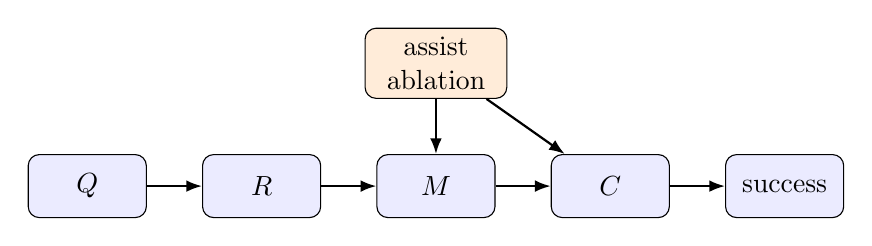
\begin{tikzpicture}[
    node distance=7mm and 7mm,
    box/.style={draw, rounded corners, align=center, minimum height=8mm, minimum width=15mm, fill=blue!8},
    arrow/.style={-{Latex[length=2.0mm]}, thick},
    assist/.style={draw, rounded corners, align=center, minimum height=7mm, minimum width=18mm, fill=orange!15}
  ]
    \node[box] (q) {$Q$};
    \node[box, right=of q] (r) {$R$};
    \node[box, right=of r] (m) {$M$};
    \node[box, right=of m] (c) {$C$};
    \node[box, right=of c] (s) {success};
    \node[assist, above=of m] (a) {assist\\ablation};
    \draw[arrow] (q) -- (r);
    \draw[arrow] (r) -- (m);
    \draw[arrow] (m) -- (c);
    \draw[arrow] (c) -- (s);
    \draw[arrow] (a) -- (m);
    \draw[arrow] (a) -- (c);
  \end{tikzpicture}
  \caption{Stage-structured interpretation of the Q/R/M/C framework. Assist on/off ablations target intermediate mechanisms; in the multi-agent extension the cadence protocol $\mathcal{C}_K$ acts on the R$\to$M and M$\to$C edges.}
  \label{p1:fig:causal}
\end{figure}

\paragraph{Relation to prior work.} Closest are (i) cognitive-map and semantic-map frameworks \citep{tolman1948cognitive,okeefe1978hippocampus,kuipers2000spatial,gupta2017cognitive,savinov2018semi}, (ii) goal-conditioned and successor-representation RL \citep{andrychowicz2017hindsight,ghosh2021learning,dayan1993improving,stachenfeld2017hippocampus,momennejad2017successor}, (iii) multi-agent communication \citep{lowe2017maddpg,foerster2018ctde,sukhbaatar2016commnet,foerster2016learning} and gossip/consensus \citep{boyd2006gossip,xiao2007distributed}, and (iv) LLM-agent memory layers evaluated end-to-end \citep{wang2023voyager,shinn2023reflexion,packer2023memgpt}. Our framework is orthogonal to all four: it \emph{diagnoses} where in the Q/R/M/C chain a given architecture succeeds or fails and lifts the cadence axis from network protocols to a cognitive-architecture parameter (full discussion in Appendix~\ref{p1:app:related-work-extended}).

\subsection{Event semantics, bounded rationality, and an order-theoretic reading}
\label{p1:sec:event-semantics}

The four starred events anchor at concrete logged triggers. We state the triggers once, because every empirical claim in the paper is a claim about them (per-regime formal definitions in Appendix~\ref{p1:app:estimators}), and we give each stage its reading in terms of the resource it bounds.

\begin{description}[leftmargin=10pt,topsep=2pt,itemsep=2pt]
\item[$Q^\star$ (intent issued).] The planner emits a semantic intent $q=(q^{\mathrm{req}},q^{\mathrm{pref}},q^{\mathrm{pen}})$: small sets of required, preferred, and penalty tags. The event is \emph{query emission}, not retrieval outcome: it fires when a valid query object is issued, so it is saturated whenever the task is semantic ($\hat P(Q^\star){=}1.00$ in Table~\ref{p1:tab:consistency}). A saturated stage is itself a diagnostic result --- it certifies that no failure mass sits at query formation. The multi-agent per-tick logger instruments the first \emph{retrieval} sub-event (a non-empty candidate set, $r^{\mathrm{set}}$) under the label $Q$ for historical reasons; since queries are emitted at every tick by construction there, the conditional rates are unchanged, but we record the relabeling explicitly (Appendix~\ref{p1:app:multi-agent-defs}). Resource bound: attention --- the intent is a few tags, not the full state.
\item[$R^\star$ (memory answers).] Retrieval evaluates $q$ against the memory and returns a candidate set. Two layers must be kept apart. \emph{Agent-side satisfaction} ($r^{\mathrm{set}}$): the set contains a record satisfying the query predicate --- the agent can verify this internally. \emph{Evaluator-side correctness} ($R^\star$): a retrieved candidate corresponds to a true satisfying place, verified through the \textbf{evaluation correspondence} $\Gamma \subseteq \mathcal{M} \times \mathcal{W}$ between memory records and world entities --- in our instrumented environments, $\Gamma$ is realised as spatial proximity ($\|c - w\| \le \epsilon$) to a ground-truth target, which only the evaluator can check. $R^\star$ as reported everywhere in this paper is the evaluator-side event. $\Gamma$ is part of the measurement contract: applying Q/R/M/C to a new substrate requires an explicit correspondence between internal referents and world entities, and errors in $\Gamma$ propagate to $R$ and $M$ (\S\ref{p1:sec:limitations}). The 91\% empty-candidate-set failures of \S\ref{p1:sec:refined-attribution} are \emph{logged} as $r^{\mathrm{set}}$-side events; the oracle ladder of Appendix~\ref{p1:app:oracle-ladder} shows the label conflates genuine retrieval emptiness (goal-region) with phrase-graph grounding failures recorded under the same taxonomy entry (hazard recovery). Resource bound: memory --- retrieval can only surface what consolidation has stored.
\item[$M^\star$ (target lock).] The planner materializes one candidate into a concrete actionable cell. Candidacy itself is threshold-gated (a place enters the candidate set only if its score clears the planner's gate, Appendix~\ref{p1:app:schemas}), and the lock commits to a single candidate once per query rather than re-optimizing against the full memory at every tick. The event fires on lock acquisition (correct under $\Gamma$, i.e.\ within $\epsilon$ of a true target, in the multi-agent logger). Resource bound: deliberation.
\item[$C^\star$ (closed-loop completion).] The local controller executes until the locked cell is reached or the episode times out; the event fires on arrival. $C$ is the only stage whose failure modes are extra-semantic: controller competence and, in the multi-agent regime, occupancy $\mathcal{O}_{-i}$. Resource bound: control, and in a collective, shared targets.
\end{description}

\paragraph{Observable-interaction reading.} The four events admit a
uniform reading as semantically distinct acts in the externally
observable interaction, with no reference to internal computational
state: $Q^\star$ is an informational commitment (a query stating what
evidence is needed); $R^\star$ is the memory's answer to that
commitment; $M^\star$ is a public commitment to act on specific
evidence, existing exactly from the moment the lock is written ---
and, in a collective, visible to peers and occupying a target;
$C^\star$ is the environment's confirmation that the commitment was
realized. This grounds Materialization independently of any cognitive
interpretation (the appearance of a public commitment is an objective
log event), and such commitments are the source of the
occupancy contention of \S\ref{p1:sec:multi-agent-results}. The stance
mirrors runtime verification and distributed-system observability,
where specifications constrain externally visible events rather than
internal state \citep{leucker2009runtime}.

\paragraph{Interpretive readings (all deferred).} The stages admit
three readings, none of which is a contribution and all of which now
live in the appendices: the pipeline as a \emph{satisficing, boundedly
rational} agent whose four resource bounds (attention, memory,
deliberation, control) are exactly the four failure loci
(Appendix~\ref{p1:app:hmdp}); an \emph{order-theoretic} account of empty
retrieval --- the $91\%$ regime --- via the query--extent Galois
connection (Appendix~\ref{p1:app:galois}); and an \emph{options/semi-MDP}
account of why optima appear on time-bearing metrics rather than on
the duration-blind chain probability $\Phi$
(Appendix~\ref{p1:app:hmdp}).

\section{Single agent: stage diagnostics localize failure}
\label{p1:sec:single}

\begin{table*}[t]
  \caption{System classes on which the Q/R/M/C contract is evaluated, and where each is reported. The single symbolic agent is the first row; the communicating collective, the learned-communication policies, and the local LLM agents are rows two to four (all instrumented within \S\ref{p1:sec:multi}); the three third-party agent stacks are the last row. ``Stage observability'' records whether the four conditional rates separate: full where an explicit query/lock interface exists, collapsed where a learned channel removes it, and marginal (non-nested event frequencies $f(\cdot)$) where only a tool trace is available.}
  \label{p1:tab:portability}
  \centering
  \small
  \begin{tabular}{p{3.5cm} p{4.6cm} p{3.5cm} c}
    \toprule
    System class & Representative instances & Stage observability & Section \\
    \midrule
    Single symbolic agent & node / concept / state-conditioned stack, four task families & full Q/R/M/C, oracle-testable & \S\ref{p1:sec:single} \\
    Multi-agent symbolic memory & independent / shared bus / central aggregator / peer($K$) & full Q/R/M/C per agent & \S\ref{p1:sec:multi} \\
    Learned communication & CommNet (REINFORCE/PPO), MAPPO & $Q$ saturates, R/M collapse & \S\ref{p1:sec:multi-agent-results} \\
    Local LLM agents & qwen3:4b, llama3.1, Qwen2.5-3B/7B (TextNav) & full; budget$\to$C, capability$\to$R & \S\ref{p1:sec:multi-agent-results} \\
    Third-party agent stacks & OpenAI SDK, LangGraph, AutoGen & marginal frequencies $f(\cdot)$, not nested & \S\ref{p1:sec:external} \\
    \bottomrule
  \end{tabular}
\end{table*}

This section instantiates the first row of
Table~\ref{p1:tab:portability}: a single symbolic agent, the simplest
system class, where the question is whether stage attribution adds
information that end-to-end success does not.

\subsection{System, tasks, and protocol}
\label{p1:sec:single-setup}

\paragraph{Memory stack.}
The system uses a graph substrate with a semantic retrieval interface on top: observations $o_t$ are tokenized into symbolic scene tokens and semantic tags that update a memory of place records, transitions, episodic traces, and concept/relation records. Planner queries return candidates by a weighted log-score over required, preferred, and penalty tags. The retrieval machinery is reused across all tasks and architectures; full memory schema, update rules, and scoring formula are in Appendix~\ref{p1:app:schemas}.

\paragraph{Tasks, baselines, protocol.}
Four single-agent task families are evaluated (water, safe-rest, goal-region on Empty-6x6 / FourRooms~\citep{sutton1999between}, hazard recovery on LavaGapS7), 10 seeds $\times$ 8 episodes each, $\times$ 2 assist modes. Semantic stack (node, concept, state-conditioned variants) is compared against four baselines: random, graph-only, SPTM-like, learned BC. Reported: end-to-end success, steps, four operational stage rates, assist deltas, weakest stage per task and per method. All means are seed-aggregated; 95\% bootstrap CIs use $B{=}5{,}000$ resamples~\citep{efron1979bootstrap}; assist comparisons use paired Wilcoxon signed-rank tests~\citep{wilcoxon1945individual} with Holm-Bonferroni correction~\citep{holm1979simple} (Appendix~\ref{p1:app:assist}). For the two hardest tasks (FourRooms, LavaGapS7), four oracle regimes (\emph{base}, \emph{oracle R/M/C}) are run — each replaces exactly one stage while leaving the rest of the pipeline unchanged. BabyAI portability check in Appendix~\ref{p1:app:babyai}. All single-agent experiments ran on a 10-core ARM CPU, 32\,GB RAM (CPU-only); oracle sweep $<1$\,min wall-clock.

\paragraph{LLM diagnostic block.}
To check that Q/R/M/C is not tied to the symbolic planner implementation, we also run a fixed TextNav substrate with an LLM-driven observe/query/retrieve/decide loop. The TextNav task, prompts, parser contract, and event definitions are held fixed while only the local Ollama model changes; the backend uses model-compatible completion settings when an Ollama chat template otherwise hides short structured answers in a separate thinking field. This block is a controlled step-budget study (Table~\ref{p1:tab:llm-smoke}): sweeping the completion budget drives both LLM agents into a failure that Q/R/M/C localizes to the $C$ stage while $Q/R/M$ stay saturated, exhibiting the framework's diagnostic property on real language agents. Reproducing full ReAct/Reflexion/Voyager/MemGPT-style agents is a separate systems contribution; the comparison to those systems is a coverage comparison in Appendix~\ref{p1:app:sota-coverage}.

\subsection{Stage-estimator validation}
\label{p1:sec:validation}

Before the main benchmark, the factorization is validated. On a
synthetic four-stage process with known probabilities the
nested-estimator product tracks empirical semantic-path completion
across sample sizes. On the real benchmark, the same product matches
semantic-path completion rather than overall success
(Table~\ref{p1:tab:consistency}) --- exactly the contract of
Propositions~1--2.

\begin{table*}[t]
  \caption{Stage-factor consistency audit for the best semantic method in each task family. The product of nested conditional estimators matches semantic-path completion; overall success can be higher because some episodes succeed without traversing the full semantic retrieval path.}
  \label{p1:tab:consistency}
  \centering
  \small
  \begin{tabular}{p{1.7cm}p{2.5cm}c c c c c c c}
    \toprule
    Task & Method & Overall & SP-comp & $\hat P(Q^\star)$ & $\hat P(R^\star|Q^\star)$ & $\hat P(M^\star|R^\star)$ & $\hat P(C^\star|M^\star)$ & Product \\
    \midrule
    Water & \texttt{water-cp} & 0.95 & 0.70 & 1.00 & 0.98 & 0.74 & 0.97 & 0.70 \\
    Rest & \texttt{rest-s2} & 0.93 & 0.73 & 1.00 & 1.00 & 0.80 & 0.91 & 0.73 \\
    Goal region & \texttt{goal-n1} & 0.54 & 0.00 & 1.00 & 0.54 & 0.01 & 0.00 & 0.00 \\
    Hazard recovery & \texttt{hazard-s7} & 0.40 & 0.16 & 1.00 & 0.56 & 0.58 & 0.50 & 0.16 \\
    \bottomrule
  \end{tabular}
\end{table*}

\subsection{Success-only summary and what it hides}
\label{p1:sec:single-results}

Water and rest are strong end-to-end tasks (0.95 and 0.93 success; Figure~\ref{p1:fig:hero}b). Goal-region reaches 0.54 success at the task-family level --- an average that pools a solved environment (Empty-6x6, $1.00$) with a hard one (FourRooms, $0.075$; \S\ref{p1:sec:oracle}), so the family number is bimodal rather than a uniform mid-difficulty --- but the bottleneck sits downstream of candidate selection (\S\ref{p1:sec:oracle}). Hazard recovery is the hardest retrieval-sensitive task at 0.40 success, with retrieval satisfaction as the weakest stage. Under success-only evaluation the two hard families look like the same kind of weakness; the stage view will show they are opposites. Per-task operational rates with 95\% CIs are in Table~\ref{p1:tab:main-results} (Appendix~\ref{p1:app:single-results-table}).

\paragraph{Baseline comparison.}
Table~\ref{p1:tab:baselines} compares the semantic stack against random,
graph-only, SPTM-like, and learned behavior-cloned baselines. The
learned baseline dominates the easiest resource tasks (1.00 on water
and rest) and hazard recovery (0.74), while the semantic stack remains
strongest on the relation-heavy goal-region family (0.54). The
relevant contrast for this paper, however, is not the success column:
the semantic stack is the only method family whose decisions expose
interpretable Q/R/M/C structure. On the BC baseline the stage events
are degenerate for the same structural reason as on the multi-agent
learned baseline analysed in \S\ref{p1:sec:multi-agent-results} --- a
policy without an explicit query/lock interface cannot emit separable
stage events, so the diagnostic decomposition has nothing to attach
to. End-to-end learning and stage diagnostics answer different
questions; this paper is about the second.

\begin{table*}[t]
  \caption{Baseline comparison. The learned behavior-cloned baseline dominates the easiest resource tasks and hazard recovery, while the semantic stack remains strongest on the relation-heavy goal-region family and remains the only family with interpretable Q/R/M/C structure.}
  \label{p1:tab:baselines}
  \centering
  \small
  \begin{tabular}{p{1.9cm}c c c c c}
    \toprule
    Task & Random & Graph-only & SPTM-like & Learned & Best semantic \\
    \midrule
    Water & 0.85 & 0.90 & 0.90 & 1.00 & 0.95 \\
    Rest & 0.85 & 0.90 & 0.90 & 1.00 & 0.93 \\
    Goal region & 0.41 & 0.49 & 0.52 & 0.50 & 0.54 \\
    Hazard recovery & 0.08 & 0.39 & 0.00 & 0.74 & 0.40 \\
    \bottomrule
  \end{tabular}
\end{table*}

\subsection{Oracle-stage interventions localize the bottleneck}
\label{p1:sec:oracle}

On goal-region the semantic variants solve Empty-6x6 ($1.00$ success) but collapse on FourRooms ($0.075$). For hazard recovery (LavaGapS7), base success $0.39$ (bootstrap 95\% CI $[0.35,0.43]$) rises only to $0.43$ under oracle controller, but jumps to $0.59$ under oracle materialization and $0.60$ under oracle retrieval (CI $[0.51,0.69]$; per-seed paired deltas positive in $9/10$ seeds, exact sign test $p{=}0.004$); goal-region rejoin is downstream-limited (oracle R lifts semantic-path completion to $0.08$ without moving end-to-end success). The per-task attribution as a stacked waterfall is in Figure~\ref{p1:fig:oracle-waterfall} (Appendix~\ref{p1:app:single-results-table}). Two tasks identical under success-only evaluation fail at opposite ends of the Q/R/M/C chain.

\paragraph{What an oracle intervention estimates.} Replacing a module changes everything downstream of it --- the visited state distribution, commitment times, subsequent memory accumulation, and the inputs the controller sees. An oracle contrast therefore estimates the \emph{total system-level effect} of replacing that module under the registered interface, $\mathbb{E}[Y^{do(R=\text{oracle})}] - \mathbb{E}[Y]$, not a surgical natural indirect effect through the stage event alone; Q/R/M/C is not a substitute for causal mediation analysis. Accordingly, ``retrieval-limited'' is used throughout in the operational sense: a task is \emph{retrieval-sensitive} when replacing retrieval (or materialization) under the registered interface produces a substantially larger success gain than replacing the downstream controller --- which is exactly the observed pattern on hazard recovery ($+0.21$/$+0.20$ vs $+0.04$ over the $0.39$ base) and its reverse on goal-region rejoin. Each oracle's replacement boundary (what is substituted, what remains native, and what hidden state it may read) is specified in Appendix~\ref{p1:app:oracle-c-def}.

\subsection{The logs refine the diagnosis: a candidate-availability limit}
\label{p1:sec:refined-attribution}

Inspecting the framework's own logs sharpens the retrieval attribution. On the 10-seed hazard-recovery run, $349$ retrieval calls were logged: only $32$ ($9.2\%$) returned at least one candidate, and of these $31$ ($96.9\%$ precision) selected a semantically satisfied candidate. The bottleneck is therefore not candidate \emph{ranking} but candidate \emph{availability} --- the symbolic memory does not contain hazard-recovery-tagged nodes at 91\% of decision points. A retrained 2-layer candidate-generation MLP trained on per-state features (test accuracy $0.59$ vs majority-class $0.81$; Appendix~\ref{p1:app:learned-baselines}) confirms that instantaneous state features cannot substitute for the missing structure. The framework's ``retrieval-limited'' attribution thus refines to a \emph{candidate-availability} limit. A stage-wise oracle ladder (Appendix~\ref{p1:app:oracle-ladder}) then separates the upstream causes along the perception $\to$ write $\to$ consolidation $\to$ grounding path, with a result that corrects our own initial reading. On hazard recovery the absences are predominantly \emph{grounding} failures, not storage failures: separate instrumentation shows the retrieval stage internally returns at least one candidate on $0.90$ of calls, but the planner fails to ground a path to it in the phrase graph on $0.80$ of calls --- and that grounding failure was logged as an empty candidate set. An oracle that writes ground-truth semantic tags at every observation changes nothing (perception and write are not the cause); oracles that bypass phrase-graph grounding (direct waypoint from the retrieved candidate, or from perfect raw history) eliminate the empty-set symptom almost entirely ($0.45 \to 0.05$ per-episode; per-query non-emptiness $0.11 \to 0.87$) yet do \emph{not} raise success ($0.36$ vs.\ $0.39$ base, CIs overlapping) --- whereas oracle retrieval raises success by $+0.21$. The binding constraint on this task is therefore the semantic \emph{quality} of the candidates the memory designates, not their availability. On goal-region the decomposition is different: there the retrieval stage itself is empty on $0.70$ of calls (genuine coverage-driven emptiness), and even oracle retrieval does not move end-to-end success, placing the constraint downstream in exploration and control. The taxonomy label ``empty candidate set'' thus conflated two mechanisms that the ladder now separates per task; what the original evidence correctly excluded --- and the ladder confirms --- is ranking, thresholding, and perception. This attribution is not an artefact of the required-tag threshold $\theta$: sweeping $\theta$ across the full range leaves the empty-candidate-set rate invariant (Appendix~\ref{p1:app:theta-robustness}), because the empties are absence of any stored candidate, not sub-threshold filtering. Nor is it an artefact of the weighting: the empty rate is $0.908$ pooled over calls, $0.909$ seed-weighted, and $0.891$ episode-weighted (mean over the 80 episodes of each episode's own empty share), so long failing episodes contributing more decision points do not inflate the figure. Accumulation itself is not one of the four stages: the protocol localized the failure to the R link, and this within-link forensics named the cause --- we read Q/R/M/C as coarse localisation with a designated drill-down, not as a complete causal ontology of memory failure. This sets up the multi-agent section: when consolidation becomes a shared process across $N$ agents, it acquires a measurable \emph{rate}.

\section{Multi-agent: memory as a shared resource}
\label{p1:sec:multi}

This section instantiates rows two to four of
Table~\ref{p1:tab:portability}: the same logged events, unchanged,
instrument a communicating collective --- and, within the same
section, learned policies and LLM agents --- where the additional
failure axis is contention for the targets that memory designates.

\subsection{Four memory architectures and the cadence axis}
\label{p1:sec:archs}

Four communication architectures are instantiated; they share the
single-agent retrieval substrate but differ in how memory is
distributed across agents (Figure~\ref{p1:fig:architectures}).

\begin{figure}[t]
  \centering
  
\includegraphics[width=\linewidth]{figures/fig_architectures.pdf}
  \caption{Four multi-agent memory architectures. \textbf{(a)} Independent: per-agent private memory, no exchange. \textbf{(b)} Shared bus: one global memory, every agent reads/writes each tick. \textbf{(c)} Central aggregator: per-agent memories plus a hub that merges them into a consensus report. \textbf{(d)} Peer-to-peer broadcast: per-agent memories with pairwise snapshot exchange every $K$ ticks (the cadence axis of Empirical Claim~1).}
  \label{p1:fig:architectures}
\end{figure}

\begin{description}[leftmargin=10pt,topsep=2pt,itemsep=2pt]
\item[Independent.] Each agent maintains a private event store and concept graph. No inter-agent communication mechanism exists. Lower-bound baseline.
\item[Shared bus.] All agents publish observations to a single \emph{collective memory} event bus. One shared concept graph is rebuilt from the union of events. Maximally centralized.
\item[Central aggregator (ConsensusLayer).] Each agent has its own private concept graph; a central layer pulls snapshots and computes a trust-weighted merge, producing a single \emph{consensus report} consumed by all agents.
\item[Peer-to-peer broadcast (cadence $K$).] Each agent has its own concept graph and its own merged view. Every $K$ ticks each agent broadcasts a snapshot to a passive bus; each agent independently merges its own snapshot with the latest snapshot received from each peer. Different agents may hold different merged views; there is no central report.
\end{description}

The first three correspond to the three regimes in the multi-agent
communication literature: no exchange, CTDE-style aggregation, and
decentralized peer communication. The fourth is the architecture for
which Definition~2 and Empirical Claim~1 are directly
applicable, since the cadence $K$ is a tunable parameter rather than a
fixed protocol. Mechanically, $K$ is the rate at which private
memories consolidate into a collective view, which is why it is the
structural axis of this section.

\subsection{Multi-agent factorization}
\label{p1:sec:multi-theory}

Extend the factorization to a population of $N$ agents that share
information through a communication protocol $\mathcal{C}_K$
parameterized by broadcast cadence $K$. Each agent $i$ has its own
memory state $\mathcal{M}_i$ and issues its own query $q_i$. Let
$\mathcal{M}_i^{(K)}$ denote the projection of agent $i$'s memory at
the moment it queries, after absorbing every peer message received
under cadence $K$. Two coupling channels are separated: (i) memory
coupling $\mathcal{M}_{-i}^{(K)}$, the latest peer memory snapshots
accessible to agent $i$; (ii) occupancy coupling $\mathcal{O}_{-i}$,
the set of targets that other agents have already claimed by the time
$i$ acts.

\paragraph{Definition 2 (multi-agent stage decomposition).}
For each agent $i$, the per-agent starred events remain nested, so
Proposition~1 applies verbatim:
\[
P(C^\star_i)
=
P(Q^\star_i)\,
P(R^\star_i \mid Q^\star_i)\,
P(M^\star_i \mid R^\star_i)\,
P(C^\star_i \mid M^\star_i),
\]
identically, with no assumption; and the estimators are consistent
under the conditions of Proposition~2, with the cluster structure now
including agents within a shared world realization. What is new in the
multi-agent setting is the \emph{structural} reading: interpreting
$P(M^\star_i|R^\star_i)$ as a property of agent $i$'s materialization
mechanism requires that dependence on past peer decisions enter only
through the logged couplings --- $\mathcal{M}_{-i}^{(K)}$ at the
R$\to$M edge and $\mathcal{O}_{-i}$ at the M$\to$C edge.

\paragraph{When the structural reading of Definition~2 may fail.}
The single-agent structural assumption absorbs trajectory history into
the logged $(q, \mathcal{M})$. In the multi-agent setting, the
analogous absorption is non-trivial: $\mathcal{O}_{-i}$ summarises
target occupancy at decision time but loses information about
\emph{how} peers arrived there. The mechanism-level reading is
therefore a projection onto observable per-agent traces under that
summary; the descriptive factorization above is unaffected. Two
specific failure modes arise: (i) inter-agent communication
side-channels not logged through $\mathcal{C}_K$; (ii) coordinated
peer policies whose decision at the C stage depends on hidden peer
state not summarised by $\mathcal{O}_{-i}$.

\subsection{Bottleneck shift}
\label{p1:sec:shift}

\paragraph{Empirical Claim~1 (bottleneck shift M$\leftrightarrow$C, slope-level).}
Assume scarcity ($N > T$ targets, see \S\ref{p1:sec:notation}) and a
peer-broadcast architecture with cadence $K \in \mathbb{N}$. Two
stylized assumptions are posited:
\textbf{(F)} memory freshness $\nu(\mathcal{M}_{-i}^{(K)})$ is
non-decreasing pointwise as $K$ decreases, and the probability that
agent $i$'s planner locks onto a reachable target is non-decreasing in
$\nu$;
\textbf{(O)} the probability that an arbitrary committed target is
already in $\mathcal{O}_{-i}$ is non-increasing as $K$ increases.
Write $P(M^\star|R^\star;K)$ and $P(C^\star|M^\star;K)$ for the
population-level conditional probabilities (averaged over agents and
the seed distribution of the benchmark); $\hat{P}(\cdot)$ denotes the
corresponding empirical-frequency estimator computed from logs. Under
(F) and (O),
\[
\frac{\partial\, P(M^\star|R^\star;K)}{\partial K^{-1}} > 0,
\qquad
\frac{\partial\, P(C^\star|M^\star;K)}{\partial K^{-1}} < 0.
\]
Both slope conditions are direct empirical predictions that are
testable on logs through $\hat{P}$.

\paragraph{What this claim is and is not.}
Empirical Claim~1 is a \emph{slope-level statement on conditional rates}: each of the two slopes is testable and is confirmed on the 35{,}640-run sweep (\S\ref{p1:sec:multi-agent-results}) and independently on a 100-run standard-MiniGrid portability sweep (\S\ref{p1:sec:limitations}). We report the slopes as \emph{effect sizes with cluster-robust confidence intervals} (resampled over the 81 independent configuration cells rather than the correlated run count) in Appendix~\ref{p1:app:effect-sizes}. The claim's boundary with respect to the conditional product $\Phi$ is stated once, in the Scope-and-non-claims box (\S1) and in \S\ref{p1:sec:multi-agent-results}. The shift is a signature of scarce-target contention, not of the grid design: under abundance ($T{>}N$) both slopes flatten and the M$\leftrightarrow$C anticorrelation attenuates (Appendix~\ref{p1:app:cadence-robustness}), i.e.\ the prediction breaks exactly where the contention mechanism is removed.

\paragraph{Chronology.}
Empirical Claim~1 is post-hoc. It was formulated \emph{after} an initial 12{,}960-run sweep conducted under four stage-agnostic hypotheses (Appendix~\ref{p1:app:diagnostics}); the two slope conditions were then confirmed on the full 35{,}640-run sweep, on the $N\!=\!12$ scale-up (Appendix~\ref{p1:app:babyai}), and on the MiniGrid portability wrapper (\S\ref{p1:sec:limitations}). We state this explicitly: the verified slope signs are predictions on enlarged data, not a pre-registered (externally timestamped)
prediction. A fully formal version is left for future work.

\subsection{Sweep protocol}
\label{p1:sec:multi-agent-protocol}

The four architectures are evaluated on a custom multi-agent grid ($12{\times}10$ cells); each agent must reach a cell tagged \texttt{water\_source}, choosing actions via a shared memory-driven planner so only the memory layer differs. The sweep crosses $N{\in}\{3,5,8\}$, $T{\le}N$, three layouts (symmetric/asymmetric/random), three hazard densities, four architectures, eight peer cadences $K{\in}\{1,2,4,8,16,32,48,64\}$, 40 seeds --- 35{,}640 runs in $\approx 22$ min on 8 cores. Per-agent per-tick Q/R/M/C indicators are logged (Appendix~\ref{p1:app:estimators}); episode-level starred events are the disjunction over ticks. A separate oracle-intervention block on scarcity cases $(N,T){\in}\{(3,2),(5,3),(8,5)\}$ at five cadences evaluates oracle R (memory returns ground-truth water positions), oracle M (planner locks onto nearest real water), and oracle C (completion of a real materialized lock is guaranteed; Appendix~\ref{p1:app:oracle-c-def}).

\subsection{Results: stage decomposition and bottleneck shift}
\label{p1:sec:multi-agent-results}

The 35{,}640-run sweep is reported through four observations,
structured to mirror Empirical Claim~1: (i) the conditional
decomposition isolates the M and C stages as the differentiating
links; (ii) the bottleneck shift appears directly as a negative
within-cadence correlation between $P(M^\star|R^\star)$ and
$P(C^\star|M^\star)$, peaking at $K\!=\!4$ and decaying to noise at
$K\!=\!64$; (iii) on mean time-to-success, the resulting trade-off
produces an interior optimum at $K\!=\!8$ --- robust in location but shallow in margin, with the advantage over the adjacent fast cadences not resolved at this sample size (Appendix~\ref{p1:app:effect-sizes}); (iv) on the
conditional product $\Phi$, the same trade-off produces a monotone
trend rather than an interior peak --- a summary statistic on which we make no formal claim. A learned-communication baseline and a multi-agent
oracle-intervention loop close the subsection.

\subsubsection{Conditional decomposition reveals where each architecture fails.}
Figure~\ref{p1:fig:conditional-rates} shows per-architecture conditional Q/R/M/C rates; full numerics with bootstrap CIs are in Appendix~\ref{p1:app:phi-detail}, Table~\ref{p1:tab:multi-agent-cond}. Retrieval conditional $P(R^\star|Q^\star)$ is saturated; the differentiating signal lives at M and C. Shared-bus, central-aggregator, and fast-broadcast peer ($K\le4$) have high $P(M^\star|R^\star)$ but low $P(C^\star|M^\star)$; independent and slow-broadcast peer ($K\ge16$) show the reverse --- the M$\leftrightarrow$C trade-off predicted by Empirical Claim~1.

\begin{figure}[t]
  \centering
  
\includegraphics[width=\linewidth]{figures/fig_conditional_rates.pdf}
  \caption{Per-architecture conditional rates (top) and mean time-to-success among successes (bottom) from the 35{,}640-run sweep. Error bars and band: 95\% cluster-bootstrap CIs over the 81 design cells; points are cell-weighted means ($7.63$ at $K{=}8$ vs.\ $8.04$ independent; the run-pooled values of Table~\ref{p1:tab:multi-agent-cond} are $7.47$/$8.02$). Shared bus, central aggregator, and fast peer broadcast ($K \le 4$) live in the M-saturation / C-collapse regime; independent and slow peer ($K \ge 16$) live in the M-deficit / C-saturation regime. The interior minimum at $K{=}8$ is robust in location but shallow in margin (Appendix~\ref{p1:app:effect-sizes}); the censoring-aware contrast is in the text.}
  \label{p1:fig:conditional-rates}
\end{figure}


\subsubsection{Bottleneck shift and interior efficiency optimum.}
Across all peer runs, Spearman of $P(M^\star|R^\star)$ vs $K$ is $-0.53$ (95\% cluster-robust CI $[-0.59,-0.47]$) and of $P(C^\star|M^\star)$ vs $K$ is $+0.43$ (CI $[+0.37,+0.50]$); both are moderate effect sizes whose CIs exclude zero under resampling of the 81 configuration cells (Appendix~\ref{p1:app:effect-sizes}), matching the slope conditions of Empirical Claim~1. We report these rather than $p$-values, which are uninformative at this correlated sample size. Both slope signs are also robust to the two free thresholds of the logger --- candidacy $\theta$ and lock tolerance $\epsilon$ (Appendix~\ref{p1:app:theta-robustness}). The stronger empirical signature is at the per-configuration level: Pearson of $P(M^\star|R^\star)$ vs $P(C^\star|M^\star)$ \emph{within} a fixed $K$ is $-0.43, -0.54, -0.61, -0.19, -0.05, -0.04, -0.02, -0.02$ at $K{=}1,2,4,8,16,32,48,64$, peaking at $K{=}4$ and decaying to noise by $K{=}64$ (Figure~\ref{p1:fig:jensen-scatter}, Appendix~\ref{p1:app:phi-detail}). Configurations where M is high systematically have low C: the bottleneck migrates between the two stages within the same $(N,T,\text{layout},\text{hazard},\text{seed})$ cell as $K$ varies. On the efficiency metric, mean $t_{\mathrm{succ}}$ has a U-shape with interior minimum at $K{=}8$ (7.47 ticks vs 8.02 for the independent baseline); the minimum's location is robust but shallow --- its margin over the adjacent fast cadences ($K{=}1,4$) is not resolved under cell-level resampling (paired-bootstrap CIs in Appendices~\ref{p1:app:phi-detail} and \ref{p1:app:effect-sizes}). Both statements condition on success. Under a censoring-aware expected time that charges failed runs the full step limit, the fast flank reverses and the independent baseline is marginally best (cell-paired $\Delta(K{=}8-\text{independent}) = +0.32$, CI $[+0.05,+0.63]$; Appendix~\ref{p1:app:effect-sizes}): at fast cadence the completion decline reduces the success rate by more than the materialization gain increases it, so the interior optimum is a statement about conditional speed, not unconditional efficiency --- and closing the unconditional gap is what the reservation-and-rollback protocol (companion route-transfer study \citep{songlines2}) achieves (Appendix~\ref{p1:app:open-problems}). Scaling to $N{=}12$ \emph{sharpens} the signature: the peak Pearson rises to $-0.70$ and
migrates outward to $K\!=\!8$, consistent with stronger occupancy
coupling at higher $N$ delaying the cost-regime transition
(Appendix~\ref{p1:app:babyai}, Figure~\ref{p1:fig:scale-n12}).

\paragraph{Provenance stratification: the mechanism behind the shift.}
Annotating each $M^\star$ lock with the \emph{provenance} of the
evidence behind it makes the bottleneck shift mechanistic rather than
correlational. Let $\varphi$ be the foreign share of the evidence mass
supporting the locked candidate, computed from the same trust/support
weights the merge itself used and frozen at lock time, and call a lock
a \emph{warp} ($W^\star$) when $\varphi \ge 0.8$: the agent is
committing to a target it knows essentially only from peers. On a
dedicated peer sweep over the scarcity cells (random layouts, 20
seeds, $K\in\{1,2,4,8,16\}$) the warp share $P(W^\star|M^\star)$
falls from $0.55$ at $K{=}1$ to $0.11$ at $K{=}8$ while the
own-evidence stratum completes at a flat $0.26$--$0.34$ and the warp
stratum completes below $0.05$ throughout: \emph{the C-collapse of
fast sharing is concentrated in the warp stratum}. What cadence
controls, mechanically, is how much of the collective's
materialization runs on foreign evidence --- and that is
the stratum whose completions are lost to occupancy contention. The stratification is not
an artefact of the $0.8$ cutoff: recomputed from the raw per-lock
$\varphi$ values ($23{,}237$ locks) at thresholds
$\varphi{\in}\{0.5,0.6,0.7,0.8,0.9,0.95\}$, the foreign stratum
completes at ${\le}0.03$ while the own stratum stays at
$0.26$--$0.50$, at every threshold and cadence. The two coupling
channels also separate interventionally with arms already in the
design: the independent arm removes peer evidence while leaving
target contention in place, and the reservation-and-rollback protocol
evaluated in the companion route-transfer study \citep{songlines2} keeps peer evidence
while managing contention --- under it, unconditional success at fast
cadence exceeds the $K{=}8$ baseline ($0.614$--$0.620$ vs.\
$0.583$; paired improvement over the same cells without the mechanism
$\Delta=+0.037$, cluster-bootstrap 95\% CI $[+0.018,+0.058]$ over 18
matched design cells), identifying occupancy contention rather than
evidence quality as the cost channel of fast sharing. The same stratification
reproduces on the continuous VMAS bridge ($0.72\to0.00$ over
$K{=}1/4/16$) and on an LLM text substrate ($0.42\to0.08$ over
$K{=}2/8$), with the curves nearly coinciding across substrates. A
full provenance-conditioned analysis (counterfactual attribution by
masked replay, a closed-form staleness horizon with a pre-specified
$6/6$-exact hold-out, and a decentralized repair protocol) appears in
a companion route-transfer study \citep{songlines2}; here the stratification serves as the
mechanistic reading of Empirical Claim~1.

\paragraph{What we do not claim about $\Phi$.} The conditional product $\Phi = P(M^\star|R^\star)\!\cdot\!P(C^\star|M^\star)$ does \emph{not} have an interior peak in the tested range (mean-of-products estimator increases monotonically from $0.569$ at $K{=}4$ to $0.603$ at $K{=}64$, converging to the independent-agent boundary $0.605$). The slope-level statement of Empirical Claim~1 is on the conditional rates themselves, not on $\Phi$; we make no formal claim about the shape of $\Phi(K)$. Jensen-gap detail and POM--MOP comparison in Appendix~\ref{p1:app:phi-detail}.

\paragraph{Learned-communication baseline: stage events are structurally degenerate even at competitive success.}
A CommNet-style policy \citep{sukhbaatar2016commnet} trained with PPO~\citep{schulman2017proximal} on the same scenario ($N{=}3$, $T{=}2$) reaches $0.667$ held-out success ($n{=}100$ seeds) --- matching the symbolic peer architecture at $K{=}8$ ($0.65$). Despite this, the Q/R/M/C profile remains structurally degenerate: $Q^\star{=}1.00$ saturated by construction; $R^\star{=}0.997$, $M^\star{=}0.997$ collapsed together ($P(M^\star|R^\star){=}1.00$). This is the verified structural claim, and it is a claim about the \emph{exposed interface}, not about the policy's internals: a real-valued comm vector is never informatively empty (Q saturates) and lacks an explicit target-lock interface, so R and M are not separately identifiable from the observable event mapping --- they collapse \emph{as logged events}. Whether functionally distinct retrieval- and commitment-like processes exist inside the learned policy is a separate question that this instrumentation cannot answer; probing hidden states for latent commitment times is the natural follow-up.

\paragraph{A learned agent \emph{with} the interface.} The converse experiment closes the objection that observability is an artefact of our symbolic design: a PPO-trained neural agent built \emph{around} explicit interfaces --- a query head emitting a discrete semantic query, a learned retriever scoring an append-only observation store (top-$4$), an explicit target-lock head committing one candidate to environment-visible state, and a learned controller --- trains to $0.665$--$0.666$ held-out success over $3$ seeds ($400$ PPO updates; artifact \texttt{tmp/cluster/neural\_explicit\_s*/}), matching both the CommNet baseline ($0.667$) and the symbolic peer at $K{=}8$ ($0.65$). Its Q/R/M/C events are separately logged and non-degenerate during training; the honest caveat is that at convergence the lock head follows top-$1$ retrieval in $98$--$99\%$ of commitments, so the R and M \emph{behaviors} become nearly deterministic even though the events remain separately observable --- observability is a property of the design, not a tax on performance, but an explicit interface does not by itself guarantee that the stages stay behaviorally distinct. The multi-agent counterpart of the single-agent learned-BC analysis (\S\ref{p1:sec:single-results}). Full architecture, PPO hyperparameters, and side-by-side REINFORCE vs PPO comparison in Appendix~\ref{p1:app:learned-baselines}.

\paragraph{LLM model sweep: the logger localizes a real failure in language agents.}
Table~\ref{p1:tab:llm-smoke} runs the same Q/R/M/C event contract on four LLM agents over two independent backends: qwen3:4b and llama3.1 via local Ollama ($8$ episodes/cell), and Qwen2.5-3B/7B-Instruct via HuggingFace transformers on SLURM GPU nodes ($25$ episodes/cell). The decomposition separates \emph{two different failure modes on two different stages}. \textbf{Budget $\to$ C:} below the task's step requirement, three models (qwen3:4b, llama3.1, Qwen2.5-7B) show the identical signature $Q^\star{=}R^\star{=}M^\star{=}1.00$, $C^\star{=}0.00$ --- a completion-limited failure that replicates across backends, model families, and hardware. \textbf{Capability $\to$ R:} Qwen2.5-3B fails at \emph{every} budget with $Q^\star{=}1.00$ but $R^\star{=}0.00$: it declares the target, emits well-formed actions (verified against the response cache, so not a parsing artifact), yet wanders without ever storing the evidence retrieval needs --- an exploration/grounding failure surfacing at the R stage, exactly the ``absence of evidence'' regime of \S\ref{p1:sec:refined-attribution}. An opaque scalar would report both models as $0.00$; the stage view shows they fail for different reasons at different stages. (Instrumentation note: a naive qwen3:4b/Ollama chat-template call initially returned empty \texttt{response} strings because the model spent the short structured-output budget in a separate thinking field; we use raw structured completion for qwen3:4b and a first-line parser, recorded for reproducibility.)

\paragraph{The multi-agent phenomenology reproduces on a live LLM collective.}
Beyond the single-agent budget study, the same event contract
instruments a collective of $N{=}3$ LLM agents (llama3.1) sharing
symbolic place memory by peer broadcast under scarcity ($M{=}2$
takeable targets, four layouts, $K\in\{2,8\}$), with all predictions
specified before the runs. The cadence phenomenology of
\S\ref{p1:sec:multi-agent-results} carries over to the language
substrate: a paired comparison against the no-communication baseline
on identical layouts shows raw sharing \emph{lowering} success from
$2/3$ to $1/3$ per episode --- the occupancy-racing C-collapse, now
produced by agents whose queries, tag extraction, and commitments are
LLM-made --- and target collisions appear in $7/8$ shared-memory
episodes. Attaching the reservation-and-rollback repair protocol
(Appendix~\ref{p1:app:open-problems}, evaluated independently in the
companion route-transfer study \citep{songlines2}) recovers part of the loss
($0.333\to0.417$ at both cadences, rollback latency again
${\approx}K$). Two interface findings transfer to any
LLM-over-symbolic-memory design: LLM query formers free-generate
retrieval tags outside the memory's vocabulary (requiring tolerant
retrieval gates), and small local models are reliable at semantic
commitment but not at coordinate arithmetic or systematic exploration
(requiring layered execution). Full protocol and provenance analysis
in the companion route-transfer study \citep{songlines2}.

Scope: these are controlled studies on local models; scaling the same contract to full Voyager/MemGPT-style agents on richer tasks with multiple failure modes is developed next (external-framework validation) and in Appendix~\ref{p1:app:sota-coverage}.

\begin{table}[h]
  \caption{LLM TextNav step-budget sweep across four models and two independent backends (local Ollama, $n{=}8$/cell; HuggingFace transformers on a SLURM GPU cluster, $n{=}25$/cell; temperature 0.0; the task needs $\sim$10 low-level steps). Two distinct failure modes are localized to two different stages. \textbf{Budget $\to$ C:} at step limit 6, qwen3:4b, llama3.1 and Qwen2.5-7B all show $Q^\star{=}R^\star{=}M^\star{=}1.00$ with $C^\star{=}0.00$ --- the completion-limited failure replicates across backends, models, and hardware. \textbf{Capability $\to$ R:} Qwen2.5-3B fails at \emph{every} budget ($\{6,8,12,25\}$) with $Q^\star{=}1.00$ but $R^\star{=}0.00$: it declares the target yet never accumulates the evidence to retrieve it (its outputs are well-formed action strings --- verified in the response cache --- so this is an exploration/grounding failure feeding retrieval, not a parsing artifact). Artifacts: \texttt{tmp/llm\_steplimit\_*}, \texttt{tmp/cluster/textnav*}.}
  \label{p1:tab:llm-smoke}
  \centering
  \small
  \begin{tabular}{l l c c c c c c}
    \toprule
    Model & Backend & Step limit & Success & $Q^\star$ & $R^\star$ & $M^\star$ & $C^\star$ \\
    \midrule
    qwen3:4b        & ollama & 6  & 0.00 & 1.00 & 1.00 & 1.00 & \textbf{0.00} \\
    llama3.1        & ollama & 6  & 0.00 & 1.00 & 1.00 & 1.00 & \textbf{0.00} \\
    Qwen2.5-7B      & hf     & 6  & 0.00 & 1.00 & 1.00 & 1.00 & \textbf{0.00} \\
    \midrule
    qwen3:4b        & ollama & 12 & 1.00 & 1.00 & 1.00 & 1.00 & 1.00 \\
    llama3.1        & ollama & 12 & 1.00 & 1.00 & 1.00 & 1.00 & 1.00 \\
    Qwen2.5-7B      & hf     & 12 & 1.00 & 1.00 & 1.00 & 1.00 & 1.00 \\
    \midrule
    Qwen2.5-3B      & hf     & 6--25 & 0.00 & 1.00 & \textbf{0.00} & 0.00 & 0.00 \\
    \bottomrule
  \end{tabular}
\end{table}

\paragraph{Multi-agent oracle interventions close the diagnose$\to$intervene$\to$verify loop.}
On the scarcity cases, mean $t_{\mathrm{succ}}$ at small/intermediate cadence ($K{\in}\{1,2,4\}$) drops from $\sim10$--$11$ in baseline to $\sim7.2$ under either oracle R or oracle M, and further to $\sim6.1$ under oracle C, which additionally removes post-lock travel; at slow cadence ($K{=}16$) the baseline is already within $\sim1.2$ of the R/M oracle floor (Table~\ref{p1:tab:multi-agent-oracle} in Appendix~\ref{p1:app:multi-oracle}). Crucially, oracle C gives the largest time reduction but the smallest success-rate gain (Appendix~\ref{p1:app:oracle-c-def}): in scarcity, completion costs time while retrieval and materialization decide success. The cadence-induced excess time at small/intermediate $K$ is attributable to the M$\leftrightarrow$C transition; at large $K$ the bottleneck has moved into solo exploration.

The multi-agent block thus delivers its half of the argument. The
cadence $K$ is, mechanically, the rate at which private memories
consolidate into a collective view; the data show that this rate has a
non-trivial interior optimum ($K\!=\!8$ on $t_{\mathrm{succ}}$), that
its cost channel is occupancy coupling, and that both effects are
visible stage-by-stage on the same Q/R/M/C chain used for single
agents. Consolidation is not only the single-agent limit; in a
collective it is a tunable, measurable design axis.

\section{The contract on third-party agent stacks}
\label{p1:sec:external}

This section instantiates the last row of
Table~\ref{p1:tab:portability}. We further evaluate the protocol on
systems built by others. The contract has two layers: an \emph{invariant core} --- four event
roles (a memory query is issued; returned evidence satisfies the
task; the agent commits to a target; the task completes) --- and a
\emph{system-specific adapter} that maps logged actions to those
roles. We instrument three third-party agent stacks --- a
function-calling loop on the OpenAI SDK, LangGraph's prebuilt ReAct
agent, and AutoGen's AssistantAgent/UserProxy pair, all driving the
same local model (llama3.1, temperature $0$) --- with one tool-trace
adapter shared by all three: an episodic household memory is exposed
through \method{recall}/\method{goto}/\method{take} tools, and
$Q^\star$ fires on querying memory, $R^\star$ on \emph{attribution}
(a returned record names the item at its true place), $M^\star$ on a
commitment (a \method{goto} to the true place; first-commitment
accuracy $M_1$ is logged as an auxiliary lock-quality diagnostic),
and $C^\star$ on task completion within a tool budget. A tool trace
exposes no lock chain, so these are \emph{marginal event frequencies}
$f(\cdot)$ in the sense of Appendix~\ref{p1:app:estimators}: an agent
can commit to the true place without a supporting retrieval, the
events are not nested, and no factorisation is claimed --- the four
frequencies serve as separate diagnostics and are never substituted
into the chain-rule product. What varies across system
classes is the adapter, not the event roles. Three variants engineer
one failure each --- a consolidation gap (the location fact was never
written to memory), a stale-distractor ambiguity, a tool budget below
the task's requirement --- plus a clean control; all predictions were
specified before the runs, and the two revisions of the adapter (an
attribution leak; an over-tightened $M^\star$) are recorded in the
registration file.

\begin{table}[h]
\caption{Marginal Q/R/M/C event frequencies on three third-party
agent frameworks (llama3.1, 20 episodes per cell, identical
episodes/tools/budgets). Each entry is the fraction of episodes in
which the event occurred: $Q^\star$ --- the agent queried memory at
least once; $R^\star$ --- a returned record named the item at its
true place; $M^\star$ --- the agent committed (\method{goto}) to the
true place, with or without retrieval support; $C^\star$ ---
\method{take} succeeded within the tool budget; $M_1$: first
\method{goto} targets the true place; stale$_1$: first \method{goto}
targets the stale distractor. The events are not nested and no
product is claimed (Appendix~\ref{p1:app:estimators}): under the
consolidation gap, budgeted blind search over the four places
sometimes commits to and reaches the true place, hence
$M^\star, C^\star > 0$ at $R^\star{=}0$. Structural failures localize
identically everywhere: the consolidation gap is $R^\star{=}0.00$ and
the budget failure is $C^\star{=}0.00$ at $Q^\star{=}R^\star{=}1$,
for all three stacks. On the \emph{clean} control the frameworks
spread from $0.50$ to $0.75$ end-to-end --- and the decomposition
attributes the spread (see text).}
\label{p1:tab:external}
\centering
\small
\begin{tabular}{llcccccc}
\toprule
Framework & Variant & $f(Q^\star)$ & $f(R^\star)$ & $f(M^\star)$ & $f(C^\star)$ & $f(M_1)$ & $f(\text{stale}_1)$ \\
\midrule
OpenAI SDK & control     & 1.00 & 1.00 & 0.85 & 0.75 & 0.25 & --- \\
           & consolidation gap & 1.00 & \textbf{0.00} & 0.50 & 0.40 & 0.25 & --- \\
           & stale ambiguity   & 1.00 & 1.00 & 0.90 & 0.30 & 0.25 & 0.20 \\
           & tight budget      & 1.00 & 1.00 & 0.25 & \textbf{0.00} & 0.25 & --- \\
\midrule
LangGraph  & control     & 1.00 & 1.00 & 0.70 & 0.50 & 0.50 & --- \\
           & consolidation gap & 1.00 & \textbf{0.00} & 0.20 & 0.15 & 0.10 & --- \\
           & stale ambiguity   & 1.00 & 1.00 & 0.65 & 0.60 & 0.50 & 0.35 \\
           & tight budget      & 1.00 & 1.00 & 0.10 & \textbf{0.00} & 0.10 & --- \\
\midrule
AutoGen    & control     & 1.00 & 1.00 & 0.85 & 0.55 & 0.45 & --- \\
           & consolidation gap & 1.00 & \textbf{0.00} & 0.30 & 0.20 & 0.15 & --- \\
           & stale ambiguity   & 1.00 & 1.00 & 0.50 & 0.45 & 0.35 & 0.40 \\
           & tight budget      & 1.00 & 1.00 & 0.15 & \textbf{0.00} & 0.15 & --- \\
\bottomrule
\end{tabular}
\end{table}

\begin{figure}[t]
\centering

\includegraphics[width=\linewidth]{figures/fig_external_stages}
\caption{Stage profiles of three third-party agent stacks on the four
engineered variants (llama3.1, $n{=}20$ per cell). Query and retrieval
saturate identically everywhere; the two structural failures produce
exact zero columns on every stack ($R^\star{=}0$ under the
consolidation gap, $C^\star{=}0$ under the tight budget); the
behavioral spread between frameworks lives entirely in the M and C
stages.}
\label{p1:fig:external-stages}
\end{figure}

Three findings (Table~\ref{p1:tab:external},
Figure~\ref{p1:fig:external-stages}). \textbf{(1) Structural
localizations are exact and framework-independent.} When the memory
lacks the fact, $R^\star{=}0.00$ on every stack; when the budget
cannot fit completion, $C^\star{=}0.00$ at $Q^\star{=}R^\star{=}1$ on
every stack ($20/20$ episodes each). The contract needs no
per-framework adaptation. \textbf{(2) The clean control separates the
frameworks, and the decomposition says how.} End-to-end success on the
SAME clean episodes ranges $0.50$ (LangGraph) to $0.75$ (OpenAI SDK).
The stage profiles attribute the spread to a failure mode common to
all three stacks combined with framework-specific recovery:
first-commitment accuracy is low everywhere ($M_1{=}0.25$--$0.50$ --- the agent's
first \method{goto} frequently ignores its own just-retrieved
evidence), episode-level materialization recovers to $0.70$--$0.85$
through re-query loops, and the frameworks then differ in how much of
that recovery survives to completion ($C^\star/M^\star$ from $0.88$
for the OpenAI SDK loop down to $0.65$ for AutoGen). \textbf{(3) The
stale distractor pulls, measurably and unevenly.} The outdated record
captures the first commitment in $0.20$--$0.40$ of ambiguous episodes
(most strongly for AutoGen), and its completion cost is
framework-specific: the OpenAI SDK loop pays hardest
($C^\star:0.75\to0.30$) while LangGraph and AutoGen absorb the detour
($0.50\to0.60$; $0.55\to0.45$) --- the LLM-memory analogue of the
staleness gating that the collective experiments showed to be
decisive. Failed pre-specifications and subsequent revisions: the behavioral predictions
that assumed a clean control (all stages $\ge 0.75$; a uniform
ambiguity-induced completion drop) broke \emph{because the frameworks
themselves fail a clean memory task 25--50\% of the time and pay for
ambiguity in different places} --- which is finding (2)--(3), not
noise; all revisions are recorded as failed pre-specifications with
mechanisms.

\paragraph{Model robustness: the structure transfers, the behavior is
legible.} A prediction specified before the runs --- the structural
localizations transfer to a second model on all frameworks, while
behavioral rates are model-dependent and only reported --- was
confirmed exactly by repeating all 240 episodes with qwen3:4b
(Table~\ref{p1:tab:external-qwen}): $R^\star{=}0.00$ under the
consolidation gap and $C^\star{=}0.00$ under the tight budget, $20/20$
on every stack, for both models. The behavioral contrast is a
diagnostic result: qwen3:4b completes every clean episode
($C^\star{=}1.00$ across stacks, vs.\ $0.50$--$0.75$ for llama3.1)
because its \emph{first-commitment accuracy} is high
($M_1{=}0.90$--$0.95$ vs.\ $0.25$--$0.50$) and its susceptibility to
the stale distractor low ($0.05$--$0.30$) --- except under AutoGen,
where qwen's $M_1$ collapses to $0.40$ while remaining $\ge 0.90$ on
the other stacks. The stage decomposition thus separates three
influences a leaderboard conflates: the task's structural limits
(model- and framework-independent), the model's commitment quality,
and the framework's prompt/loop shaping that can degrade it.

\paragraph{Comparison with diagnostic baselines.} On the blinded
benchmark below we additionally evaluate four alternative diagnostics
of the same logs, each receiving the identical anonymized cell
aggregates and calibration control, with decision rules fixed before
scoring and thresholds matched to the Q/R/M/C rule
(\texttt{experiments/qrmc\_external/diagnostic\_baselines.py};
specification in \texttt{tmp/qrmc\_external/baselines\_spec.json}).
Over 63 scored cells (10 faults + held-out control, three stacks, two
models): a success-only reading names no stage ($0.095$); an
AgentBoard-style progress scale (first milestone drop) reaches
$0.730$ (macro-F1 $0.698$); a RAGChecker-style two-stage
retrieval/execution split reaches $0.651$ exact / $0.873$ side-level
(macro-F1 $0.450$), its deficit concentrated where commitment must be
separated from execution; a process-conformance first-deviation rule
using the order-sensitive $M_1$ reaches $0.778$ (macro-F1 $0.755$),
its entire deficit being the budget-exhaustion branch of the
conditional reading; a multinomial logistic regression on the same
aggregates reaches $0.444$ on unseen fault types with a
false-positive rate of $1.00$ on held-out controls (leave-one-model
-out $0.794$, leave-one-framework-out $0.825$) and requires fault
labels that the rule-based methods do not. Q/R/M/C attains $0.873$
(macro-F1 $0.835$; bootstrap CI over fault types $[0.71,0.98]$) and
outperforms all exact-stage alternatives under paired McNemar
tests, with all comparisons significant after Holm correction
(largest adjusted $p=0.031$; discordant cells from $6{:}0$ to
$50{:}1$). Of the $66$ cells, three (the prompt-only fault under
llama3.1) failed the pre-specified manipulation check and are
excluded for every method alike, leaving $63$. A
follow-up repair study (llama3.1, 2{,}640 episodes; pre-specified
menu of stage-level repairs, each diagnostic selecting the repair for
its predicted stage) gives Q/R/M/C the highest completion gain and
lowest regret against the best available arm ($0.293$/$0.061$ vs.\
an oracle-best gain of $0.354$; two-stage $0.280$/$0.074$;
conformance $0.250$/$0.104$; progress $0.219$/$0.135$; random
$0.113$/$0.240$). Paired bootstrap over fault--framework cells
resolves the gain advantage over the progress baseline
($+0.074$ $[+0.007,+0.157]$) but not over the two-stage baseline
($+0.013$ $[-0.009,+0.039]$), which also selects the single best arm
slightly more often ($0.704$ vs.\ $0.630$) because its coarse
diagnoses map to repairs that frequently coincide with the best
available arm; the four-stage advantage is established at exact
localization, while on repair utility the protocol at least matches
the strongest coarse baseline. Two pre-specified expectations failed:
the matched repair for silent corruption recovers only
$0.22$--$0.44$ of the control gap (consolidation without decoy
removal converts a retrieval fault into an ambiguity fault), and the
budget repair on the clean OpenAI SDK control lowered completion by
$0.15$.

\paragraph{Blinded fault-localization meta-evaluation (pre-specified).}
The engineered variants verify localization of failures whose stage
is known by construction; the blinded meta-evaluation treats the protocol
as a \emph{classifier}. We injected ten fault types --- two to three
per stage, structural and behavioral (Table~\ref{p1:tab:meta-eval}) ---
and fixed a first-failing-link decision rule, with all thresholds,
\emph{before} any run (\texttt{tmp/qrmc\_external/registered\_meta.json};
rule and thresholds in
\texttt{experiments/qrmc\_external/run\_meta\_evaluation.py}). The
rule receives only anonymised marginal profiles plus a labelled
control cell for calibration; a held-out control (seeds 20--39)
enters the blind set with ground truth ``none'', measuring the
false-positive rate; a manipulation check excludes faults that do not
bind (the prompt-only fault moved qwen but not llama). Stage-level
accuracy: $26/30$ scored cells for llama3.1 ($8/10$, $8/10$, $10/10$
per stack) and $29/33$ for qwen3:4b ($9/11$, $10/11$, $10/11$); the
five structural faults localize $30/30$ across both models and all
stacks; held-out controls read ``none'' in $5/6$ cells (one false
positive at $n{=}20$); cross-framework label agreement is $7/11$
(llama) and $10/11$ (qwen). The pre-specified model-contrast prediction
was confirmed in its named direction: M-family faults hide behind
llama's weak baseline commitment ($M_1{=}0.25$--$0.50$) and become
visible on qwen's clean baseline --- the unmarked duplicate drops
$M_1$ by $0.90/0.80/0.20$ across stacks --- while its accuracy clause
held on two of three stacks (AutoGen: $10/11$ vs.\ llama's $10/10$,
a one-cell difference). One pre-specified risk materialized
instructively: the \emph{marked} stale distractor changes llama3.1's behavior but
reads ``none'' on qwen3:4b, which takes the staleness marker into
account --- the protocol measures the behavioral effect of a fault,
not its presence, and a fault a model neutralizes is reported as no
failure.

\begin{table}[h]
\caption{Blinded fault localization: injected fault, ground-truth
stage, and correct-localization count over the three stacks, per
model. ``Neutralized'': the fault does not change qwen's behavior
(the staleness marker is heeded), so the blind rule reads ``none''.}
\label{p1:tab:meta-eval}
\centering
\small
\begin{tabular}{llcc}
\toprule
Injected fault & Stage & llama3.1 & qwen3:4b \\
\midrule
recall tool absent        & Q & 3/3 & 3/3 \\
prompt: memory unreliable & Q & non-binding & 3/3 \\
fact never consolidated   & R & 3/3 & 3/3 \\
silent corruption         & R & 3/3 & 3/3 \\
flaky recall ($p{=}0.7$)  & R & 3/3 & 3/3 \\
stale distractor (marked) & M & 1/3 & 0/3 (neutralized) \\
duplicate (unmarked)      & M & 2/3 & 3/3 \\
budget below requirement  & C & 3/3 & 3/3 \\
flaky goto ($p{=}0.5$)    & C & 2/3 & 3/3 \\
take always fails         & C & 3/3 & 3/3 \\
\midrule
held-out control          & none & 3/3 & 2/3 \\
\bottomrule
\end{tabular}
\end{table}

\begin{table}[h]
\caption{Second-model replication (qwen3:4b, 20 episodes per cell,
identical episodes/tools/budgets; thinking disabled request-level for
budget parity, recorded in the pre-run specification). Entries are marginal
event frequencies $f(E)$ as in Table~\ref{p1:tab:external} --- not
chain-rule links. Structural zeros transfer exactly; behavioral
rates differ from llama3.1 (Table~\ref{p1:tab:external}) in the
direction the $M_1$ diagnostic explains.}
\label{p1:tab:external-qwen}
\centering
\small
\begin{tabular}{llcccccc}
\toprule
Framework & Variant & $f(Q^\star)$ & $f(R^\star)$ & $f(M^\star)$ & $f(C^\star)$ & $f(M_1)$ & $f(\text{stale}_1)$ \\
\midrule
OpenAI SDK & control     & 1.00 & 1.00 & 1.00 & 1.00 & 0.95 & --- \\
           & consolidation gap & 1.00 & \textbf{0.00} & 0.45 & 0.45 & 0.20 & --- \\
           & stale ambiguity   & 1.00 & 1.00 & 1.00 & 0.95 & 0.90 & 0.05 \\
           & tight budget      & 1.00 & 1.00 & 0.30 & \textbf{0.00} & 0.30 & --- \\
\midrule
LangGraph  & control     & 1.00 & 1.00 & 1.00 & 1.00 & 0.90 & --- \\
           & consolidation gap & 1.00 & \textbf{0.00} & 0.60 & 0.60 & 0.30 & --- \\
           & stale ambiguity   & 1.00 & 1.00 & 0.95 & 0.95 & 0.75 & 0.20 \\
           & tight budget      & 1.00 & 1.00 & 0.15 & \textbf{0.00} & 0.15 & --- \\
\midrule
AutoGen    & control     & 1.00 & 1.00 & 1.00 & 1.00 & 0.40 & --- \\
           & consolidation gap & 1.00 & \textbf{0.00} & 0.55 & 0.50 & 0.30 & --- \\
           & stale ambiguity   & 1.00 & 1.00 & 1.00 & 0.90 & 0.40 & 0.30 \\
           & tight budget      & 1.00 & 1.00 & 0.15 & \textbf{0.00} & 0.15 & --- \\
\bottomrule
\end{tabular}
\end{table}

Scope: three stacks at $n{=}20$ per cell on two local models;
Letta/CrewAI (Python $\ge$3.10) and API-scale models are the natural
extension.

\section{Limitations and future work}
\label{p1:sec:limitations}

\textbf{Portability across substrates: slope conditions hold on MiniGrid.} The slope conditions of Empirical Claim~1 also hold on a standard-MiniGrid substrate. A FourRooms-based multi-agent wrapper (built from \texttt{minigrid.core.grid.Grid} + Wall/Floor/Lava primitives, identical operational $Q^\star,R^\star,M^\star,C^\star$ definitions; \texttt{experiments/minigrid\_multiagent\_wrapper/}) was used to run a 100-run portability sweep ($K{\in}\{1,4,8,16,64\}$, 20 seeds, $N{=}3$, $T{=}2$): Spearman $P(M^\star|R^\star)$ vs $K$ is $-0.50$ and Spearman $P(C^\star|M^\star)$ vs $K$ is $+0.50$ (moderate rank correlations; this is a small 100-run sweep, so we report the effect sizes and do not lean on significance). The interior $t_{\mathrm{succ}}$ minimum does not separate at this minimal sweep size (5 cadences, 20 seeds, one hazard density); a denser sweep is the natural next step. The two-substrate seam is therefore closed at the slope-level claim.

\textbf{Empirical Claim~1 is slope-level on conditional rates only.} The two slope conditions hold as moderate, cluster-robust effect sizes (Appendix~\ref{p1:app:effect-sizes}); we make no formal claim on the shape of the conditional product $\Phi$ (\S\ref{p1:sec:shift}). A future statement directly in terms of the time-cost surface, or a derivation under a generative model (Poisson-renewal memory, birth-death occupancy), would convert the empirical claim into a theorem.

\textbf{Estimability under hidden state.} With unlogged in-episode query rewrites or peer side-channels, Definitions~1 and~2 are projections onto logged traces, not full identification.

\textbf{Shared coordinate frame.} All multi-agent results assume agents
interpret places in a common coordinate frame: cross-agent place
identity is coordinate proximity, with semantic profiles as a
tie-breaker inside a spatial radius. The place-correspondence problem
--- whether two agents' records denote the same place at all --- is
therefore bracketed here, not solved. A companion route-transfer study \citep{songlines2} removes
the assumption constructively (fingerprint-based place identity with
consensus frame recovery up to translation and $90^\circ$ rotation)
and shows the Q/R/M/C measurements, including the cadence slopes and
the staleness horizon, unchanged on top of the recovered frames; the
harder variants (continuous $SE(2)$, appearance noise, symbol
alignment) remain open.

\textbf{The evaluator's correspondence oracle.} A deeper form of the
same dependence survives every representational relaxation, and we
state it explicitly. The protocol unifies \emph{observation points},
not internal representations --- but scoring the two middle stages
presupposes an \emph{entity correspondence} between memory content and
world referents: $R^\star$ asks whether a returned candidate denotes
the true target, $M^\star$ whether the lock does. In every study here
that oracle is supplied by an instrumented environment (ground-truth
cells on the grids; the task's true location in the tool-trace
contract). The dependence is graded, which is what makes the protocol
degrade gracefully rather than break: $Q^\star$ requires no
correspondence at all (did the agent query its memory), $C^\star$ is
behaviorally observable (did the task complete), while $R^\star$ and
$M^\star$ --- the diagnostic payload --- are undefined
without it. The severity of the requirement depends on the population
under evaluation: interchangeable agents (a shared perception
interface, possibly different weights) situated in a single
environment inherit the correspondence from the shared substrate ---
the setting of every study in this paper and the common case in
multi-agent evaluation. It becomes a genuinely open problem for
heterogeneous agents in open worlds, where deploying the protocol
requires either an instrumented task or a correspondence mechanism
with its own error model; the meaning-based place identity of the companion route-transfer study \citep{songlines2}
is a candidate for grounding the \emph{evaluator's} correspondence,
not only the agents', and we leave that construction open.

\textbf{Learned baselines.} The CommNet PPO baseline reaches $0.667$ success on the scarcity scenario --- competitive with symbolic peer at $K{=}8$ ($0.65$) --- and confirms Q-saturation ($Q^\star{=}1.00$) and R/M collapse ($P(M^\star|R^\star){=}1.00$) at competitive success. The converse is now also verified: a neural agent designed \emph{with} explicit query/retrieve/lock heads trains to the same success level ($0.665$--$0.666$, $3$ seeds) while emitting separately observable Q/R/M/C events (\S\ref{p1:sec:multi-agent-results}) --- so stage observability is compatible with end-to-end learning; what the interface does not guarantee is that the stages stay behaviorally distinct at convergence (lock $=$ top-$1$ retrieval in $98$--$99\%$ of commitments).

\textbf{Scale.} Multi-agent sweep bounded at $N{=}12$ (Appendix~\ref{p1:app:babyai}; signature sharpens, peak Pearson $-0.70$ at $K{=}8$, interior $t_{\mathrm{succ}}$ minimum $4.77$). Denser scaling at $N{\ge}16$ is future work.
\textbf{Continuous substrate.} A VMAS~\citep{bettini2022vmas} validation reproduces \emph{both} slope signs of Empirical Claim~1 across three scarcity cells $\times$ 40 seeds with block-bootstrap CIs excluding zero (Spearman $-0.999$ $[-1.000,-0.975]$ and $+0.995$ $[+0.900,+1.000]$ over $K{\le}16$; Appendix~\ref{p1:app:vmas}), reusing the symbolic memory through a discretisation bridge. The shift is therefore not an artefact of grid cells; what remains open is fully continuous \emph{memory} (the bridge discretises it) and visually rich 3D substrates.

\section{Broader impacts}

The paper proposes diagnostic evaluation for memory-based agents in simulated navigation. Its positive impact is methodological: making memory-based failures more measurable across architectures, and making the cadence axis of distributed multi-agent memory tunable on an empirically grounded criterion. Potential negative impacts are indirect and would arise if similar diagnostics were used to improve agents in safety-critical settings (drone swarms, autonomous vehicles, distributed sensor networks) without adequate safeguards. The current work is benchmark-level infrastructure, not a deployment-ready system.

\section{Conclusion}

We introduced Q/R/M/C as an operational protocol for evaluating
memory-based navigation through four observable stages: query
formation, retrieval satisfaction, target materialization, and
post-retrieval completion. The framework does not replace final task
metrics; rather, it identifies which part of the memory-to-action
pipeline limits performance and whether the relevant stages are
observable in a given architecture.

Across the single-agent experiments, stage-specific interventions
separate retrieval-limited and downstream-limited tasks that appear
similar under success-only evaluation. The detailed retrieval logs
further show that the principal failure is the absence of eligible
memory records rather than poor ranking. In the multi-agent setting,
the same protocol reveals a cadence-dependent shift between
materialization and completion: fast sharing improves access to target
information but increases contention for scarce targets. Experiments
with learned communication policies, local LLM agents, and
third-party agent stacks show that the event contract transfers across
implementations, while also exposing cases in which the architecture
does not provide an explicit stage interface.

The present evidence supports Q/R/M/C as a reproducible diagnostic
layer for systems with observable query and commitment events. It does
not establish a universal decomposition for opaque policies or a
general theorem about the optimal communication cadence. Richer
continuous and visually grounded environments, learned memory
formation, and entity correspondence across heterogeneous agents
remain directions for subsequent parts of the program.

\begin{ack}
This manuscript is prepared in anonymized form for review. The
reported experiments were run from a unified benchmark pipeline that
exports task-family summaries, assist on/off comparisons, method
diagnostics, multi-agent sweep CSVs, and bootstrap analyses from the
same source-of-truth benchmark artifacts.
\end{ack}

{\small

}

\FloatBarrier
\begin{center}\rule{0.55\linewidth}{0.4pt}\\[2pt]\textbf{Appendix material}\end{center}

\appendix

\section{Formal proofs}
\label{p1:app:proofs}

\subsection{Argument for Propositions~1--2 (single-agent decomposition and consistency)}

For each episode $i \in \{1,\dots,n\}$ let $Q_i^\star, R_i^\star, M_i^\star, C_i^\star$ denote the nested episode-level indicators. By construction these are measurable functions of the runtime trajectory log and satisfy $C_i^\star \Rightarrow M_i^\star \Rightarrow R_i^\star \Rightarrow Q_i^\star$. \emph{Proposition~1} is then the chain rule for nested events: $P(C^\star) = P(Q^\star)P(R^\star|Q^\star)P(M^\star|R^\star)P(C^\star|M^\star)$ holds identically for any episode distribution, because each conditional is a ratio of probabilities of nested events. No Markov, independence, or structural property is used. For \emph{Proposition~2}, the empirical estimators
\[
\hat p_Q = \tfrac{1}{n}\sum_i Q_i^\star,\quad
\hat p_{R|Q} = \tfrac{\sum_i R_i^\star}{\sum_i Q_i^\star},\quad
\hat p_{M|R} = \tfrac{\sum_i M_i^\star}{\sum_i R_i^\star},\quad
\hat p_{C|M} = \tfrac{\sum_i C_i^\star}{\sum_i M_i^\star}
\]
are ratios of empirical means of bounded indicators; under positivity and i.i.d.\ sampling they are consistent by the law of large numbers and the continuous-mapping theorem, and under stationary cluster sampling the same holds with cluster-level resampling used for uncertainty (as done throughout the paper). The empirical product telescopes to $\tfrac{1}{n}\sum_i C_i^\star$, i.e.\ it \emph{equals} empirical semantic-path completion by construction --- which is why the consistency audit of \S\ref{p1:sec:validation} checks the logging pipeline (that the recorded events are in fact nested and correctly aggregated) rather than a substantive hypothesis. \hfill$\square$

\subsection{Argument for Definition~2 (multi-agent decomposition)}

Per-agent starred events remain nested, so Proposition~1 applies verbatim per agent and Proposition~2 applies with the enlarged cluster structure (agents within a shared world realization are dependent; all resampling is at the design-cell level). The additional content of Definition~2 is the structural reading: that peer influence enters only through the logged couplings $\mathcal{M}_{-i}^{(K)}$ and $\mathcal{O}_{-i}$. The qualifications stated in \S\ref{p1:sec:multi-theory} (``When the structural reading of Definition~2 may fail'') describe two specific situations in which that reading is violated; the descriptive factorization is unaffected in both. \hfill$\square$

\subsection{Argument for Empirical Claim~1 (slope-level statement)}

Empirical Claim~1 is an empirical claim, not a theorem. The argument below is the qualitative justification that motivates the two slope signs; the data are what verify them. We deliberately do not call this a proof.

\emph{Slope (a), under (F).} As $K$ decreases, $\nu(\mathcal{M}_{-i}^{(K)})$ is non-decreasing pointwise. Conditional on a successful retrieval, the probability of locking onto a reachable target is non-decreasing in $\nu$. Therefore $\partial P(M^\star|R^\star;K) / \partial K^{-1} > 0$.

\emph{Slope (b), under (O).} As $K$ decreases, peers receive updated memory simultaneously and converge on the same closest target; the marginal occupancy $\Pr[\text{target}\in\mathcal{O}_{-i}]$ rises. Therefore $\partial P(C^\star|M^\star;K) / \partial K^{-1} < 0$.

\emph{Note on the conditional product $\Phi$.} Empirical Claim~1 makes no statement about the shape of $\Phi(K) = P(M^\star|R^\star;K)\!\cdot\!P(C^\star|M^\star;K)$. Under (F) and (O) the slope of $\Phi$ in $K^{-1}$ is the sum of two opposing terms, and whether it changes sign depends on quantitative magnitudes that are not pinned down by (F) and (O) alone. In our data $\Phi$ is monotone in $K$ over $\{4,8,16,32,48,64\}$ and converges to the independent-agent boundary $\Phi_\infty = 0.605$. The practically relevant efficiency surface --- mean time-to-success --- does have an interior minimum at $K=8$; see \S\ref{p1:sec:multi-agent-results}. \hfill$\square$

\subsection{The query--retrieval Galois connection: statement, argument, scope}
\label{p1:app:galois}

\paragraph{Fact (standard).}
Let $G$ and $\Sigma$ be sets and $I \subseteq G \times \Sigma$ a relation. For $B \subseteq \Sigma$ define $\mathrm{ext}(B) = \{p \in G : \forall \tau \in B,\ (p,\tau) \in I\}$, and for $A \subseteq G$ define $\mathrm{int}(A) = \{\tau \in \Sigma : \forall p \in A,\ (p,\tau) \in I\}$. Then for all $A \subseteq G$, $B \subseteq \Sigma$:
\[
A \subseteq \mathrm{ext}(B) \iff B \subseteq \mathrm{int}(A);
\]
both maps are antitone, both composites $\mathrm{ext}\circ\mathrm{int}$ and $\mathrm{int}\circ\mathrm{ext}$ are closure operators, and the closed pairs $(A, B)$ with $A = \mathrm{ext}(B)$ and $B = \mathrm{int}(A)$, ordered by extent inclusion, form a complete lattice --- the concept lattice of the context $(G, \Sigma, I)$ \citep{ganter1999fca}.

\paragraph{Argument.}
$A \subseteq \mathrm{ext}(B)$ unfolds to $\forall p \in A\ \forall \tau \in B:\ (p,\tau) \in I$, a condition symmetric in $A$ and $B$, which is exactly $B \subseteq \mathrm{int}(A)$. Antitonicity and the closure properties follow by the standard one-line arguments \citep[Ch.~1]{ganter1999fca}. Viewing the power sets as thin categories (one with reversed order), the displayed equivalence says precisely that $\mathrm{int}$ and $\mathrm{ext}$ form an adjoint pair; a Galois connection is an adjunction between posets \citep[Ch.~IV]{maclane1998categories}. \hfill$\square$

\paragraph{Instantiation and scope.}
In our memory, take $G$ to be the place records, $\Sigma$ the tag alphabet, and $I_\theta = \{(p,\tau) : \text{the per-place tag table assigns } \tau \text{ to } p \text{ with confidence} \ge \theta\}$ (Appendix~\ref{p1:app:schemas}); the intent of a query is $B = q^{\mathrm{req}}$ and R-availability is $\mathrm{ext}(B) \ne \emptyset$. Three deliberate scope restrictions. (i) \emph{Graded scores.} The deployed retrieval score is graded (the weighted log-score over required, preferred, and penalty tags of Appendix~\ref{p1:app:schemas}), so the crisp connection above formalizes the thresholded required-tag skeleton of candidacy; the graded analogue is the theory of fuzzy Galois connections \citep{belohlavek1999fuzzy} and we do not use it here. (ii) \emph{Non-monotone updates.} Dirichlet--multinomial updates are not literally monotone in $I_\theta$: contrary evidence can remove an incidence. On the reported benchmarks the binding failure is absence of evidence rather than contradiction (91\% empty extents, 96.9\% precision when non-empty, \S\ref{p1:sec:refined-attribution}), so the monotone-growth reading is the empirically relevant regime, and we flag the exception rather than assume it away. (iii) \emph{No structure for M or C.} Materialization is a satisficing choice function on non-empty extents and Completion is a control problem under occupancy; neither carries the order structure, and we attach no categorical claims to them. The reading earns its place by naming the failure mode exactly (a queried intent whose extent is empty lies outside the realized concept lattice), by giving consolidation a precise object (growth of the context, hence of every extent), and by locating the cadence axis structurally: memory coupling $\mathcal{M}^{(K)}_{-i}$ merges peer contexts at rate $K^{-1}$, while occupancy $\mathcal{O}_{-i}$ is extra-contextual --- which is the structural content behind the two slope signs of Empirical Claim~1.

\section{An options / hierarchical-MDP reading of the stages}
\label{p1:app:hmdp}

\subsection*{Why a deterministic strategy: bounded and ecological rationality}
A natural objection is that the semantic stack is a fixed, deterministic strategy rather than a learned policy. We treat the determinism as principled and name it: the pipeline is a satisficing agent in Simon's sense \citep{simon1955behavioral,simon1956rational}. Candidacy is threshold-gated instead of exhaustively scored, the target commitment is made once instead of re-optimized at every tick, and the intent is a few tags instead of the full state. Bounded rationality is also what makes the four failure loci observable: each stage is a distinct resource bound (attention, memory, deliberation, control), and Q/R/M/C is the audit trail of where the bound binds. The learned baselines make the converse point empirically: policies without an explicit query/lock interface collapse the stages even at competitive success (BC in \S\ref{p1:sec:single-results}; CommNet PPO in \S\ref{p1:sec:multi-agent-results}), so observability is traded away exactly where end-to-end optimization is traded in. That the \emph{same} heuristic is strong on water and rest, retrieval-starved on hazard recovery, and downstream-limited on goal-region (Figure~\ref{p1:fig:hero}b) is the ecological-rationality point that heuristic success is a property of the heuristic--environment pair \citep{simon1956rational,gigerenzer1996reasoning}; the framework is the instrument that locates the mismatch. The same lens reads the $\Phi$-versus-$t_{\mathrm{succ}}$ split of \S\ref{p1:sec:multi-agent-results}: the chain probability $\Phi$ ignores the cost of traversing the chain, so under a resource-rational reading \citep{lieder2020resource} an optimum should be sought on a cost-bearing metric; that is where it appears ($K{=}8$ on mean time-to-success) and not on $\Phi$.

This appendix also develops the dynamic reading pointed to from
\S\ref{p1:sec:event-semantics}. It introduces no new algorithm: it names the
object the pipeline already computes and makes the
$\Phi$-versus-$t_{\mathrm{succ}}$ split a property of that object. Where the
order-theoretic reading (Appendix~\ref{p1:app:galois}) fixes the \emph{static}
content of the stages, this one addresses time and cost.

\paragraph{Q/R/M/C as an audit of an option.}
Each query instantiates one temporally extended action---an option
$o=\langle \mathcal{I},\pi,\beta\rangle$ in the sense of
\citet{sutton1999between}: an initiation set $\mathcal{I}$, an internal
policy $\pi$, and a termination condition $\beta$. Standard
trajectory-level analysis treats an option as a black box scored by its
return. The Q/R/M/C decomposition is instead an audit of the option's
\emph{internal} structure, and it lines up edge-for-edge with the
factorization $Q^\star\!\rightarrow\!R^\star\!\rightarrow\!M^\star\!\rightarrow\!C^\star$:
\begin{description}[leftmargin=14pt,topsep=2pt,itemsep=2pt]
\item[$Q^\star\!\rightarrow\!R^\star$ (initiation).] The option ``reach a place satisfying $q$'' is well-initiated only when its initiation set is non-empty. In the vocabulary of \S\ref{p1:sec:event-semantics} this is exactly $\mathrm{ext}(q^{\mathrm{req}})\neq\emptyset$: an empty extent is not a bad choice of option but the absence of any admissible one, so $R$ fails before a target is ever locked.
\item[$R^\star\!\rightarrow\!M^\star$ (policy over options).] Materialization is the high-level policy that commits to a single option out of the admissible set---the target lock $g^\star=\chi(\mathrm{ext}(q^{\mathrm{req}}))$ under the satisficing choice function $\chi$ of \S\ref{p1:sec:event-semantics}.
\item[$M^\star\!\rightarrow\!C^\star$ (execution to termination).] Completion is the roll-out of the internal policy $\pi$ until the termination condition $\beta$ fires (arrival at $g^\star$, or timeout). This is the only edge whose failure modes are extra-semantic: controller competence and, in a collective, occupancy $\mathcal{O}_{-i}$.
\end{description}
So Q/R/M/C is, on this reading, a stage-resolved instrument for the
internal structure of a hierarchical-MDP option generator, rather than
a bespoke logger for a single environment.

\paragraph{Why the optimum lives on $t_{\mathrm{succ}}$ and not on $\Phi$: a semi-MDP reading.}
In the options / semi-MDP formalism, an option is evaluated by a
return accumulated over a \emph{random} execution duration $\tau$,
\[
R(s,o)=\mathbb{E}\!\left[\textstyle\sum_{t=0}^{\tau-1}\gamma^{t}\,r_{t+1}\;\middle|\;s_0=s,\,o\right],
\]
where $\tau$ is the number of low-level steps until $\beta$ fires
\citep{sutton1999between}. The chain probability
$\Phi=P(M^\star|R^\star)\!\cdot\!P(C^\star|M^\star)$ records only
\emph{whether} the option-audit succeeds; it is by construction blind to
$\tau$, which is the cost of traversing it. The cost-bearing metric
$t_{\mathrm{succ}}$ is $\tau$. This is the structural reason---and not
merely an empirical coincidence---that the resource-rational reading of
\S\ref{p1:sec:event-semantics} \citep{lieder2020resource} locates an
interior optimum on $t_{\mathrm{succ}}$ ($K{=}8$) while $\Phi$ stays
monotone: the two metrics measure different faces of the same option,
success versus duration.

\paragraph{The bottleneck shift as multi-agent option collision.}
The dynamic reading makes the M$\leftrightarrow$C trade-off of
Empirical Claim~1 physically concrete. Faster broadcast (smaller $K$)
merges peer contexts $\mathcal{M}^{(K)}_{-i}$ more often, which can only
enlarge each agent's extent and therefore raises the probability that a
target is admissible and locked: $P(M^\star|R^\star)$ increases. But
because agents share a spatial basis and a tag alphabet
(\S\ref{p1:sec:notation}), fresher shared memory also \emph{synchronizes}
the high-level policy: several agents commit to the same option over the
same scarce target. Under occupancy $\mathcal{O}_{-i}$ this inflates the
execution duration $\tau$ and depresses $P(C^\star|M^\star)$. Cadence
$K$ thus regulates the dispersion of the agents' option distribution:
rare exchange desynchronizes option selection and shortens $\tau$,
giving the minimum of $t_{\mathrm{succ}}$ at an interior $K$. The
bottleneck is therefore grounded in a competition between
initiation-set growth (semantic, contextual) and option-collision cost
(extra-semantic, occupancy), exactly the two edges the cadence protocol
$\mathcal{C}_K$ acts on in Figure~\ref{p1:fig:causal}.

\paragraph{Belief--desire--intention gloss and scope.}
The high-level state audited above can be named in
belief--desire--intention terms, which is the form used by the
companion collective-memory study \citep{songlines3}: \emph{belief} is the realized concept
lattice of \S\ref{p1:sec:event-semantics} (what is retrievable), \emph{desire}
is the state-conditioned predicate that selects the query $q$ (e.g.\ a
thirst variable switching the required tags to \method{water\_source}),
and \emph{intention} is the locked option $g^\star$. The hierarchical
state is then $h=(\,\text{lattice},\,\text{desire},\,g^\star,\,s\,)$ with
$s$ the low-level physical state, and the three failure loci separate as
before: an empty extent is a belief/$R$ failure, a non-empty extent
with no stable lock is an $M$ failure, and a lock unreachable under
occupancy is a $C$ failure. Two scope caveats. We claim no
options-\emph{learning} result: the pipeline is a fixed satisficing option
generator \citep{simon1955behavioral} and Q/R/M/C audits it. And we attach
the option structure only to the semantic path---$\mathcal{I}$ to
$Q\!\rightarrow\!R$, $(\pi,\beta)$ to $M\!\rightarrow\!C$---while the
semi-MDP return is used as an explanatory lens for the
$\Phi$-versus-$t_{\mathrm{succ}}$ split, not fitted to the data. Neither
this options reading nor the order-theoretic reading of
Appendix~\ref{p1:app:galois} is claimed as a contribution: both are standard
constructions used as interpretive lenses on the measurement protocol,
which is the paper's contribution. Their value is that each makes a
testable statement on the logs---an empty extent localizes the $R$
failure, and the semi-MDP duration $\tau$ predicts that the optimum
appears on $t_{\mathrm{succ}}$ and not on $\Phi$.

\section{Operational vs.\ nested stage estimators}
\label{p1:app:estimators}

\paragraph{Operational diagnostic rates.}
The main benchmark logs per-query and per-episode diagnostic quantities directly from runtime traces (query formed, retrieval satisfied, target materialized, completion after retrieval). These are operational rates, not direct multiplicative factors.

\paragraph{Nested stage estimators for factorization.}
For the factorization, episode-level nested events from the first failure stage recorded in the runtime taxonomy are used: $Q^\star, R^\star, M^\star, C^\star$, nested by construction. The consistency audit in \S\ref{p1:sec:validation} reports $\hat P(Q^\star)$, $\hat P(R^\star|Q^\star)$, $\hat P(M^\star|R^\star)$, $\hat P(C^\star|M^\star)$, their product, and its gap to semantic-path completion.

\subsection{Multi-agent operational definitions}
\label{p1:app:multi-agent-defs}

For the multi-agent sweep, every metric is defined per agent and per tick, then aggregated. Let $\mathrm{Targets}_i(t)$ be the candidate set returned by the memory query of agent $i$ at tick $t$, $\mathrm{Locked}_i(t)$ be the agent's planner-internal locked target, and $\mathcal{W}$ the ground-truth target set. The evaluation correspondence $\Gamma$ (\S\ref{p1:sec:event-semantics}) is realised as $\epsilon$-proximity to $\mathcal{W}$; $\mathcal{W}$ is available to the evaluator only, never to the agent.

\textbf{Per-tick events.} In this logger the planner emits a query at every tick by construction, so pure query emission is identically $1$ and carries no per-tick information; the logged event under the label $Q$ is therefore the first \emph{retrieval} sub-event --- candidate availability: $Q_i(t) = r^{\mathrm{set}}_i(t) = \mathbf{1}[\mathrm{Targets}_i(t) \ne \emptyset]$. The event under the label $R$ is evaluator-side correctness of the available set: $R_i(t) = \mathbf{1}[\mathrm{Targets}_i(t) \ne \emptyset \,\land\, \exists w \in \mathcal{W}: \min_{c \in \mathrm{Targets}_i(t)}\|c - w\| \le \epsilon]$ ($\epsilon = 0.6$). Finally $M_i(t) = \mathbf{1}[\mathrm{Locked}_i(t) \ne \emptyset \land \min_w\|\mathrm{Locked}_i(t) - w\| \le \epsilon]$. Consequently, the multi-agent conditional $P(R^\star|Q^\star)$ reads as \emph{correctness given availability}, and $P(M^\star|R^\star)$, $P(C^\star|M^\star)$ read as in the single-agent case. The relabeling shifts no probability mass and changes no reported number; it is recorded here so that the multi-agent $Q$ column is not mistaken for query formation, which is saturated by construction in this system.

\textbf{Episode-level starred events.} $Q^\star_i = \bigvee_t Q_i(t)$; analogously for $R^\star, M^\star$; $C^\star_i = \mathbf{1}[\text{agent } i \text{ reached a target}]$.

\textbf{Aggregation.} Per-run rates are averaged over the $N$ agents; per-configuration rates are averaged over the 40 seeds. Conditional rates $P(R^\star|Q^\star)$, $P(M^\star|R^\star)$, $P(C^\star|M^\star)$ are computed as ratios of episode-level counts within each configuration before averaging across configurations.

\section{Memory and task schema}
\label{p1:app:schemas}

\subsection{Full notation table}
\label{p1:app:notation}

Symbols are fixed throughout the paper.

\newcommand{\notentry}[1]{\par\smallskip\noindent\textbf{#1}\ \ }

\notentry{Stages.}$Q$, $R$, $M$, $C$ --- the four stages: \textbf{Q}uery formation, \textbf{R}etrieval, \textbf{M}aterialization, \textbf{C}ompletion after retrieval. They name both the stage and (in expressions like ``the M link'') the corresponding edge of the chain. Operational (lowercase) events: $q_t$ query emission, $r^{\mathrm{set}}_t$ candidate availability (agent-side predicate satisfaction), $r_t$ evaluator-side correctness, $m_t$ materialization.

\notentry{Evaluation correspondence.}$\Gamma \subseteq \mathcal{M} \times \mathcal{W}$ --- the relation between memory records and world entities used by the \emph{evaluator} to score $R$ and $M$ events; realised in the instrumented environments as $\epsilon$-proximity to ground-truth targets ($\epsilon{=}0.6$). Part of the measurement contract, not of the agent.

\notentry{Events.}$Q^\star, R^\star, M^\star, C^\star \in \{0, 1\}$ --- episode-level starred events recording whether each stage succeeded (Appendix~\ref{p1:app:estimators}). Nested by construction: $Q^\star{=}1 \Leftarrow R^\star{=}1 \Leftarrow M^\star{=}1 \Leftarrow C^\star{=}1$.

\notentry{Probabilities.}$P(\cdot)$ --- population-level probability (averaged over the seed distribution and, in the multi-agent case, over agents). $\hat{P}(\cdot)$ --- empirical-frequency estimator computed from logs.

\notentry{Single-agent.}$q$ --- query; $\mathcal{M}$ --- memory state; $Y$ --- end-to-end task success (can exceed $C^\star$).

\notentry{Multi-agent.}$N$ --- number of agents in the population. $T$ --- number of targets in the environment (constraint $T \le N$; ``scarcity'' means $N > T$). $i$ --- agent index. $\mathcal{M}_i$ --- agent $i$'s private memory. $q_i$ --- agent $i$'s query.

\notentry{Coupling.}$\mathcal{C}_K$ --- the peer-broadcast communication protocol with cadence $K \in \mathbb{N}$ (every $K$ ticks each agent broadcasts a memory snapshot, \S\ref{p1:sec:archs}). $\mathcal{M}_{-i}^{(K)}$ --- the latest peer memory snapshots accessible to agent $i$ under $\mathcal{C}_K$ (the \emph{memory coupling} channel). $\mathcal{O}_{-i}$ --- the set of targets already claimed by other agents by the time $i$ acts (the \emph{occupancy coupling} channel).

\notentry{Slope variables.}$\nu(\mathcal{M}_{-i}^{(K)})$ --- a freshness functional on peer memory; non-decreasing pointwise as $K$ decreases (assumption \textbf{(F)} of Empirical Claim~1). The occupancy slope is assumption \textbf{(O)}.

\notentry{Summary statistics.}$\Phi(K) := P(M^\star|R^\star;K)\cdot P(C^\star|M^\star;K)$ --- the conditional product, the chain probability $P(M^\star \land C^\star \mid R^\star)$. POM (product-of-means) and MOP (mean-of-products) are two estimators of $\Phi$; they differ by $\mathrm{Cov}(P(M^\star|R^\star), P(C^\star|M^\star))$, which is the Jensen gap (\S\ref{p1:sec:multi-agent-results}). $t_{\mathrm{succ}}$ --- mean time-to-success in environment ticks.
\par\smallskip

\subsection{Memory stack and task patterns}

The memory stack stores symbolic place records (per-place tag confidences, counts, visitation, freshness, geometry), transition records (success, risk, cost statistics with fast/slow estimates), episodic traces (intent + state at each visit), and concept/relation records. At each step, the tokenizer emits $(z_t, \tau_t, e_t)$ from $o_t$. Per-place tag tables use a Dirichlet-multinomial update; transitions use exponentially smoothed statistics; episodic records attach the active intent and agent state. A planner query is answered by retrieving candidate places whose semantic profiles match the current task intent and state, via a weighted log-score
$s(p \mid q_t, s_t) = \sum_{\tau \in q^{\mathrm{req}}} \log P(\tau|p)
+ \alpha \sum_{\tau \in q^{\mathrm{pref}}} \log P(\tau|p)
- \beta \sum_{\tau \in q^{\mathrm{pen}}} \log P(\tau|p)
+ \gamma\, u_{\mathrm{epi}}(p, s_t)$
over required, preferred, and penalty tags. The four task families are defined by semantic place patterns: water search (target $\{$water$\}$), safe rest ($\{$rest$\}$ with state-conditioning), goal-region rejoin ($\{$goal-region$\}$), hazard recovery ($\{$post-hazard-exit$\}$).

\subsection{Single-agent supporting tables and figures}
\label{p1:app:single-results-table}

\begin{table*}[!ht]
  \caption{Best semantic result per task family from the final 10-seed benchmark, with 95\% bootstrap CIs. Hazard-recovery is bottlenecked by retrieval; goal-region remains downstream-bottlenecked.}
  \label{p1:tab:main-results}
  \centering
  \scriptsize
  \setlength{\tabcolsep}{3.5pt}
  \begin{tabular}{p{1.5cm}p{1.7cm}c c c c c c c}
    \toprule
    Task & Best method & Assist & Success (95\% CI) & Steps & Query (op.) & Retrieval (op.) & Mat.\ (op.) & Post (op.) \\
    \midrule
    Water & \method{water-cp} & on & 0.95 [0.88, 1.00] & 17.99 & 0.71 & 0.71 & 0.71 & 0.70 \\
    Rest & \method{rest-s2} & on & 0.93 [0.85, 0.99] & 23.35 & 0.61 & 0.61 & 0.61 & 0.73 \\
    Goal region & \method{goal-n1} & off & 0.54 [0.52, 0.56] & 49.34 & 0.00 & 0.00 & 0.00 & 0.00 \\
    Hazard recovery & \method{hazard-s7} & on & 0.40 [0.35, 0.45] & 10.18 & 0.11 & 0.11 & 0.11 & 0.16 \\
    \bottomrule
  \end{tabular}
\end{table*}

\begin{figure}[!ht]
  \centering
  
\includegraphics[width=\linewidth]{figures/fig_oracle_waterfall.pdf}
  \caption{Oracle stage interventions on the two hardest single-agent task families (10 seeds $\times$ 8 episodes). \textbf{(a)} FourRooms goal-rejoin: replacing any single stage with an oracle leaves end-to-end success at $0.07$; the bottleneck is downstream of the stages in the chain. \textbf{(b)} LavaGapS7 hazard recovery: oracle controller adds only $+0.04$, but oracle materialization adds $+0.16$ and oracle retrieval adds a further $+0.01$ to reach $0.60$. The framework localizes the bottleneck stage-by-stage.}
  \label{p1:fig:oracle-waterfall}
\end{figure}
\FloatBarrier

\paragraph{Seed robustness (30 seeds).}
The single-agent benchmark of \S\ref{p1:sec:single} uses 10 seeds. To check the
diagnosis is not a small-sample artefact, we reran all four task families at
30 seeds, both assist modes, on an independent SLURM cluster
(\method{--num\_seeds 30}; e.g. $n{=}240$ hazard-recovery and $480$
goal-region agent-episodes per mode). Success (assist off): water $0.90$, rest
$0.84$, goal-region $0.61$, hazard recovery $0.18$; empty-candidate-set rates
$0.03$, $0.00$, $0.37$, $0.65$ respectively. The \emph{qualitative} attribution is
unchanged: hazard recovery stays retrieval-starved (empty-candidate-set rate
$\approx0.62$--$0.65$, low success) while goal-region is far less
retrieval-limited (empty-set $\approx0.37$, success $\approx0.61$) --- the same
stage \emph{ordering} the framework reports at 10 seeds. Absolute rates depend
on the exact benchmark configuration (episode budget, assist and env-change
settings) and so differ from the headline $0.39$/$0.91$ of the 10-seed oracle
configuration; what 30 seeds confirms is the ordering the diagnosis rests on,
not a particular level.

\section{Portability and scale-up}
\label{p1:app:babyai}

\subsection{BabyAI portability transfer (10 seeds, full benchmark)}
\label{p1:app:babyai-deeper}

A 10-seed portability benchmark on \texttt{BabyAI-GoToObjMaze-v0}~\citep{chevalier2018babyai} (8 episodes per seed, max-steps 200) measured all four single-agent methods used in the main benchmark (random, greedy, \texttt{babyai\_semantic\_node\_v1}, \texttt{babyai\_semantic\_plan\_v1}) with the same Q/R/M/C logger applied to BabyAI traces. The numbers in Table~\ref{p1:tab:babyai-deeper} confirm that (a) the Q/R/M/C events emit non-trivially on the BabyAI substrate, (b) the two semantic variants expose stage-separable structure where the non-semantic baselines have $Q^\star{=}R^\star{=}M^\star{=}0$ (no semantic queries are issued), and (c) the stage-rate ordering matches the MiniGrid benchmark (Table~\ref{p1:tab:consistency}) within bootstrap CIs. GoToObjMaze is a harder task substrate than the LavaGapS7/FourRooms benchmark used in the main text --- end-to-end success caps at 0.15 across all methods --- which makes the stage decomposition especially informative: the semantic stack is not winning on success but it is the only method family producing measurable per-stage events.

\begin{table}[h]
\centering
\caption{BabyAI portability benchmark: 10 seeds $\times$ 8 episodes on \texttt{BabyAI-GoToObjMaze-v0}, max-steps 200. The semantic-stack variants succeed at the same end-to-end rate as the greedy baseline (0.15) but are the only methods that produce non-zero Q/R/M/C events --- the framework's protocol transfers to the BabyAI substrate without modification. Q/R/M/C operational rates here are evaluated on the same denominator (number of decision points), so $Q{=}R{=}M$ for both semantic variants because GoToObjMaze emits one semantic target type per episode.}
\label{p1:tab:babyai-deeper}
\small
\begin{tabular}{l c c c c c c}
\toprule
Method & Success & Steps & $Q$ (op.) & $R$ (op.) & $M$ (op.) & Post (op.) \\
\midrule
random         & 0.125 $\pm$ 0.06 & 182.7 & 0.000 & 0.000 & 0.000 & 0.000 \\
greedy         & 0.150 $\pm$ 0.05 & 171.3 & 0.000 & 0.000 & 0.000 & 0.000 \\
semantic node  & 0.150 $\pm$ 0.05 & 171.3 & 0.032 & 0.032 & 0.032 & 0.025 \\
semantic plan  & 0.150 $\pm$ 0.05 & 171.3 & 0.032 & 0.032 & 0.032 & 0.025 \\
\bottomrule
\end{tabular}
\end{table}

\textbf{Takeaway.} The framework's measurement protocol --- not its task-specific results --- transfers to a second substrate. End-to-end success on BabyAI is dominated by the much lower episode-level success ceiling of GoToObjMaze, not by the stage structure; conversely, the stage structure that the semantic stack exposes is identical in shape to what the same stack exposes on MiniGrid. This is exactly the substrate-independence property the methodology is intended to provide. Raw data: \texttt{tmp/babyai\_deeper\_10seed/}.

\subsection{Multi-agent scale-up at $N=12$}
\label{p1:app:scale-N12}

To check that the multi-agent results of \S\ref{p1:sec:multi-agent-results} are not an artefact of the $N\!\le\!8$ range, an additional 8{,}640-run sweep was run at $N\!=\!12$, $T \in \{6, 8, 10\}$, the same three layouts, three hazard densities, eight peer cadences, and 40 seeds. Wall-clock $\approx 12$ minutes on 8 cores. The conditional-rate signature of \S\ref{p1:sec:multi-agent-results} persists and intensifies (Table~\ref{p1:tab:scale-n12}).

\begin{figure}[h]
\centering

\includegraphics[width=0.92\linewidth]{figures/fig_scale_n12.pdf}
\caption{$N\!=\!12$ scale-up bottleneck signature ($n\!=\!8{,}640$ runs, 40 seeds). Top: the per-cadence mean rates move in the predicted directions in $K$; the within-cadence Pearson correlation (red dashed, right axis) peaks at $-0.70$ at $K\!=\!8$ (this within-cadence peak is what sharpens at $N{=}12$; the M-side $K$-slope itself is not cluster-robust at this agent count, Table~\ref{p1:tab:scale-n12}). Bottom: mean time-to-success retains an interior minimum at $K\!=\!8$ ($4.77$ ticks); as on the main sweep, the location is robust but the margin is shallow --- the gap to the adjacent $K\!=\!4$ ($4.82$ ticks) is $\approx0.05$ tick and is not resolved at this sample size. The bottleneck-shift peak migrates outward from $K\!=\!4$ at $N\!\le\!8$ to $K\!=\!8$ at $N\!=\!12$, consistent with stronger occupancy coupling at higher agent count delaying the cost-regime transition.}
\label{p1:fig:scale-n12}
\end{figure}

\begin{table}[h]
\caption{$N\!=\!12$ scale-up sweep numerical detail (peer architecture; $27$ configuration cells). Effect sizes with cluster-robust 95\% CIs (block bootstrap over cells): Spearman of $P(C^\star|M^\star)$ with $K$ is $+0.31$ (CI $[+0.21,+0.41]$, excludes zero), while Spearman of $P(M^\star|R^\star)$ with $K$ is only $-0.14$ (CI $[-0.28,+0.02]$, \emph{not} resolved from zero at $N{=}12$). The C-slope of Empirical Claim~1 holds; the M-slope is directionally consistent but not cluster-robust at this agent count. What sharpens at $N{=}12$ is the within-cadence correlation and the $t_{\mathrm{succ}}$ minimum (Figure~\ref{p1:fig:scale-n12}), not the M-side $K$-slope.}
\label{p1:tab:scale-n12}
\centering
\small
\begin{tabular}{c c c c c c}
\toprule
$K$ & $P(M^\star|R^\star)$ & $P(C^\star|M^\star)$ & MOP & mean $t_{\mathrm{succ}}$ & corr \\
\midrule
1  & 0.758 & 0.679 & 0.475 & 5.49 & $-0.59$ \\
2  & 0.745 & 0.692 & 0.474 & 5.29 & $-0.61$ \\
4  & 0.679 & 0.768 & 0.482 & 4.82 & $-0.64$ \\
8  & 0.731 & 0.767 & 0.539 & \textbf{4.77} & $\mathbf{-0.70}$ \\
16 & 0.687 & 0.803 & 0.538 & 5.04 & $-0.62$ \\
32 & 0.676 & 0.814 & 0.538 & 5.75 & $-0.51$ \\
48 & 0.677 & 0.814 & 0.539 & 5.96 & $-0.51$ \\
64 & 0.677 & 0.816 & 0.541 & 6.12 & $-0.51$ \\
\bottomrule
\end{tabular}
\end{table}

\subsection{Q/R/M/C under semantic, frame-free place matching}
\label{p1:app:semantic-matching}

The main sweep resolves place identity by shared $(x,y)$ keys. To check that
the decomposition is not tied to a shared coordinate substrate, we rerun a
multi-agent navigation loop in which every agent holds a \emph{private}
coordinate frame (a secret per-agent translation) and places are matched
\emph{by meaning}: local semantic fingerprint constellations recover the
inter-agent frame and transport a peer's target evidence into the receiver's
frame (\method{experiments/warp/semantic\_peer\_memory.py}; runner
\method{experiments/warp/exp\_semantic\_cadence\_qrmc.py}). Agents navigate with
the same rule-based planner toward the transported target; Q/R/M/C are logged
unchanged, with $M^\star$ the lock of a candidate within $\epsilon$ of a true
target ($N{=}6$, $T{=}2$ scarce water sources, $8$ seeds).

The stage events remain well-defined without a shared frame, and the framework
localizes the coordinate assumption's failure. The \emph{semantic} arm locks a
\emph{true} target on its first materialization in $100\%$ of agent-episodes (at
every cadence); the \emph{coordinate} arm --- which reads a peer's private
coordinates at face value --- first-locks a true target only $25$--$52\%$ of the
time (rising with $K$ as agents accumulate their own observations), i.e.\ it
\emph{fails open}, materialising phantom cells that are not water. End-to-end
success is scarcity-limited and comparable across arms ($\approx0.29\!\approx\!T/N$),
as expected. This is the diagnostic property of interest: $M^\star$ under
coordinate identity fires on non-targets, and the stage logger exposes it.

We do \emph{not} claim the M$\leftrightarrow$C cadence shift here: with an
all-to-all broadcast and a $140$-tick horizon the semantic frame recovers at
every tested $K$, so $P(M^\star|R^\star)$ is cadence-invariant in this setup
($1.00$ throughout). The experiment isolates the \emph{place-identity substrate}
question --- Q/R/M/C is architecture- and coordinate-independent, and detects
fail-open materialization --- rather than the cadence result, which stands on
the main coordinate-keyed sweep. Folding semantic matching into the scarcity
regime that produces the shift is the natural next integration.

\section{Extended diagnostics}
\label{p1:app:diagnostics}

\subsection{Conditional-product detail and the Jensen gap}
\label{p1:app:phi-detail}

\begin{figure}[t]
\centering

\includegraphics[width=0.72\linewidth]{figures/reviewer/fig3_qrmc_forensic}
\caption{Forensic Q/R/M/C failure decomposition across configurations
(share of episode failures, computed from the measured conditional
stage rates of the $35{,}640$-run sweep: $R^\star$ failure
$=1{-}P(R^\star|Q^\star)$, $M^\star$ failure
$=P(R^\star|Q^\star)(1{-}P(M^\star|R^\star))$, $C^\star$ failure
$=P(R^\star|Q^\star)P(M^\star|R^\star)(1{-}P(C^\star|M^\star))$,
normalised over failures). Fast sharing (shared bus, $K{=}1$) never
fails at retrieval but its completions collapse under occupancy
contention ($C^\star$); independent and slow-cadence peers instead
starve at materialization ($M^\star$). The decomposition localises the
cadence bottleneck by failure type.}
\label{p1:fig:forensic}
\end{figure}

\begin{table*}[h]
\caption{Per-architecture conditional Q/R/M/C rates from the 35{,}640-run sweep (40 seeds). $P(R^\star|Q^\star)$ is saturated. POM = product-of-means; MOP = mean-of-products (the proper per-configuration expected product). The two summaries disagree systematically at small/intermediate $K$ because the within-cadence correlation between $P(M^\star|R^\star)$ and $P(C^\star|M^\star)$ is strongly negative there (last column) --- the bottleneck-shift signature. \textbf{Bold}: MOP-best of the peer cadences. Mean $t_{\mathrm{succ}}$ (last column) is the practically relevant efficiency measure; its interior minimum at $K=8$ is the predicted-shape result, robust in location but shallow in margin (adjacent fast cadences not resolved; Appendix~\ref{p1:app:effect-sizes}).}
\label{p1:tab:multi-agent-cond}
\centering
\scriptsize
\setlength{\tabcolsep}{3.5pt}
\begin{tabular}{l c c c c c c c}
\toprule
Architecture & $P(R^\star|Q^\star)$ & $P(M^\star|R^\star)$ & $P(C^\star|M^\star)$ & POM & MOP (95\% CI) & corr & mean $t_{\mathrm{succ}}$ \\
\midrule
independent          & 0.99 & 0.68 & 0.88 & 0.598 & 0.605 [0.597, 0.614] & $+0.00$ & 8.02 \\
shared bus           & 1.00 & 1.00 & 0.60 & 0.600 & 0.595 [0.586, 0.604] & $-0.10$ & 8.33 \\
central aggregator   & 1.00 & 0.97 & 0.61 & 0.592 & 0.572 [0.564, 0.580] & $-0.48$ & 7.64 \\
peer ($K=1$)         & 1.00 & 0.97 & 0.60 & 0.585 & 0.573 [0.564, 0.581] & $-0.43$ & 7.80 \\
peer ($K=2$)         & 1.00 & 0.97 & 0.62 & 0.594 & 0.576 [0.568, 0.584] & $-0.54$ & 7.59 \\
peer ($K=4$)         & 1.00 & 0.92 & 0.66 & 0.599 & 0.569 [0.561, 0.577] & $-0.61$ & 8.00 \\
peer ($K=8$)         & 0.99 & 0.69 & 0.87 & 0.597 & 0.586 [0.578, 0.595] & $-0.19$ & \textbf{7.47} \\
peer ($K=16$)        & 0.99 & 0.67 & 0.89 & 0.592 & 0.590 [0.581, 0.598] & $-0.05$ & 7.87 \\
peer ($K=32$)        & 0.99 & 0.67 & 0.89 & 0.595 & 0.598 [0.589, 0.606] & $-0.04$ & 8.28 \\
peer ($K=48$)        & 0.99 & 0.68 & 0.88 & 0.598 & 0.602 [0.593, 0.611] & $-0.02$ & 8.79 \\
peer ($K=64$)        & 0.99 & 0.68 & 0.88 & 0.599 & \textbf{0.603} [0.594, 0.611] & $-0.02$ & 9.19 \\
\bottomrule
\end{tabular}
\end{table*}

The conditional product $\Phi = P(M^\star|R^\star)\!\cdot\!P(C^\star|M^\star)$ in the 35{,}640-run sweep is monotonically increasing in $K$ over $K\in\{4,8,16,32,48,64\}$ and converges to the independent-agent boundary $\Phi(K\!\to\!\infty)=0.605$. Paired bootstrap: $\Delta(K{=}32{-}K{=}16) = +0.008$ (CI $[+0.006, +0.010]$), $\Delta(K{=}48{-}K{=}16) = +0.011$, $\Delta(K{=}64{-}K{=}16) = +0.012$; the independent-agent level sits above every peer $K$ except $K\!=\!64$ (where the gap's CI includes zero). This is a statement about the \emph{level} of $\Phi$ at the tested cadences, not about the \emph{shape} of $\Phi(K)$: consistent with the monotone trend, we make no claim of an interior extremum (\S\ref{p1:sec:shift}).

The negative within-cadence covariance documented in \S\ref{p1:sec:multi-agent-results} creates the Jensen-inequality gap between $\Phi$ and the marginal product-of-means: $E[X]\!\cdot\!E[Y] > E[X\!\cdot\!Y]$ when $\mathrm{Cov}(X,Y) < 0$. The mean-of-products is reported as the primary summary because it absorbs the covariance correctly. Figure~\ref{p1:fig:bottleneck-shift} shows the K-sweep view of both conditional rates and mean $t_{\mathrm{succ}}$; Figure~\ref{p1:fig:jensen-scatter} shows the per-configuration scatter that the negative covariance summarises.

\begin{figure}[t]
  \centering
  
\includegraphics[width=0.85\linewidth]{figures/fig_bottleneck_shift.pdf}
  \caption{Bottleneck shift across eight peer cadences (40-seed sweep). Top: $P(M^\star|R^\star)$ falls and $P(C^\star|M^\star)$ rises in $K$ (moderate, cluster-robust Spearman effect sizes $-0.53$ and $+0.43$; CIs in Appendix~\ref{p1:app:effect-sizes}). Bottom: mean time-to-success has an interior minimum at $K=8$ ($7.47$ ticks) below the independent-agent baseline ($8.02$, dashed); the location is robust but its margin over the adjacent fast cadences ($K{=}1,4$) is not resolved (Appendix~\ref{p1:app:effect-sizes}). Error bars and shaded band are 95\% bootstrap CIs.}
  \label{p1:fig:bottleneck-shift}
\end{figure}

\begin{figure}[t]
  \centering
  
\includegraphics[width=0.95\linewidth]{figures/fig_jensen_scatter.pdf}
  \caption{Per-configuration scatter of $P(M^\star|R^\star)$ vs.\ $P(C^\star|M^\star)$ at three cadences. The strong negative correlation at $K=4$ (Pearson $-0.61$) is the bottleneck-shift signature: the same configurations that succeed at $M$ tend to fail at $C$ and vice versa. The correlation decays to noise by $K=64$.}
  \label{p1:fig:jensen-scatter}
\end{figure}

\subsection{Design decomposition and run-count reconciliation}
\label{p1:app:design}

The $35{,}640$ figure decomposes exactly as in Table~\ref{p1:tab:design}. The base design is the nine admissible $(N,T)$ scarcity pairs (for $N{=}3$: $T{\in}\{2,3\}$; $N{=}5$: $T{\in}\{2,3,5\}$; $N{=}8$: $T{\in}\{2,3,5,8\}$) crossed with three layouts, three hazard densities, and 40 seeds, giving $3{,}240$ base configurations. The peer architecture is run at all eight cadences ($3{,}240\times 8 = 25{,}920$); the three cadence-free architectures (independent, shared bus, central aggregator) contribute $3{,}240$ each. The $25{,}920$-run figure used for the peer cluster-robust analysis (Appendix~\ref{p1:app:effect-sizes}) is exactly the peer block; the initial $12{,}960$-run exploratory sweep (\S\ref{p1:sec:shift}, ``Chronology'') and the extended-cadence and $N{=}12$ sweeps (Appendix~\ref{p1:app:babyai}) are separate run sets and are not pooled with the main sweep.

\begin{table}[h]
\caption{Run-count reconciliation for the main multi-agent sweep ($35{,}640$ runs). Counts are recomputed directly from the released run log.}
\label{p1:tab:design}
\centering
\small
\begin{tabular}{l l r}
\toprule
Factor & Levels & Count \\
\midrule
$(N,T)$ scarcity pairs & $(3,2)(3,3)(5,2)(5,3)(5,5)(8,2)(8,3)(8,5)(8,8)$ & 9 \\
Layouts & symmetric, asymmetric, random & 3 \\
Hazard densities & $0.0,\ 0.05,\ 0.10$ & 3 \\
Seeds & & 40 \\
\midrule
Base configurations & $9\times3\times3\times40$ & 3{,}240 \\
Peer (all 8 cadences $K$) & $3{,}240\times8$ & 25{,}920 \\
Independent / shared / central & $3\times3{,}240$ & 9{,}720 \\
\midrule
\textbf{Total} & & \textbf{35{,}640} \\
\bottomrule
\end{tabular}
\end{table}

\subsection{Effect sizes and cluster-robust inference}
\label{p1:app:effect-sizes}

The $p<10^{-4}$ figures quoted in \S\ref{p1:sec:multi-agent-results} are reported for completeness but are not the basis of the claim: at tens of thousands of runs almost any non-zero slope is ``significant,'' and the runs are not independent---they cluster within the $(N,T,\text{layout},\text{hazard})$ configuration. The full sweep has $25{,}920$ peer runs but only \textbf{81 independent design cells}. We therefore report effect sizes with cluster-robust confidence intervals from a block bootstrap that resamples \emph{configuration cells} (not rows), $B{=}4000$ resamples.

The two slopes of Empirical Claim~1 survive as genuine, moderate effects: the Spearman correlation of $P(M^\star|R^\star)$ with $K$ is $\rho=-0.53$ (95\% cluster CI $[-0.59,-0.47]$, moderate-to-strong) and of $P(C^\star|M^\star)$ with $K$ is $\rho=+0.43$ (95\% cluster CI $[+0.37,+0.50]$, moderate). Both intervals exclude zero under cell-level resampling, so the bottleneck shift is not an artefact of the correlated run count; it is a moderate monotone trend, and we describe it as such rather than as a near-deterministic law.

The interior optimum on mean time-to-success is robust in \emph{location} but shallow in \emph{margin}. Paired block bootstrap on the cell-level $t_{\mathrm{succ}}$ differences gives $t_{\mathrm{succ}}(K{=}8)$ below $t_{\mathrm{succ}}(K{=}16)$ by $0.40$ ticks (CI $[0.08,0.83]$) and below $K{=}64$ by $1.67$ ticks (CI $[0.75,2.83]$), both resolved; but its advantage over $K{=}4$ ($0.49$, CI $[-0.47,1.51]$) and $K{=}1$ ($0.27$, CI $[-0.43,0.97]$) is within noise.\footnote{This paired bootstrap and the effect-size Spearman correlations above are computed on the same sweep execution as Table~\ref{p1:tab:multi-agent-cond} ($25{,}920$ peer runs); the $t_{\mathrm{succ}}$ statistic is defined only over successful episodes, so the paired cell-level difference ($1.67$ for $K{=}8$ vs.\ $K{=}64$) is on that subpopulation and matches the marginal-mean difference in Table~\ref{p1:tab:multi-agent-cond} ($9.19{-}7.47{=}1.72$) to within rounding. The effect sizes are identical on the independent \texttt{paper1\_clean} execution ($-0.531$/$+0.434$), confirming they are not run-specific.} A success-weighted efficiency metric ($t_{\mathrm{succ}}$ divided by success rate) has the same interior $\arg\min$ at $K{=}8$, so the location of the optimum is robust to the efficiency definition even though its margin over the adjacent fast cadences is not resolved at this sample size. We read this as support for the \emph{shape} predicted by the M$\leftrightarrow$C trade-off, not for a sharply tuned optimal cadence. Two further cell-paired contrasts complete the picture. On $t_{\mathrm{succ}}$, $K{=}8$ is also resolved against the independent baseline ($-0.40$, CI $[-0.59,-0.24]$). On a censoring-aware expected time $\mathbb{E}[T] = s\,t_{\mathrm{succ}} + (1-s)\,T_{\max}$ (failed runs charged the step limit $T_{\max}{=}120$), the fast flank reverses: $K{=}8$ beats $K{=}4$ ($-2.10$, CI $[-3.61,-0.72]$) but loses to $K{=}16$ ($+0.69$ $[+0.09,+1.43]$) and to independent ($+0.32$ $[+0.05,+0.63]$). The interior optimum is thus a property of conditional speed among successes; on unconditional efficiency the completion collapse of fast sharing dominates, which is the gap the reservation-and-rollback protocol (companion route-transfer study \citep{songlines2}) closes.

\subsection{Hierarchical mixed-effects robustness of the slopes}
\label{p1:app:hierarchical}

The cluster bootstrap above treats the 81 design cells as the unit of
inference. A stricter reviewer concern is that the effective sample is
smaller still --- runs share seeds, layouts, and world realizations
--- and that a hierarchical model should absorb these components
explicitly. We therefore refit the two slopes on the 40-seed
execution ($16{,}200$ peer runs, $K \in \{1,2,4,8,16\}$; artifact
\texttt{tmp/hierarchical\_stats/}) with two complementary models:
(a) a linear mixed model on per-run conditional rates with crossed
random intercepts for layout, seed, and design cell; and (b) a
cluster-robust logistic GEE on the underlying Bernoulli events
(exchangeable working correlation for the C-model; for the M-model
the exchangeable estimate degenerates on saturated cells and we fall
back to independence working correlation with sandwich standard
errors, which remain cluster-robust). All four estimates agree in
sign with the raw statistics and exclude zero: MixedLM
$\beta_M = -0.086$ per doubling of $K$ (95\% CI $[-0.088, -0.084]$),
$\beta_C = +0.079$ $[+0.076, +0.081]$; GEE (logit scale)
$\beta_M = -0.82$ $[-0.97, -0.66]$, $\beta_C = +0.39$
$[+0.34, +0.44]$; raw Spearman on this execution
$-0.61$/$+0.42$ with cell-bootstrap CIs $[-0.67,-0.55]$ /
$[+0.36,+0.49]$. The estimated seed variance component is
near-zero ($2.5\times10^{-4}$, vs.\ $0.025$ for layout), which is
direct evidence that seed-level pseudoreplication does not carry the
effect; the MixedLM boundary warning this induces is recorded, and
the GEE estimates, which do not depend on that component, agree.
Stability under deletion: leave-one-layout-out and
leave-one-seed-block-out (blocks of 10) refits move both coefficients
by less than $4\%$ of their magnitude and never change sign. The
slope signs are likewise invariant to the lock tolerance
($\epsilon \in \{0.3, 0.6, 1.0, 1.5\}$; artifact
\texttt{tmp/eps\_sensitivity/}), completing the threshold-robustness
picture begun with $\theta$ in Appendix~\ref{p1:app:theta-robustness}.

\subsection{Construct validity: task success $Y$ vs.\ semantic-path completion $C^\star$}
\label{p1:app:y-vs-c}

A success $Y$ can in principle bypass the semantic path, so a stage bottleneck in $Q/R/M/C$ need not explain variation in $Y$. Two facts bound this concern. First, in the multi-agent sweep that Empirical Claim~1 is about, success is \emph{defined} as reaching a \texttt{water\_source} target, which is exactly the $C^\star$ event; empirically $Y$ and $C^\star$ coincide run-for-run (correlation $1.00$, mean gap $0.00$). The central multi-agent claim is thus not exposed to a parallel-channel objection. Second, the gap $Y>C^\star$ is a single-agent phenomenon on the easy task families (water, rest), where a fallback controller can reach the goal without a semantic target lock; it is largest exactly where success is already high and the diagnosis is least needed, and it vanishes on the hard families (hazard recovery, goal-region) where the framework does its work. A per-episode, stage-resolved mediation of $Y$ (rather than of $C^\star$) requires logs that tag each success with whether it traversed the semantic path, and is a planned instrumentation refinement.

\subsection{Threshold sensitivity of the Q/R/M/C event definitions ($\theta$ and $\epsilon$)}
\label{p1:app:theta-robustness}

The single-agent attribution ``candidate generation fails, not ranking''
(\S\ref{p1:sec:refined-attribution}) rests on a high empty-candidate-set rate.
A potential concern is that this pattern may be an artifact of the required-tag threshold
$\theta$ (deployed $0.5$; the candidacy gate is
$\mathrm{profile}[\text{tag}]\ge\theta$ in
\method{symbolic\_memory.\_required\_matches\_profile}). We sweep $\theta$ via an
override on the query builder (\method{experiments/big\_experiment/theta\_ablation.py});
the endpoints confirm the gate is live, and the operating range shows the
diagnosis is not a threshold effect.

\begin{table}[h]
\caption{Empty-candidate-set rate vs.\ required-tag threshold $\theta$ (semantic method, assist off, hazard-recovery / goal-region). The rate is \emph{invariant} across the entire realistic range $\theta\in[0.05,0.95]$; only the degenerate endpoints move it, and only to the no-candidate floor. The empties are therefore absence of stored evidence, not sub-threshold filtering.}
\label{p1:tab:theta-robustness}
\centering
\small
\begin{tabular}{c c c}
\toprule
$\theta$ & empty rate (hazard recovery) & empty rate (goal region) \\
\midrule
$0.00$ (accept all) & 0.50 & --- \\
$0.05$ & 0.533 & 0.267 \\
$0.15$ & 0.533 & 0.267 \\
$0.25$ & 0.533 & 0.267 \\
$0.50$ (deployed) & 0.533 & 0.267 \\
$0.75$ & 0.533 & 0.267 \\
$0.95$ & 0.533 & 0.267 \\
$1.00$ (accept none) & 0.75 & --- \\
\bottomrule
\end{tabular}
\end{table}

The reading is decisive (Table~\ref{p1:tab:theta-robustness}). At $\theta{=}1.0$ nothing passes and the empty rate rises; at $\theta{=}0.0$ the required-tag gate accepts every node ($\mathrm{conf}\ge 0$ always holds), yet the empty rate falls only to $0.50$, its floor---meaning that at those decision points no candidate of any confidence yields a groundable plan (the oracle ladder of Appendix~\ref{p1:app:oracle-ladder} subsequently splits this floor into never-stored places and stored-but-ungroundable candidates). Across the entire sane range $\theta\in[0.05,0.95]$ the rate is flat at $0.533$: loosening or tightening the threshold does not recover a candidate, because the required semantic place was never stored. This is exactly the ``absence of evidence, not contradiction'' regime named in \S\ref{p1:sec:event-semantics}, now shown to be threshold-invariant, so the candidate-availability attribution is not an artefact of $\theta$. (Absolute rates here are on a small hazard-recovery / goal-region sweep and are not the headline $91\%$ of \S\ref{p1:sec:refined-attribution}, which is on the full benchmark; the point is the $\theta$-invariance, not the level.)

\paragraph{The match/lock tolerance $\epsilon$.} The other free constant is
$\epsilon$, the tolerance with which a materialized lock counts as ``within a
true target'' (the $R^\star$/$M^\star$ match and lock definition, \S\ref{p1:sec:event-semantics}).
Sweeping $\epsilon\in\{0.3,0.6,1.0,1.5\}$ on the scarcity cell ($N{=}8$, $T{=}3$,
$15$ seeds, peer, \method{experiments/big\_experiment/exp\_eps\_sensitivity.py})
leaves the two slope signs of Empirical Claim~1 intact: $\mathrm{Spearman}(P(M^\star|R^\star),K)$
is $-1.00,-1.00,-0.87,-0.63$ and $\mathrm{Spearman}(P(C^\star|M^\star),K)$ is
$+0.50,+0.50,+0.87,+0.87$ across the four tolerances. A looser $\epsilon$ raises
absolute $P(M^\star|R^\star)$ (more locks count as on-target) but does not flip
either slope. So the bottleneck shift is robust to both free thresholds of the
logger: $\theta$ (candidacy/gating, above) and $\epsilon$ (match/lock).

\subsection{Stage-wise oracle ladder: locating the cause of empty candidate sets}
\label{p1:app:oracle-ladder}

The drill-down of \S\ref{p1:sec:refined-attribution} is closed by a
seven-regime oracle ladder run on both hard task families ($10$ seeds
$\times$ $8$ episodes per regime; artifact
\texttt{tmp/oracle\_stage\_ladder\_full/}). Three regimes were added
to the original R/M/C oracles: \emph{oracle write} (ground-truth
semantic tags injected at every observation; tokenization,
consolidation, and retrieval fully native), \emph{oracle grounding}
(native retrieval and consolidation; when phrase-graph pathfinding to
a retrieved candidate fails, a direct waypoint to the candidate's
pose is issued instead), and \emph{oracle consolidation}
(perfect-history retrieval: a candidate exists if the place was ever
observed with satisfying raw tags). New instrumentation separates
per-query candidate non-emptiness as logged (which includes plan
grounding) from internal retrieval-stage non-emptiness.

\begin{table}[h]
\centering
\caption{Oracle ladder ($10$ seeds $\times 8$ episodes; per-query and
per-episode rates). ``Retr.\ nonempty'' is the internal retrieval
stage; ``query nonempty'' is the logged event, which additionally
requires successful phrase-graph grounding; ``grounding fail'' is the
share of all queries where a retrieved candidate existed but no graph
path to it was found.}
\label{p1:tab:oracle-ladder}
\small
\setlength{\tabcolsep}{4pt}
\begin{tabular}{llccccc}
\toprule
Task & Regime & Success & Empty (tax.) & Query non-$\emptyset$ & Retr.\ non-$\emptyset$ & Grounding fail \\
\midrule
hazard & base                & 0.388 & 0.450 & 0.107 & 0.903 & 0.796 \\
hazard & oracle write        & 0.375 & 0.475 & 0.075 & 0.906 & 0.831 \\
hazard & oracle consolidation& 0.325 & 0.050 & 0.877 & 0.899 & 0.022 \\
hazard & oracle grounding    & 0.362 & 0.050 & 0.873 & 0.892 & 0.019 \\
hazard & oracle retrieval    & \textbf{0.600} & 0.400 & 0.001 & 0.014 & 0.014 \\
hazard & oracle materialization & 0.588 & 0.325 & 0.082 & 0.092 & 0.010 \\
hazard & oracle controller   & 0.425 & 0.450 & 0.063 & 0.907 & 0.844 \\
\midrule
goal   & base                & 0.075 & 0.887 & 0.017 & 0.300 & 0.283 \\
goal   & oracle write        & 0.075 & 0.912 & 0.016 & 0.300 & 0.284 \\
goal   & oracle consolidation& 0.062 & 0.662 & 0.253 & 0.313 & 0.060 \\
goal   & oracle grounding    & 0.062 & 0.662 & 0.276 & 0.311 & 0.035 \\
goal   & oracle retrieval    & 0.075 & 0.925 & 0.000 & 0.000 & 0.000 \\
goal   & oracle materialization & 0.075 & 0.887 & 0.016 & 0.016 & 0.000 \\
goal   & oracle controller   & 0.075 & 0.887 & 0.013 & 0.300 & 0.287 \\
\bottomrule
\end{tabular}
\end{table}

Four readings, stated without embellishment. (i) On hazard recovery
the logged $89\%$ emptiness decomposes as: retrieval internally
non-empty on $0.90$ of calls, grounding failure on $0.80$ --- the
symptom is M-side, recorded under an R-side label. (ii) Oracle write
changes nothing: perception and the write path are not the cause.
(iii) Oracle grounding and oracle consolidation both remove the
symptom (empty rate $0.45 \to 0.05$) and agree with each other ---
consolidation loses no material information --- yet neither raises
success; the causal lever is what oracle retrieval supplies, the
semantic quality of the designated target ($+0.21$ success). (iv) On
goal-region the retrieval stage is genuinely empty on $0.70$ of calls
(coverage), and no memory-side oracle moves success --- the constraint
sits downstream, in exploration and control, exactly as the main-text
oracle analysis concluded. The ladder thus corrects the earlier
reading of the taxonomy (grounding failures were counted as retrieval
emptiness) while leaving the paper's oracle-level attributions
unchanged.

\subsection{Robustness to Assumption~1 violations}
\label{p1:app:assumption1-stress}

The descriptive factorization (Proposition~1) holds identically; what an unlogged latent threatens is the \emph{mechanism-level reading} of the conditional rates (Assumption~1). The two practically relevant violations---adaptive query rewrites not surfaced to the logger, and hidden between-stage memory updates---are exactly cases where an unlogged latent couples non-adjacent stages, so that a conditional rate no longer reflects a stage-local mechanism. We quantify the resulting interpretive bias with a controlled simulation ($4\!\times\!10^5$ episodes per setting; \method{experiments/big\_experiment/assumption1\_stress\_test.py}). Episodes are generated with known mechanism rates $P(M^\star|R^\star){=}0.70$, $P(C^\star|M^\star){=}0.65$, and a hidden binary latent $U$ that shifts \emph{both} the M-rate and the C-rate by $\pm\delta$; the naive estimator conditions only on the previous starred stage, not on $U$.

\begin{table}[h]
\caption{Bias of the mechanism-level reading of the conditional rates under an unlogged latent of strength $\delta$ that couples the M and C stages (violating the structural Assumption~1; the descriptive factorization of Proposition~1 is unaffected). $P(M^\star|R^\star)$ stays unbiased; $P(C^\star|M^\star)$ is biased upward, materially only under strong coupling.}
\label{p1:tab:assumption1-stress}
\centering
\small
\begin{tabular}{c c c}
\toprule
$\delta$ (coupling strength) & bias in $\hat P(M^\star|R^\star)$ & bias in $\hat P(C^\star|M^\star)$ \\
\midrule
0.00 & $-0.001$ & $-0.002$ \\
0.05 & $+0.001$ & $+0.004$ \\
0.10 & $+0.001$ & $+0.015$ \\
0.15 & $-0.000$ & $+0.031$ \\
0.20 & $+0.000$ & $+0.056$ \\
0.25 & $-0.001$ & $+0.089$ \\
\bottomrule
\end{tabular}
\end{table}

Two conclusions (Table~\ref{p1:tab:assumption1-stress}). The R$\to$M conditional is unbiased at every $\delta$: the latent re-weights episodes but does not confound that edge. The C$\to$M conditional acquires a one-signed \emph{upward} bias---the latent makes high-M episodes also high-C, so conditioning on M over-counts completion---but the bias is only $+1.5$ percentage points at a mild violation ($\delta\!\le\!0.10$) and reaches $+5.6$ points only under strong unlogged coupling ($\delta{=}0.20$). The framework's exposure to Assumption~1 violations is therefore bounded and its failure direction is known, which is the relevant robustness statement for applying the logger to learned or LLM agents where such couplings are more common.

\subsection{Continuous-substrate validation (VMAS): both slopes with cluster-robust CIs}
\label{p1:app:vmas}

The most-requested robustness check is whether the M$\leftrightarrow$C
bottleneck shift is specific to grid substrates. We validate it on a
continuous-state substrate (VMAS~\citep{bettini2022vmas}) at scale: three
scarcity cells $(N,T)\in\{(6,2),(8,3),(10,4)\}$ $\times$ five cadences
$K\in\{1,2,4,8,16\}$ $\times$ $40$ seeds ($4{,}800$ agent-episodes;
\method{experiments/vmas\_portability/run\_vmas\_full.py}, executed on a SLURM
CPU cluster). The symbolic peer memory and the operational Q/R/M/C definitions
are reused unchanged; a thin discretisation bridge maps continuous $(x,y)$ to
coarse cells so the memory applies, and the controller acts in continuous space
toward the materialized waypoint. Materialisation uses the same
occupancy-sensitive lock as the grid planner.

\begin{table}[h]
\caption{VMAS continuous-substrate validation of Empirical Claim~1: per-cell \emph{event-rate ratios} $\rho_{M/R}=\#M\text{-events}/\#R\text{-events}$ and $\rho_{C/M}=\#C\text{-events}/\#M\text{-events}$, and block-bootstrap effect sizes ($B{=}2{,}000$ resamples over the $120$ (cell, seed) blocks). On this bridge a lock can fire without a preceding true-target retrieval event, so these are not nested and $\rho_{M/R}$ is an event-rate ratio, \emph{not} a conditional probability (it can and does reach $1.00$, and would in principle exceed it); the slope test is on the ratios. Both slope signs hold in \emph{every} scarcity cell, and the bootstrap CIs exclude zero decisively: $\mathrm{Spearman}(\rho_{M/R},K) = -0.999$, 95\% CI $[-1.000,-0.975]$; $\mathrm{Spearman}(\rho_{C/M},K) = +0.995$, 95\% CI $[+0.900,+1.000]$.}
\label{p1:tab:vmas}
\centering
\small
\begin{tabular}{c c c c c c c}
\toprule
$(N,T)$ & \multicolumn{2}{c}{$K{=}1$} & \multicolumn{2}{c}{$K{=}4$} & \multicolumn{2}{c}{$K{=}16$} \\
 & $\rho_{M/R}$ & $\rho_{C/M}$ & $\rho_{M/R}$ & $\rho_{C/M}$ & $\rho_{M/R}$ & $\rho_{C/M}$ \\
\midrule
$(6,2)$  & 1.00 & 0.22 & 0.51 & 0.41 & 0.27 & 0.74 \\
$(8,3)$  & 1.00 & 0.18 & 0.45 & 0.41 & 0.28 & 0.64 \\
$(10,4)$ & 1.00 & 0.18 & 0.52 & 0.38 & 0.30 & 0.66 \\
\bottomrule
\end{tabular}
\end{table}

The earlier single-configuration check reported here as preliminary is now
superseded: with three scarcity cells, $40$ seeds, and the same block-bootstrap
methodology as the main sweep (Appendix~\ref{p1:app:effect-sizes}), both slope
signs of Empirical Claim~1 transfer to continuous positions and motion with
resolved effect sizes, in every cell. The freshness-vs-contention mechanism is
therefore not an artefact of grid cells. Remaining limitations: the memory is
fed through the discretisation bridge (continuous \emph{dynamics} with
discretised symbolic \emph{memory}), the horizon is short ($25$ steps), the
robots are holonomic points, and the sweep covers the coupling regime
$K\le16$; visually rich 3D substrates (Habitat, ProcTHOR) remain future work.

\subsection{External language-agent substrate: ALFWorld}
\label{p1:app:alfworld}

To take the contract beyond our own substrates, we instrument standard
ALFWorld~\citep{shridhar2021alfworld} text games (ALFRED household tasks,
\texttt{eval\_out\_of\_distribution} split) with an LLM policy and the same
four-stage contract: $Q^\star$ fires when the LLM declares the task's target
object; an episodic object$\to$receptacle memory is built from observations;
$R^\star$ fires when that memory holds a candidate location for the declared
target; $M^\star$ when the agent commits (\texttt{go to}) to the retrieved
candidate; $C^\star$ on environment success
(\method{experiments/alfworld\_qrmc/run\_alfworld\_qrmc.py}; HF backend, greedy,
$25$ episodes, step limit $40$, executed on a SLURM GPU node).

On Qwen2.5-3B-Instruct the stage taxonomy is sharply informative even at zero
end-to-end success: $Q^\star{=}1.00$ (the model always extracts a target),
$R^\star{=}0.16$, $M^\star{=}0.00$, $C^\star{=}0.00$, with first-missing-stage
counts $21\times$\,R\_fail and $4\times$\,M\_fail over $25$ episodes. A success-only
evaluation would report ``$0.00$'' and stop; the decomposition reports
\emph{where} the 3B agent loses the task: predominantly it never grounds the
declared object to a location (R), and when it does, it fails to commit to the
retrieved candidate (M). This matches the near-zero ALFWorld scores reported
for small models in the literature while adding the stage attribution they
lack. (Instrumentation note: a first 7B run landed on an 11\,GB GPU and
out-of-memoried on every call; it is excluded and rerun on a 24\,GB node ---
the cached error strings made the failure trivially auditable.) Scaling this
external validation to larger models and more episodes is mechanical; the
point established here is that the identical event contract instruments an
external, community-standard language-agent benchmark and yields non-trivial
stage attributions on real failures.

\subsection{Cadence-robustness: the shift tracks scarcity, not grid design}
\label{p1:app:cadence-robustness}

A potential alternative explanation is that the bottleneck shift is induced by the scarce-target
grid with locks. If instead it is a signature of contention over \emph{scarce
shared} targets, its slope conditions must break when targets are abundant. We
rerun the peer cadence sweep in three regimes on the same env ($N{=}8$, random
layout, hazard $0.05$, $20$ seeds; \method{experiments/big\_experiment/exp\_cadence\_robustness.py}):
scarcity ($T{=}3$), borderline ($T{=}N{=}8$), and abundance ($T{=}14{>}N$).

\begin{table}[h]
\caption{The two slope conditions of Empirical Claim~1 (\S\ref{p1:sec:shift}) hold under scarcity and flatten under abundance. $P(M^\star|R^\star)$ should fall and $P(C^\star|M^\star)$ should rise across $K$; ``corr'' is the within-cadence Pearson correlation of the two links at $K{=}64$ (the shift signature). $P(C^\star|M^\star)$ is an operational ratio (capped at $1$; abundance completes without a formal lock).}
\label{p1:tab:cadence-robustness}
\centering
\small
\begin{tabular}{l c c c c}
\toprule
Regime & $P(M^\star|R^\star)$: $K{=}1\!\to\!64$ & $P(C^\star|M^\star)$: $K{=}1\!\to\!64$ & corr$(M,C)$ @ $K{=}64$ & $t_{\mathrm{succ}}$ argmin \\
\midrule
Scarcity ($T{=}3$)      & $0.86 \to 0.49$ (falls) & $0.51 \to 0.79$ (rises) & $-0.86$ & $K{=}4$ (interior) \\
Borderline ($T{=}N{=}8$) & $0.79 \to 0.72$        & $0.77 \to 0.95$ (rises) & $-0.79$ & $K{=}8$ (interior) \\
Abundance ($T{=}14$)    & $0.74 \to 0.77$ (flat)  & $1.00 \to 0.99$ (flat)  & $-0.29$ & $K{=}4$ \\
\bottomrule
\end{tabular}
\end{table}

Both slopes are present under scarcity, weaken at the border, and \emph{flatten}
under abundance: with more targets than agents there is no contention, so fast
sharing neither over-saturates materialization ($P(M^\star|R^\star)$ stays flat
at $\sim0.75$ instead of spiking then falling) nor collapses completion
($P(C^\star|M^\star)$ stays at $\sim1$ even at $K{=}1$ instead of dropping to
$0.51$). The within-cadence M$\leftrightarrow$C anticorrelation attenuates
monotonically with abundance ($-0.86\to-0.79\to-0.29$). The shift therefore
tracks the \emph{contention mechanism} and vanishes when it is removed --- it is
not a fixed artefact of the grid-plus-locks design. We note that the
interior $t_{\mathrm{succ}}$ optimum is more general (present in all three
regimes): it reflects the exploration/travel cost of very fast \emph{or} very
slow sharing, of which target contention is one contributor but not the only
one.

\subsection{Open problems suggested by the diagnostics}
\label{p1:app:open-problems}

Four concrete questions follow directly from the measurements of \S\ref{p1:sec:refined-attribution} and \S\ref{p1:sec:multi-agent-results}.
\textbf{(1) Adaptive cadence.} Empirical Claim~1 assumes a fixed $K$; the bottleneck-shift signature suggests an online controller $K_t$ that broadcasts when the (estimated) M-side gain exceeds the C-side occupancy cost.
\textbf{(2) Selective consolidation.} Snapshot exchange merges everything; merge rules that prioritize evidence about under-represented semantic tags attack the candidate-generation starvation of \S\ref{p1:sec:refined-attribution} directly.
\textbf{(3) Trust-weighted merging under occupancy.} The central aggregator already performs a trust-weighted merge but pays the C-collapse cost; decentralized trust rules that account for peer \emph{intent} (not only peer evidence) could decouple freshness from target racing. \emph{This problem is addressed constructively}: a decentralized protocol in which an agent's target lock piggybacks a lightweight \emph{reservation} on its next scheduled broadcast (no coordinator, no extra channel) and locks dominated by an earlier reservation are retracted by an anti-$M^\star$ rollback with exponential backoff. On the scarcity cells this recovers the fast-cadence completion loss on \emph{unconditional} metrics --- success rate rises at every $K\in\{1,2,4\}$ with disjoint bootstrap CIs, and fast sharing with the protocol exceeds the $K{=}8$ optimum baseline ($0.614$--$0.620$ vs.\ $0.583$) --- with rollback latency bounded by ${\approx}K$ ticks. Details in a companion route-transfer study \citep{songlines2}; the open problem stands revised toward its harder variants (adaptive reservation scope, heterogeneous trust).
\textbf{(4) Substrate generality.} The decomposition transfers across MiniGrid, BabyAI, the custom grid, and a standard-MiniGrid multi-agent wrapper with identical operational definitions and verified slope signs of Empirical Claim~1 ($\S$~\ref{p1:sec:limitations}), and the continuous-state VMAS validation now confirms both registered slope directions across three scarcity cells with cluster-robust confidence intervals (Appendix~\ref{p1:app:vmas}). The decomposition is also coordinate-independent: under \emph{semantic}, frame-free place matching (agents in private frames, places matched by meaning) the stage events remain well-defined and expose the coordinate assumption's fail-open materialization (Appendix~\ref{p1:app:semantic-matching}). The remaining portability questions concern fully continuous memory representations (the bridge still discretises the store) and visually rich three-dimensional substrates such as Habitat and ProcTHOR~\citep{savva2019habitat,deitke2022procthor}.

\subsection{Extended related work}
\label{p1:app:related-work-extended}

Classical cognitive-map perspectives motivate explicit place abstractions \citep{tolman1948cognitive,okeefe1978hippocampus,kuipers2000spatial}; modern embodied AI combines mapping and planning \citep{gupta2017cognitive} or exposes topological memory (SPTM, \citealp{savinov2018semi}); goal-conditioned RL conditions on explicit goals or embeddings \citep{andrychowicz2017hindsight,ghosh2021learning}, with successor-representation work providing predictive structure \citep{dayan1993improving,stachenfeld2017hippocampus,momennejad2017successor}. Our setting differs in that the target is a semantic pattern retrieved from memory rather than a coordinate. In multi-agent RL, CTDE dominates \citep{lowe2017maddpg,foerster2018ctde} and learned communication adds a per-step exchange variable \citep{sukhbaatar2016commnet,foerster2016learning}; gossip and consensus protocols \citep{boyd2006gossip,xiao2007distributed} are the closest network-level analogue of our cadence axis, lifted here to the cognitive-architecture level. LLM-agent systems combine reasoning/acting, reflection, explicit memory, and multi-agent conversation \citep{yao2022react,shinn2023reflexion,wang2023voyager,park2023generative,wu2023autogen,packer2023memgpt,chhikara2025mem0}. Our framework is orthogonal: rather than learning a communication policy end-to-end, it \emph{diagnoses} where in the Q/R/M/C chain a given architecture succeeds or fails, and yields a slope-level prediction about cadence that is testable on logs.

\paragraph{Stage-wise evaluation.} The closest line decomposes retrieval-augmented generation: RAGAS scores retrieval and generation quality separately \citep{es2024ragas}, RAGChecker refines this to claim-level diagnostics meta-evaluated against human judgments \citep{ru2024ragchecker}, and AgentBoard replaces final success with analytic progress rates for multi-turn LLM agents \citep{ma2024agentboard}. Q/R/M/C differs on three axes: its events are logged actions of a task-executing agent, not LLM-judged text quality; it models commitment (M) and the multi-agent coupling channels (shared memory, occupancy) that RAG metrics do not represent; and its diagnoses are validated interventionally (oracle stages; engineered structural faults) rather than by correlation with human ratings. Process mining and conformance checking compare event logs against stage models \citep{vanderaalst2016process,carmona2018conformance}; the protocol shares that log-level discipline and adds agent-specific event semantics with intervention-based validation. Process reward models score intermediate reasoning steps to supervise training \citep{lightman2024verify}. The stance of specifying and checking externally observable events rather than internal state is standard in runtime verification and distributed-system observability \citep{leucker2009runtime}; Q/R/M/C applies it to the memory interface of task-executing agents. Closest in mechanism is intervention-supported error attribution: REFLECT localizes a candidate error step in an LLM agent trace and verifies it through controlled replay with a diagnosis-specific patch \citep{lin2026reflect}. Q/R/M/C differs in unit and in cost: it measures recurring pipeline stages and their conditional rates from logs alone, and uses interventions (oracle stages; stage-level repairs) to validate the protocol rather than to produce each individual diagnosis.

\subsection{SOTA baseline and coverage matrix}
\label{p1:app:sota-coverage}

Table~\ref{p1:tab:sota-coverage} separates direct experimental baselines from broader SOTA references. The local experiments are intentionally modest and fully instrumented: random / graph-only / SPTM-like / learned BC in MiniGrid, CommNet PPO in the multi-agent grid, and a TextNav LLM step-budget study over two local Ollama models (in which Q/R/M/C localizes a completion-limited failure, \S\ref{p1:sec:multi-agent-results}). ReAct, Reflexion, Voyager, Generative Agents, AutoGen, MemGPT, and Mem0 are not reimplemented as full systems here; they define the current memory-agent design space against which Q/R/M/C is positioned as a diagnostic protocol.

\paragraph{Positioning against SOTA memory designs.}
The memory-agent design space can be organized on two axes: single- vs.\ multi-agent, and how memory is represented and shared (Table~\ref{p1:tab:sota-quadrants}). Vector-embedding memory (MemGPT, Voyager single-agent; Generative Agents multi-agent) retrieves by opaque nearest-neighbour lookup, so a failure is not localisable to a stage. Shared-context designs (MetaGPT, AutoGen) pool everything into one window, dissolving per-agent state. Learned-communication MARL (CommNet, and stronger CTDE methods QMIX \citep{rashid2018qmix}, MAPPO \citep{yu2022mappo}, MADDPG \citep{lowe2017maddpg}) optimizes a message channel end-to-end and, as we verify for CommNet PPO (\S\ref{p1:sec:multi-agent-results}), emits no separable query/lock/completion events. The cell our system occupies---per-agent \emph{symbolic} memory with an explicit query/retrieve/materialise interface, exchanged at a tunable cadence---is empty in this matrix, and it is exactly the interface that makes the four Q/R/M/C stages observable. Our claim against SOTA is therefore not higher reward but higher \emph{diagnosability at matched task success}: the same interface that a strong learned method trades away for end-to-end optimization is what lets the framework localize where memory helps.

\begin{table}[h]
\caption{Where the framework sits in the memory-agent design space. Q/R/M/C stage-observability requires an explicit query/lock interface, which the symbolic-per-agent cell provides.}
\label{p1:tab:sota-quadrants}
\centering
\small
\begin{tabular}{p{3.1cm} p{4.3cm} p{4.3cm}}
\toprule
Memory representation & Single-agent & Multi-agent \\
\midrule
Vector-embedding memory & MemGPT, Voyager \citep{packer2023memgpt,wang2023voyager} & Generative Agents \citep{park2023generative} \\
Shared context window & --- & AutoGen \citep{wu2023autogen} \\
Learned-comm.\ MARL & --- & CommNet, QMIX, MAPPO, MADDPG \citep{sukhbaatar2016commnet,rashid2018qmix,yu2022mappo,lowe2017maddpg} \\
Symbolic per-agent + explicit interface & Q/R/M/C single-agent (\S\ref{p1:sec:single}) & \textbf{this work} (peer memory, cadence $K$) \\
\bottomrule
\end{tabular}
\end{table}

\begin{table*}[h]
\caption{SOTA coverage for Paper 1. ``Instrumented'' means the run emits the operational $Q^\star,R^\star,M^\star,C^\star$ events used by Proposition~1.}
\label{p1:tab:sota-coverage}
\centering
\small
\begin{tabular}{p{2.45cm}p{2.55cm}p{2.7cm}p{4.0cm}}
\toprule
Family & Representative method & Status in this paper & Q/R/M/C comparison point \\
\midrule
Topological navigation memory & SPTM-like graph baseline \citep{savinov2018semi} & Direct MiniGrid baseline & Tests whether topological memory without semantic query/lock exposes non-trivial stage events. \\
Behavior cloning & Learned grid-observation BC & Direct MiniGrid baseline & Strong success on easy tasks but no explicit query/lock interface, so diagnostics are structurally limited. \\
Learned communication & CommNet PPO \citep{sukhbaatar2016commnet,schulman2017proximal} & Direct multi-agent baseline & Competitive success; $Q^\star$ saturates and R/M collapse, verifying observability loss. \\
Cooperative MARL (CTDE / value decomposition) & MAPPO \citep{yu2022mappo} (trained); QMIX, MADDPG \citep{rashid2018qmix,lowe2017maddpg} (references) & \textbf{Direct multi-agent baseline} & A trained MAPPO (centralized critic) reaches $0.667$ held-out success on the scarcity scenario and shows the same structural signature as CommNet: $Q^\star$ saturated at $1.00$ and $P(M^\star|R^\star){=}1.00$ (R/M collapsed) --- observability loss is not an artifact of a weak baseline (Appendix~\ref{p1:app:learned-baselines}). \\
Reasoning/acting LLM agents & ReAct \citep{yao2022react} & Primary-source reference & Q/R/M/C can instrument the resulting action traces if queries, retrieved evidence, target locks, and completions are logged. \\
Reflective LLM agents & Reflexion \citep{shinn2023reflexion} & Primary-source reference & Reflection can be treated as upstream Q/R revision; the framework asks whether it improves R, M, or C. \\
Embodied LLM agents & Voyager \citep{wang2023voyager} & Primary-source reference & Skill/memory retrieval maps naturally onto R and M, but full reproduction is outside this paper. \\
Social/memory simulations & Generative Agents \citep{park2023generative} & Primary-source reference & Their observation/memory/reflection loop motivates logging stage-specific memory use rather than only believability. \\
Multi-agent LLM frameworks & AutoGen \citep{wu2023autogen} & Primary-source reference & Conversation traces provide candidate Q/R/M/C events; this paper supplies the measurement contract. \\
Long-term LLM memory systems & MemGPT / Mem0 \citep{packer2023memgpt,chhikara2025mem0} & Primary-source reference & Persistent memory systems can be evaluated by where they fail: retrieval, materialization, or completion. \\
Local LLM substrate & qwen3:4b, llama3.1 & Direct TextNav step-budget study & Q/R/M/C localizes a completion-limited failure ($C^\star{\to}0$ while $Q/R/M$ stay saturated) in real LLM agents; see Table~\ref{p1:tab:llm-smoke}. \\
\bottomrule
\end{tabular}
\end{table*}

\subsection{Multi-agent oracle-intervention numerics}
\label{p1:app:multi-oracle}

\begin{table}[h]
\caption{Multi-agent oracle interventions on the scarcity cases at three cadences. Mean time-to-success (and success rate) averaged across $(N,T)\in\{(3,2),(5,3),(8,5)\}$, two layouts (asymmetric, random), 15 seeds. Oracle R returns ground-truth water positions; oracle M locks the nearest real water; \textbf{oracle C} guarantees completion of a real materialized lock (Appendix~\ref{p1:app:oracle-c-def}). Oracle C gives the largest \emph{time} reduction (it removes travel) but the smallest \emph{success} gain --- completion is a time cost, not the success bottleneck, which sits upstream at R/M.}
\label{p1:tab:multi-agent-oracle}
\centering
\small
\begin{tabular}{c c c c c}
\toprule
$K$ & Baseline & Oracle R & Oracle M & Oracle C \\
\midrule
\multicolumn{5}{l}{\emph{mean $t_{\mathrm{succ}}$}}\\
1  & 10.33 & 7.22 & 7.21 & \textbf{6.19} \\
4  & 10.98 & 7.22 & 7.21 & \textbf{6.07} \\
16 &  8.45 & 7.22 & 7.21 & \textbf{6.41} \\
\midrule
\multicolumn{5}{l}{\emph{success rate}}\\
1  & 0.591 & \textbf{0.614} & 0.602 & 0.591 \\
4  & 0.575 & \textbf{0.614} & 0.602 & 0.600 \\
16 & 0.578 & \textbf{0.614} & 0.602 & 0.598 \\
\bottomrule
\end{tabular}
\end{table}

\subsection{Oracle C: definition and reading}
\label{p1:app:oracle-c-def}

\paragraph{Replacement boundaries.} Each oracle substitutes exactly one module at its registered interface and leaves the rest of the pipeline native; each reads hidden world state (the ground-truth target set $\mathcal{W}$), which no non-oracle component may access. \emph{Oracle R}: the memory query is answered with ground-truth target positions; query emission, materialization, and control run natively, and the intervention is applied at every retrieval call from the start of the episode. \emph{Oracle M}: retrieval runs natively, but the planner locks onto the nearest real target (ignoring occupancy at lock time); control runs natively. \emph{Oracle C}: defined below. In all three cases the downstream stage receives data in the same format as in the baseline; timestamps are those of the intercepted call. Because a replaced module changes the downstream state distribution (\S\ref{p1:sec:oracle}), the reported contrasts are total module-replacement effects, not stage-isolated mediation effects.

Oracle C is the completion-stage analogue of oracle R and oracle M, added to close the R/M/C triple symmetrically. The real Q/R/M pipeline runs unchanged (real memory query, real materialization), and once an agent has locked a target that is a genuine \texttt{water\_source}, the oracle guarantees arrival by placing the agent on that cell; scarcity is preserved because a cell already claimed or occupied is not available, so oracle C cannot make more than $T$ agents succeed. The runner is \method{experiments/big\_experiment/exp\_oracle\_interventions.py} (mode \method{oracle\_C}).

Two readings follow from Table~\ref{p1:tab:multi-agent-oracle}. (i) Oracle C produces the \emph{lowest} mean $t_{\mathrm{succ}}$ of the three interventions ($\sim6.1$--$6.4$ vs.\ $\sim7.2$ for R and M), because it removes the entire post-lock travel time; this confirms that a real part of the excess time is controller travel to a correctly materialized target. (ii) Oracle C yields the \emph{smallest} success-rate gain ($+0.01$--$0.02$ over baseline, below both oracle R at $0.614$ and oracle M at $0.602$), because in scarcity the constraint on \emph{whether} an agent succeeds is upstream---retrieving and locking a still-available target---not reaching it. The two facts together are exactly the framework's thesis in intervention form: completion is where time is spent, retrieval/materialization is where success is won.

\subsection{Stage-agnostic cadence hypotheses and what the framework changes}
\label{p1:app:standalone-hypotheses}

A first version of the multi-agent cadence sweep (12{,}960 runs at 20 seeds; subsumed by the 35{,}640-run sweep in this paper) was originally planned with four operational hypotheses formulated \emph{before} Empirical Claim~1. They are retained here because they motivated the eventual framework. The framework was formulated after the sweep was complete; it is not claimed to have predicted the sweep numbers a priori (see ``Chronology'' in \S\ref{p1:sec:shift}).

\textbf{Original hypotheses (pre-framework).}
\begin{description}[leftmargin=10pt,topsep=2pt,itemsep=1pt]
\item[H1.] An interior $K^\star \in \{2,4,8\}$ minimising mean time-to-success exists for most $(N, T, \text{layout})$ cells.
\item[H2.] $K^\star$ grows monotonically with scarcity $\rho = N/T$.
\item[H3.] When $\rho \le 1$, $K^\star = 1$.
\item[H4.] Peer-broadcast architectures Pareto-dominate centralized aggregation on (mean time-to-success, success rate).
\end{description}

\textbf{Stand-alone result on the original 20-seed sweep.}
The practical claim was directionally supported: peer at the empirically best $K$ was faster than centralized in the scarcity regime (a modest effect; Mann--Whitney $p{=}0.044$ on this small standalone sweep, reported as exploratory rather than as primary evidence, consistent with the effect-size-first line of Appendix~\ref{p1:app:effect-sizes}). Among the four structural hypotheses, only H4 was clearly supported in the random-layout subset. H1 held in 7 of 18 cells; H2 had a non-significant negative correlation; H3 was supported in 4 of 9 admissible cells. The 35{,}640-run extended sweep used elsewhere in the paper produces matching stand-alone numbers within bootstrap uncertainty.

\textbf{What the framework changes.}
The hypotheses H1--H4 are stage-agnostic: each ties $K^\star$ to scarcity $\rho$ without specifying mechanism. Empirical Claim~1, formulated after the sweep, ties the slopes of $P(M^\star|R^\star)$ and $P(C^\star|M^\star)$ to cadence; the slope conditions are testable on logs. The data verify both signs as moderate, cluster-robust effect sizes (Appendix~\ref{p1:app:effect-sizes}). We make no formal claim about the shape of the conditional product $\Phi$, on which the data are monotone. The interior optimum holds on the efficiency metric mean time-to-success.

\section{Assist on/off analysis}
\label{p1:app:assist}

Across all four single-agent task families, top-line success is essentially unchanged under assist on/off ($\Delta \le 0.10$). The only non-trivial effect is on rest, where assists improve post-retrieval completion by~$+0.05$ without changing query/retrieval rates, consistent with assists acting on materialization and post-retrieval execution.

\section{Retrained retriever and CommNet baseline}
\label{p1:app:learned-baselines}

\subsection{Retrained candidate-generation MLP (\S\ref{p1:sec:refined-attribution})}

\textbf{Dataset extraction.} From the 10-seed hazard-recovery benchmark
(MiniGrid-LavaGapS7-v0, method \texttt{milestone\_state\_conditioned\_hazard\_recovery\_v7}),
an 18-dimensional feature vector was extracted for every step of every episode of every seed --- 3 numeric agent-state scalars (energy, thirst, risk\_budget),
9 semantic-tag confidences, 6 intent one-hot --- and a binary label: \emph{was
this symbolic node ever selected as a candidate during the run?} Dataset
totals: 814 examples, 113 positives (13.9\%).

\textbf{Split.} By seed: train $\{2,3,4,5,6,7\}$ (505 examples, 9.7\% positive),
val $\{8,9\}$ (170, 22.4\% positive), test $\{10,11\}$ (139, 18.7\% positive).

\textbf{Architecture.} $18 \to 32 \to 32 \to 1$, ReLU activations, BCE with
$\text{pos\_weight}\!\approx\!9.3$ for class imbalance, Adam $\text{lr}=2{\cdot}10^{-3}$
with $\text{weight\_decay}=10^{-4}$, batch 64, 200 epochs, best by val loss.

\textbf{Results.}

\begin{table}[h]
\centering
\small
\begin{tabular}{l c c c}
\toprule
Metric & Train & Val & Test \\
\midrule
Accuracy                          & 0.584 & 0.553 & 0.590 \\
Majority-class baseline accuracy  & 0.903 & 0.776 & 0.813 \\
Precision @ recall $=0.70$        & 0.171 & 0.278 & 0.275 \\
\bottomrule
\end{tabular}
\end{table}

\begin{figure}[h]
\centering

\includegraphics[width=0.95\linewidth]{figures/fig_refined_attribution.pdf}
\caption{Refined attribution diagnostic. \emph{Left:} 349 retrieval calls aggregated across 10 seeds; 317 (90.8\%) returned empty candidate sets, 31 (8.9\%) returned at least one satisfied candidate, only 1 (0.3\%) returned candidates that were ranked but unsatisfied. The bottleneck is candidate generation, not candidate ranking. \emph{Right:} the trained MLP underperforms a majority-class baseline on all three seed-disjoint splits, confirming that instantaneous state features alone are insufficient to predict candidate eligibility.}
\label{p1:fig:refined-attribution}
\end{figure}

The MLP underperforms majority-class on accuracy across all splits and
achieves only moderate precision at fixed recall. Instantaneous state
features are insufficient to predict candidate eligibility downstream. This is
the negative-but-informative finding referenced in \S\ref{p1:sec:refined-attribution}:
the framework's ``retrieval-limited'' attribution refines to
``candidate-availability-limited'' rather than ``ranking-limited''.

\subsection{CommNet-style learned communication baseline (\S\ref{p1:sec:multi-agent-results})}

\textbf{Policy architecture.} Per-agent observation is 4-dim direction one-hot
$+$ $5\!\times\!5\!\times\!5$ local cell-type window (125) $+$ 2-dim normalised
position $=$ 131. Shared-weights encoder $131{\to}64{\to}64$ (ReLU), 16-dim
comm projection, peer mean-pool (excluding self), combine $80{\to}64$ (ReLU),
actor head $64\!\to\!4$ (TURN\_LEFT, TURN\_RIGHT, FORWARD, NOOP), critic head
$64\!\to\!1$. This is a CommNet-style learned-communication architecture~\citep{sukhbaatar2016commnet}.

\textbf{Training.} REINFORCE~\citep{williams1992simple} with value-baseline; loss $=\!-\,\mathrm{mean}(\log\pi(a)\cdot(R\!-\!V))\,+\,0.5\cdot\mathrm{MSE}(V,R)\,-\,0.01\cdot H[\pi]$; Adam $\text{lr}=3{\cdot}10^{-4}$, gradient clipping $1.0$. Reward shaping: $+1.0$ on first success per agent, $-0.01$ step cost, $-0.1$ per hazard contact. 2000 episodes cycling 200 environment seeds, wall-clock $100$\,s on CPU. Held-out eval: 50 environment seeds 250--299.

\textbf{Training curve.} Episode-level success (last-100 window) stays in
$[0.13, 0.23]$ throughout training; no monotonic improvement after $\sim\!200$
episodes. The policy converges to a local optimum where one of three agents
finds water by chance.

\begin{figure}[h]
\centering

\includegraphics[width=0.95\linewidth]{figures/fig_commnet_baseline.pdf}
\caption{Learned-communication baseline diagnostics. \emph{Left:} CommNet training curve (smoothed success rate over a 100-episode window) over 2000 training episodes; success stays below 0.25 throughout. The dashed line is the symbolic peer architecture at $K\!=\!8$ on the same scenario for reference. \emph{Right:} Q/R/M/C profile of the trained CommNet on 50 held-out seeds vs symbolic peer at $K\!=\!8$. $Q^\star$ is saturated at $1.0$ on CommNet (degenerate by construction); $R/M$ collapse together; only on the symbolic architecture are the conditional rates separated.}
\label{p1:fig:commnet}
\end{figure}

\textbf{Q/R/M/C evaluation (50 held-out seeds, stochastic action sampling).}

\begin{table}[h]
\centering
\small
\begin{tabular}{l c}
\toprule
Quantity & Value \\
\midrule
$Q^\star$ rate                              & \textbf{1.00} (saturated) \\
$R^\star$ rate                              & 0.50 \\
$M^\star$ rate                              & 0.50 (collapses onto $R$) \\
$C^\star$ rate                              & 0.19 \\
$P(R \mid Q)$                               & 0.50 \\
$P(M \mid R)$                               & 1.00 \\
$P(C \mid M)$                               & 0.42 \\
Success rate                                & 0.19 \\
Mean steps                                  & 80 (budget exhausted) \\
\bottomrule
\end{tabular}
\end{table}

Compare to the symbolic peer architecture at $K{=}8$: $P(M^\star|R^\star){=}0.69$, $P(C^\star|M^\star){=}0.87$, success $\sim 0.65$.

\paragraph{PPO variant: structural degeneracy verified at competitive success.}
A PPO-trained~\citep{schulman2017proximal} variant of the same CommNet architecture (clip $\epsilon{=}0.2$, generalized advantage estimation~\citep{schulman2016gae} with $\lambda{=}0.95$, $\gamma{=}0.99$, 4 PPO epochs per rollout, 64 rollouts per update, 200 updates, $\approx 96$ minutes on a single CPU core; full setup in \texttt{experiments/commnet\_ppo\_baseline/train\_ppo\_commnet.py}) reaches $0.667$ success on 100 held-out seeds --- competitive with the symbolic peer architecture at $K{=}8$ ($0.65$).

\begin{table}[h]
\centering
\small
\caption{REINFORCE vs PPO CommNet vs symbolic peer ($K{=}8$) on the scarcity scenario ($N{=}3$, $T{=}2$, asymmetric, hazard $0.05$). PPO is competitive on success rate, yet still exhibits Q-saturation and R/M collapse --- the diagnostic claim verified, not asserted.}
\label{p1:tab:ppo-commnet}
\begin{tabular}{l c c c}
\toprule
Metric & CommNet REINFORCE & \textbf{CommNet PPO} & Symbolic peer ($K{=}8$) \\
\midrule
Success rate                  & 0.19   & \textbf{0.667} & 0.65 \\
$Q^\star$ rate                & 1.00   & \textbf{1.00}  & 0.99 \\
$R^\star$ rate                & 0.50   & \textbf{0.997} & 0.69 \\
$M^\star$ rate                & 0.50   & \textbf{0.997} & 0.69 \\
$P(M^\star|R^\star)$          & 1.00   & \textbf{1.00}  & 0.69 \\
$P(C^\star|M^\star)$          & 0.42   & \textbf{0.67}  & 0.87 \\
R/M separated?                & no     & \textbf{no}    & \textbf{yes} \\
\bottomrule
\end{tabular}
\end{table}

The PPO result converts the structural argument from an assertion (``training budget would not change this'') to a measurement: $Q^\star$ remains saturated at 1.00, $P(M^\star|R^\star)$ remains 1.00 (R/M collapse), even at competitive success. The Q stage is degenerate by construction in any policy whose communication channel is a real-valued vector with a learned linear projection --- the channel is never informatively empty, regardless of training budget --- and without an explicit symbolic target-lock interface the M event cannot separate from R. Only architectures with an explicit \emph{query/lock} interface (the symbolic stack of \S\ref{p1:sec:archs}) expose stage-separable Q/R/M/C events.


\paragraph{MAPPO: the collapse persists on a stronger CTDE baseline.}
To rule out that the observability collapse is an artifact of CommNet's
capacity, we train MAPPO \citep{yu2022mappo} --- PPO with decentralized actors
and a \emph{centralized critic} $V(s)$ over the concatenation of all agents'
observations (CTDE) --- on the same scarcity scenario
(\method{experiments/mappo\_baseline/train\_mappo.py}; $300$ updates
$\times$ $64$ rollouts, $\approx8.5$\,h on a cluster CPU node) and evaluate with
the identical Q/R/M/C logger on $50$ held-out seeds. MAPPO reaches $0.667$
success --- competitive with the symbolic peer architecture at this cell ---
yet its stage profile is structurally degenerate in exactly the CommNet way:
$Q^\star$ saturated at $1.00$, $P(R^\star|Q^\star){=}0.98$,
$P(M^\star|R^\star){=}1.00$ (R and M collapse into one event),
$P(C^\star|M^\star){=}0.69$. The centralized critic changes the training
signal, not the interface: without an explicit query/lock boundary there is
nothing for the M event to separate from R. This upgrades the claim from
``CommNet collapses'' to ``a modern CTDE baseline at competitive success
collapses,'' which is the structural point.

\section{Reproducibility commands}
\label{p1:app:repro}

An anonymized public repository accompanies this submission. The main paper artifacts were generated from the following scripts; \texttt{PYTHONPATH=.} and a Python 3 virtual environment with \texttt{numpy}, \texttt{scipy}, \texttt{pandas}, \texttt{matplotlib}, \texttt{imageio}, \texttt{gymnasium}, and \texttt{minigrid} are assumed throughout.

\paragraph{Computing infrastructure.} The work used two kinds of
hardware, split by workload. The main grid sweeps (single- and
multi-agent, oracle interventions, CommNet-PPO baseline) were executed
on an Apple Silicon workstation (10 CPU cores via
\texttt{ProcessPoolExecutor}, macOS Darwin 25.4, Python 3.9.6); the
full multi-agent block reproduces there in ${\approx}22$ minutes.
Local Ollama LLM experiments (\texttt{llama3.1:latest} 8B,
\texttt{qwen3:4b}, temperature $0$, deterministic on-disk caching) and
the third-party-framework study (\texttt{openai} 2.44,
\texttt{langgraph} 0.6, \texttt{langchain-ollama}, \texttt{pyautogen}
0.9) also ran on the workstation. The HuggingFace transformer
experiments (Qwen2.5-3B/7B) and ALFWorld used SLURM \emph{GPU} nodes;
the enlarged VMAS and 30-seed robustness sweeps used SLURM \emph{CPU}
nodes. Key library versions: \texttt{numpy} 1.x, \texttt{scipy},
\texttt{torch} (CommNet-PPO baseline and VMAS), \texttt{vmas} 1.5.2,
\texttt{minigrid}/\texttt{gymnasium}. No paid API was used; each LLM
study completes in minutes-to-hours of inference on its node.

\subsection*{One-command reproduction (multi-agent block, $\approx 22$ minutes on 8 cores)}
\path{bash scripts/reproduce_paper.sh}

\subsection*{Clean Paper 1 suite}
\begin{itemize}[leftmargin=16pt]
\item smoke suite (all local non-LLM blocks): \path{python scripts/run_paper1_clean_experiments.py --mode smoke --skip_llm --out_dir tmp/paper1_clean_experiments_smoke}
\item full local suite (single-agent, oracle, multi-agent, CommNet, portability/noise): \path{python scripts/run_paper1_clean_experiments.py --mode full --skip_llm --workers 8 --out_dir tmp/paper1_clean_experiments_full}
\item LLM TextNav step-budget sweep (requires local Ollama), run once per budget $K'\in\{6,12,25\}$: \path{python -m experiments.llm_collective.run_model_sweep --models qwen3:4b llama3.1:latest --episodes 8 --step_limit <K'> --out_dir tmp/llm_steplimit_<K'>}
\end{itemize}

\subsection*{Single-agent (\S\ref{p1:sec:validation}--\S\ref{p1:sec:oracle})}
\begin{itemize}[leftmargin=16pt]
\item article benchmark and learned-baseline suite: \path{scripts/benchmark_symbolic_memory_article.py}
\item article analysis and figure generation: \path{scripts/analyze_symbolic_memory_article.py}
\item synthetic factorization sanity check: \path{scripts/validate_qrmc_factorization.py}
\item oracle-stage intervention benchmark: \path{scripts/benchmark_oracle_stage_interventions.py}
\item BabyAI transfer benchmark: \path{scripts/compare_semnav_babyai.py}
\end{itemize}

\subsection*{Multi-agent (\S\ref{p1:sec:multi-agent-results})}
\begin{itemize}[leftmargin=16pt]
\item Base batch --- peer at $K\in\{1,2,4,8,16\}$ \emph{and} the three cadence-free architectures (independent, shared bus, central aggregator), 40 seeds ($25{,}920$ runs $=16{,}200$ peer $+\,9{,}720$ cadence-free), $\approx 18$ min:
\path{python experiments/big_experiment/exp_cadence_phase.py --mode full --workers 8 --out_dir tmp/big_experiment_qrmc_40}
\item Extended-cadence batch --- peer at $K\in\{32,48,64\}$ only ($9{,}720$ runs), $\approx 4$ min:
\path{python experiments/big_experiment/exp_extra_K.py --workers 8 --out_dir tmp/big_experiment_extraK}
\item[] \emph{Note.} These two batches partition the $35{,}640$ total by \emph{cadence range}; the architecture-wise partition of Appendix~\ref{p1:app:design} ($25{,}920$ peer over all eight cadences vs.\ $9{,}720$ cadence-free) reuses the same two totals for \emph{different} subsets (a coincidence of $3$ extended cadences $\times\,3{,}240 = 3$ cadence-free architectures $\times\,3{,}240$). The combined log is \path{tmp/paper1_clean_experiments_full/multiagent_cadence_full/runs.csv}.
\item Q/R/M/C stage analysis and bootstrap CIs:
\path{python experiments/big_experiment/analyze_qrmc.py --runs_csv tmp/big_experiment_qrmc_40/runs.csv --out_dir tmp/big_experiment_qrmc_40}
\item Multi-agent oracle interventions:
\path{python experiments/big_experiment/exp_oracle_interventions.py --workers 8 --out_dir tmp/big_experiment_oracle}
\item Phase 1--4 smoke tests:
\path{python scripts/run_all_smokes.py --out_dir tmp/all_smokes}
\item PPO-trained CommNet baseline (Table~\ref{p1:tab:ppo-commnet}, $\approx 96$ min on a single CPU core):
\path{python -m experiments.commnet_ppo_baseline.train_ppo_commnet --total_updates 200 --rollouts_per_update 64}
\item Q/R/M/C eval of the PPO policy on 100 held-out seeds:
\path{python experiments/commnet_baseline/eval_with_qrmc.py --policy_path experiments/commnet_ppo_baseline/ppo_policy.pt --out_dir experiments/commnet_ppo_baseline --n_episodes 100}
\item MiniGrid-substrate portability sweep (\S\ref{p1:sec:limitations}, 100 runs, $\approx 2$ min):
\path{python -m experiments.minigrid_multiagent_wrapper.run_portability_sweep --out_dir tmp/minigrid_portability}
\end{itemize}

\section{Asset and license note}
\label{p1:app:assets}

The experiments use MiniGrid~\citep{MinigridMiniworld23} and BabyAI~\citep{chevalier2018babyai}, both released under the MIT License. The locally implemented baselines and benchmark runner scripts introduced in this paper will be released under the MIT License as part of the camera-ready artifact package.

\clearpage
\FloatBarrier
\FloatBarrier


\begin{thebibliography}{99}
\bibitem[Anonymous(2026b)]{songlines2}
Anonymous.
\newblock The song, not the pin: Provenance-conditioned route transfer across private frames.
\newblock Under review, 2026.
\bibitem[Anonymous(2026c)]{songlines3}
Anonymous.
\newblock Utility-gated collective semantic memory: Formation, admission, and long-horizon coordination.
\newblock Under review, 2026.
\bibitem[Andrychowicz et~al.(2017)]{andrychowicz2017hindsight}
M.~Andrychowicz, F.~Wolski, A.~Ray, J.~Schneider, R.~Fong, P.~Welinder, B.~McGrew, J.~Tobin, P.~Abbeel, and W.~Zaremba.
\newblock Hindsight experience replay.
\newblock In \emph{NeurIPS}, 2017.
\bibitem[B\v{e}lohl\'avek(1999)]{belohlavek1999fuzzy}
R.~B\v{e}lohl\'avek.
\newblock Fuzzy Galois connections.
\newblock \emph{Mathematical Logic Quarterly}, 45(4):497--504, 1999.
\bibitem[Carmona et~al.(2018)]{carmona2018conformance}
J.~Carmona, B.~van Dongen, A.~Solti, and M.~Weidlich.
\newblock \emph{Conformance Checking: Relating Processes and Models}.
\newblock Springer, 2018.
\bibitem[Es et~al.(2024)]{es2024ragas}
S.~Es, J.~James, L.~Espinosa-Anke, and S.~Schockaert.
\newblock {RAGAs}: Automated evaluation of retrieval augmented generation.
\newblock In \emph{EACL System Demonstrations}, 2024.
\bibitem[Leucker and Schallhart(2009)]{leucker2009runtime}
M.~Leucker and C.~Schallhart.
\newblock A brief account of runtime verification.
\newblock \emph{Journal of Logic and Algebraic Programming}, 78(5):293--303, 2009.
\bibitem[Lightman et~al.(2024)]{lightman2024verify}
H.~Lightman, V.~Kosaraju, Y.~Burda, H.~Edwards, B.~Baker, T.~Lee, J.~Leike, J.~Schulman, I.~Sutskever, and K.~Cobbe.
\newblock Let's verify step by step.
\newblock In \emph{ICLR}, 2024.
\bibitem[Lin et~al.(2026)]{lin2026reflect}
X.~Lin, Y.~Wang, T.~S.~T. Kwok, D.~Guo, S.~A. Nale, C.~Fleming, and G.~Cheng.
\newblock {REFLECT}: Intervention-supported error attribution for silent failures in {LLM} agent traces.
\newblock \emph{arXiv preprint arXiv:2606.09071}, 2026.
\bibitem[Ma et~al.(2024)]{ma2024agentboard}
C.~Ma, J.~Zhang, Z.~Zhu, C.~Yang, Y.~Yang, Y.~Jin, Z.~Lan, L.~Kong, and J.~He.
\newblock {AgentBoard}: An analytical evaluation board of multi-turn {LLM} agents.
\newblock In \emph{NeurIPS}, 2024.
\bibitem[Ru et~al.(2024)]{ru2024ragchecker}
D.~Ru, L.~Qiu, X.~Hu, T.~Zhang, P.~Shi, S.~Chang, et~al.
\newblock {RAGChecker}: A fine-grained framework for diagnosing retrieval-augmented generation.
\newblock In \emph{NeurIPS Datasets and Benchmarks}, 2024.
\bibitem[van~der Aalst(2016)]{vanderaalst2016process}
W.~M.~P. van~der Aalst.
\newblock \emph{Process Mining: Data Science in Action}.
\newblock Springer, 2016.
\bibitem[Bettini et~al.(2022)]{bettini2022vmas}
M.~Bettini, R.~Kortvelesy, J.~Blumenkamp, and A.~Prorok.
\newblock VMAS: A vectorized multi-agent simulator for collective robot learning.
\newblock In \emph{16th International Symposium on Distributed Autonomous Robotic Systems (DARS)}, 2022.
\newblock arXiv:2207.03530.
\bibitem[Boyd et~al.(2006)]{boyd2006gossip}
S.~Boyd, A.~Ghosh, B.~Prabhakar, and D.~Shah.
\newblock Randomized gossip algorithms.
\newblock \emph{IEEE Trans.\ Information Theory}, 52(6):2508--2530, 2006.
\bibitem[Chevalier-Boisvert et~al.(2018)]{chevalier2018babyai}
M.~Chevalier-Boisvert, D.~Bhoopchand, H.~Abdolmaleki, and A.~Mordatch.
\newblock BabyAI: A platform to study the sample efficiency of grounded language learning.
\newblock In \emph{ICLR}, 2019.
\bibitem[Chevalier-Boisvert et~al.(2023)]{MinigridMiniworld23}
M.~Chevalier-Boisvert, B.~Lahlou, S.~Willems, and P.~S. Castro.
\newblock MiniGrid and MiniWorld: Modular reinforcement learning environments.
\newblock \emph{arXiv:2306.13831}, 2023.
\bibitem[Chhikara et~al.(2025)]{chhikara2025mem0}
P.~Chhikara, D.~Khant, S.~Aryan, T.~Singh, and D.~Yadav.
\newblock Mem0: Building production-ready AI agents with scalable long-term memory.
\newblock \emph{arXiv:2504.19413}, 2025.
\bibitem[Dayan(1993)]{dayan1993improving}
P.~Dayan.
\newblock Improving generalization for temporal difference learning: The successor representation.
\newblock \emph{Neural Computation}, 5(4):613--624, 1993.
\bibitem[Deitke et~al.(2022)]{deitke2022procthor}
M.~Deitke, E.~V. Wijmans, D.~Schwenk, O.~Salvador, K.~M. Ehsani, et al.
\newblock ProcTHOR: Large-scale embodied AI using procedural generation.
\newblock In \emph{NeurIPS Datasets and Benchmarks}, 2022.
\bibitem[Efron(1979)]{efron1979bootstrap}
B.~Efron.
\newblock Bootstrap methods: Another look at the jackknife.
\newblock \emph{Annals of Statistics}, 7(1):1--26, 1979.
\bibitem[Foerster et~al.(2016)]{foerster2016learning}
J.~N. Foerster, Y.~M. Assael, N.~de~Freitas, and S.~Whiteson.
\newblock Learning to communicate with deep multi-agent reinforcement learning.
\newblock In \emph{NeurIPS}, 2016.
\bibitem[Foerster et~al.(2018)]{foerster2018ctde}
J.~N. Foerster, G.~Farquhar, T.~Afouras, N.~Nardelli, and S.~Whiteson.
\newblock Counterfactual multi-agent policy gradients.
\newblock In \emph{AAAI}, 2018.
\bibitem[Ganter and Wille(1999)]{ganter1999fca}
B.~Ganter and R.~Wille.
\newblock \emph{Formal Concept Analysis: Mathematical Foundations}.
\newblock Springer, 1999.
\bibitem[Ghosh et~al.(2021)]{ghosh2021learning}
D.~Ghosh, A.~Gupta, A.~Reddy, J.~Fu, S.~Levine, and C.~Finn.
\newblock Learning to reach goals via iterated supervised learning.
\newblock In \emph{ICLR}, 2021.
\bibitem[Gigerenzer and Goldstein(1996)]{gigerenzer1996reasoning}
G.~Gigerenzer and D.~G. Goldstein.
\newblock Reasoning the fast and frugal way: Models of bounded rationality.
\newblock \emph{Psychological Review}, 103(4):650--669, 1996.
\bibitem[Gupta et~al.(2017)]{gupta2017cognitive}
S.~Gupta, J.~Davidson, S.~Levine, R.~Sukthankar, and J.~Malik.
\newblock Cognitive mapping and planning for visual navigation.
\newblock In \emph{CVPR}, 2017.
\bibitem[Holm(1979)]{holm1979simple}
S.~Holm.
\newblock A simple sequentially rejective multiple test procedure.
\newblock \emph{Scandinavian Journal of Statistics}, 6(2):65--70, 1979.
\bibitem[Kolve et~al.(2017)]{kolve2017ai2thor}
E.~Kolve, R.~Mottaghi, D.~Gordon, Y.~Zhu, A.~Gupta, A.~Farhadi, and D.~Fox.
\newblock AI2-THOR: An interactive 3D environment for visual AI.
\newblock \emph{arXiv:1712.05474}, 2017.
\bibitem[Kuipers(2000)]{kuipers2000spatial}
B.~Kuipers.
\newblock The spatial semantic hierarchy.
\newblock \emph{Artificial Intelligence}, 119(1--2):191--233, 2000.
\bibitem[Lieder and Griffiths(2020)]{lieder2020resource}
F.~Lieder and T.~L. Griffiths.
\newblock Resource-rational analysis: Understanding human cognition as the optimal use of limited computational resources.
\newblock \emph{Behavioral and Brain Sciences}, 43:e1, 2020.
\bibitem[Lowe et~al.(2017)]{lowe2017maddpg}
R.~Lowe, Y.~Wu, A.~Tamar, J.~Harb, P.~Abbeel, and I.~Mordatch.
\newblock Multi-agent actor-critic for mixed cooperative-competitive environments.
\newblock In \emph{NeurIPS}, 2017.
\bibitem[Mac~Lane(1998)]{maclane1998categories}
S.~Mac~Lane.
\newblock \emph{Categories for the Working Mathematician}.
\newblock Springer, 2nd edition, 1998.
\bibitem[Momennejad et~al.(2017)]{momennejad2017successor}
I.~Momennejad, E.~M. Russek, J.~H. Cheong, M.~M. Botvinick, N.~Daw, and S.~J. Gershman.
\newblock The successor representation in human reinforcement learning.
\newblock \emph{Nature Human Behaviour}, 1:680--692, 2017.
\bibitem[O'Keefe and Nadel(1978)]{okeefe1978hippocampus}
J.~O'Keefe and L.~Nadel.
\newblock \emph{The Hippocampus as a Cognitive Map}.
\newblock Oxford University Press, 1978.
\bibitem[Packer et~al.(2023)]{packer2023memgpt}
C.~Packer, V.~Fang, S.~Patil, K.~Lin, S.~Wooders, and J.~Gonzalez.
\newblock MemGPT: Towards LLMs as operating systems.
\newblock \emph{arXiv:2310.08560}, 2023.
\bibitem[Park et~al.(2023)]{park2023generative}
J.~S. Park, J.~C. O'Brien, C.~J. Cai, M.~R. Morris, P.~Liang, and M.~S. Bernstein.
\newblock Generative agents: Interactive simulacra of human behavior.
\newblock \emph{arXiv:2304.03442}, 2023.
\bibitem[Rashid et~al.(2018)]{rashid2018qmix}
T.~Rashid, M.~Samvelyan, C.~Schroeder de Witt, G.~Farquhar, J.~Foerster, and S.~Whiteson.
\newblock QMIX: Monotonic value function factorisation for deep multi-agent reinforcement learning.
\newblock In \emph{ICML}, 2018.
\bibitem[Savinov et~al.(2018)]{savinov2018semi}
N.~Savinov, A.~Dosovitskiy, and V.~Koltun.
\newblock Semi-parametric topological memory for navigation.
\newblock In \emph{ICLR}, 2018.
\bibitem[Savva et~al.(2019)]{savva2019habitat}
M.~Savva, A.~Kadian, O.~Maksymets, Y.~Zhao, E.~Wijmans, B.~Jain, J.~Straub, J.~Liu, V.~Koltun, J.~Malik, et al.
\newblock Habitat: A platform for embodied AI research.
\newblock In \emph{ICCV}, 2019.
\bibitem[Schulman et~al.(2016)]{schulman2016gae}
J.~Schulman, P.~Moritz, S.~Levine, M.~Jordan, and P.~Abbeel.
\newblock High-dimensional continuous control using generalized advantage estimation.
\newblock In \emph{ICLR}, 2016.
\newblock arXiv:1506.02438.
\bibitem[Schulman et~al.(2017)]{schulman2017proximal}
J.~Schulman, F.~Wolski, P.~Dhariwal, A.~Radford, and O.~Klimov.
\newblock Proximal policy optimization algorithms.
\newblock \emph{arXiv:1707.06347}, 2017.
\bibitem[Shridhar et~al.(2021)]{shridhar2021alfworld}
M.~Shridhar, X.~Yuan, M.-A. C\^ot\'e, Y.~Bisk, A.~Trischler, and M.~Hausknecht.
\newblock ALFWorld: Aligning text and embodied environments for interactive learning.
\newblock In \emph{ICLR}, 2021.
\bibitem[Shinn et~al.(2023)]{shinn2023reflexion}
N.~Shinn, F.~Cassano, A.~Berman, and A.~G. Labash.
\newblock Reflexion: Language agents with verbal reinforcement learning.
\newblock In \emph{NeurIPS}, 2023.
\bibitem[Simon(1955)]{simon1955behavioral}
H.~A. Simon.
\newblock A behavioral model of rational choice.
\newblock \emph{Quarterly Journal of Economics}, 69(1):99--118, 1955.
\bibitem[Simon(1956)]{simon1956rational}
H.~A. Simon.
\newblock Rational choice and the structure of the environment.
\newblock \emph{Psychological Review}, 63(2):129--138, 1956.
\bibitem[Stachenfeld et~al.(2017)]{stachenfeld2017hippocampus}
K.~L. Stachenfeld, M.~M. Botvinick, and S.~J. Gershman.
\newblock The hippocampus as a predictive map.
\newblock \emph{Nature Neuroscience}, 20(11):1643--1653, 2017.
\bibitem[Sukhbaatar et~al.(2016)]{sukhbaatar2016commnet}
S.~Sukhbaatar, A.~Szlam, and R.~Fergus.
\newblock Learning multiagent communication with backpropagation.
\newblock In \emph{NeurIPS}, 2016.
\bibitem[Sutton et~al.(1999)]{sutton1999between}
R.~S. Sutton, D.~Precup, and S.~Singh.
\newblock Between MDPs and semi-MDPs: A framework for temporal abstraction in reinforcement learning.
\newblock \emph{Artificial Intelligence}, 112(1--2):181--211, 1999.
\bibitem[Tolman(1948)]{tolman1948cognitive}
E.~C. Tolman.
\newblock Cognitive maps in rats and men.
\newblock \emph{Psychological Review}, 55(4):189--208, 1948.
\bibitem[Wang et~al.(2023)]{wang2023voyager}
G.~Wang, Y.~Xie, Z.~Jiang, A.~Mandlekar, C.~Xie, A.~Yu, and P.~Liang.
\newblock Voyager: An open-ended embodied agent with large language models.
\newblock \emph{arXiv:2305.16291}, 2023.
\bibitem[Wu et~al.(2023)]{wu2023autogen}
Q.~Wu, G.~Bansal, J.~Zhang, Y.~Wu, B.~Li, E.~Zhu, L.~Jiang, X.~Zhang, S.~Zhang, J.~Liu, A.~H. Awadallah, R.~W. White, D.~Burger, and C.~Wang.
\newblock AutoGen: Enabling next-gen LLM applications via multi-agent conversation.
\newblock \emph{arXiv:2308.08155}, 2023.
\bibitem[Wilcoxon(1945)]{wilcoxon1945individual}
F.~Wilcoxon.
\newblock Individual comparisons by ranking methods.
\newblock \emph{Biometrics Bulletin}, 1(6):80--83, 1945.
\bibitem[Williams(1992)]{williams1992simple}
R.~J. Williams.
\newblock Simple statistical gradient-following algorithms for connectionist reinforcement learning.
\newblock \emph{Machine Learning}, 8(3--4):229--256, 1992.
\bibitem[Yao et~al.(2023)]{yao2022react}
S.~Yao, J.~Zhao, D.~Yu, N.~Du, I.~Shafran, K.~Narasimhan, and Y.~Cao.
\newblock ReAct: Synergizing reasoning and acting in language models.
\newblock In \emph{ICLR}, 2023.
\bibitem[Xiao et~al.(2007)]{xiao2007distributed}
L.~Xiao, S.~Boyd, and S.~Lall.
\newblock A scheme for robust distributed sensor fusion based on average consensus.
\newblock \emph{IPSN}, 2007.
\bibitem[Yu et~al.(2022)]{yu2022mappo}
C.~Yu, A.~Velu, E.~Vinitsky, J.~Gao, Y.~Wang, A.~Bayen, and Y.~Wu.
\newblock The surprising effectiveness of PPO in cooperative multi-agent games.
\newblock In \emph{NeurIPS Datasets and Benchmarks Track}, 2022.
\end{thebibliography}
\end{document}
